% Options for packages loaded elsewhere
\PassOptionsToPackage{unicode}{hyperref}
\PassOptionsToPackage{hyphens}{url}
%
\documentclass[
  11pt,
  letterpaper,
]{scrbook}

\usepackage{amsmath,amssymb}
\usepackage{iftex}
\ifPDFTeX
  \usepackage[T1]{fontenc}
  \usepackage[utf8]{inputenc}
  \usepackage{textcomp} % provide euro and other symbols
\else % if luatex or xetex
  \usepackage{unicode-math}
  \defaultfontfeatures{Scale=MatchLowercase}
  \defaultfontfeatures[\rmfamily]{Ligatures=TeX,Scale=1}
\fi
\usepackage{lmodern}
\ifPDFTeX\else  
    % xetex/luatex font selection
\fi
% Use upquote if available, for straight quotes in verbatim environments
\IfFileExists{upquote.sty}{\usepackage{upquote}}{}
\IfFileExists{microtype.sty}{% use microtype if available
  \usepackage[]{microtype}
  \UseMicrotypeSet[protrusion]{basicmath} % disable protrusion for tt fonts
}{}
\makeatletter
\@ifundefined{KOMAClassName}{% if non-KOMA class
  \IfFileExists{parskip.sty}{%
    \usepackage{parskip}
  }{% else
    \setlength{\parindent}{0pt}
    \setlength{\parskip}{6pt plus 2pt minus 1pt}}
}{% if KOMA class
  \KOMAoptions{parskip=half}}
\makeatother
\usepackage{xcolor}
\setlength{\emergencystretch}{3em} % prevent overfull lines
\setcounter{secnumdepth}{5}
% Make \paragraph and \subparagraph free-standing
\ifx\paragraph\undefined\else
  \let\oldparagraph\paragraph
  \renewcommand{\paragraph}[1]{\oldparagraph{#1}\mbox{}}
\fi
\ifx\subparagraph\undefined\else
  \let\oldsubparagraph\subparagraph
  \renewcommand{\subparagraph}[1]{\oldsubparagraph{#1}\mbox{}}
\fi

\usepackage{color}
\usepackage{fancyvrb}
\newcommand{\VerbBar}{|}
\newcommand{\VERB}{\Verb[commandchars=\\\{\}]}
\DefineVerbatimEnvironment{Highlighting}{Verbatim}{commandchars=\\\{\}}
% Add ',fontsize=\small' for more characters per line
\usepackage{framed}
\definecolor{shadecolor}{RGB}{241,243,245}
\newenvironment{Shaded}{\begin{snugshade}}{\end{snugshade}}
\newcommand{\AlertTok}[1]{\textcolor[rgb]{0.68,0.00,0.00}{#1}}
\newcommand{\AnnotationTok}[1]{\textcolor[rgb]{0.37,0.37,0.37}{#1}}
\newcommand{\AttributeTok}[1]{\textcolor[rgb]{0.40,0.45,0.13}{#1}}
\newcommand{\BaseNTok}[1]{\textcolor[rgb]{0.68,0.00,0.00}{#1}}
\newcommand{\BuiltInTok}[1]{\textcolor[rgb]{0.00,0.23,0.31}{#1}}
\newcommand{\CharTok}[1]{\textcolor[rgb]{0.13,0.47,0.30}{#1}}
\newcommand{\CommentTok}[1]{\textcolor[rgb]{0.37,0.37,0.37}{#1}}
\newcommand{\CommentVarTok}[1]{\textcolor[rgb]{0.37,0.37,0.37}{\textit{#1}}}
\newcommand{\ConstantTok}[1]{\textcolor[rgb]{0.56,0.35,0.01}{#1}}
\newcommand{\ControlFlowTok}[1]{\textcolor[rgb]{0.00,0.23,0.31}{#1}}
\newcommand{\DataTypeTok}[1]{\textcolor[rgb]{0.68,0.00,0.00}{#1}}
\newcommand{\DecValTok}[1]{\textcolor[rgb]{0.68,0.00,0.00}{#1}}
\newcommand{\DocumentationTok}[1]{\textcolor[rgb]{0.37,0.37,0.37}{\textit{#1}}}
\newcommand{\ErrorTok}[1]{\textcolor[rgb]{0.68,0.00,0.00}{#1}}
\newcommand{\ExtensionTok}[1]{\textcolor[rgb]{0.00,0.23,0.31}{#1}}
\newcommand{\FloatTok}[1]{\textcolor[rgb]{0.68,0.00,0.00}{#1}}
\newcommand{\FunctionTok}[1]{\textcolor[rgb]{0.28,0.35,0.67}{#1}}
\newcommand{\ImportTok}[1]{\textcolor[rgb]{0.00,0.46,0.62}{#1}}
\newcommand{\InformationTok}[1]{\textcolor[rgb]{0.37,0.37,0.37}{#1}}
\newcommand{\KeywordTok}[1]{\textcolor[rgb]{0.00,0.23,0.31}{#1}}
\newcommand{\NormalTok}[1]{\textcolor[rgb]{0.00,0.23,0.31}{#1}}
\newcommand{\OperatorTok}[1]{\textcolor[rgb]{0.37,0.37,0.37}{#1}}
\newcommand{\OtherTok}[1]{\textcolor[rgb]{0.00,0.23,0.31}{#1}}
\newcommand{\PreprocessorTok}[1]{\textcolor[rgb]{0.68,0.00,0.00}{#1}}
\newcommand{\RegionMarkerTok}[1]{\textcolor[rgb]{0.00,0.23,0.31}{#1}}
\newcommand{\SpecialCharTok}[1]{\textcolor[rgb]{0.37,0.37,0.37}{#1}}
\newcommand{\SpecialStringTok}[1]{\textcolor[rgb]{0.13,0.47,0.30}{#1}}
\newcommand{\StringTok}[1]{\textcolor[rgb]{0.13,0.47,0.30}{#1}}
\newcommand{\VariableTok}[1]{\textcolor[rgb]{0.07,0.07,0.07}{#1}}
\newcommand{\VerbatimStringTok}[1]{\textcolor[rgb]{0.13,0.47,0.30}{#1}}
\newcommand{\WarningTok}[1]{\textcolor[rgb]{0.37,0.37,0.37}{\textit{#1}}}

\providecommand{\tightlist}{%
  \setlength{\itemsep}{0pt}\setlength{\parskip}{0pt}}\usepackage{longtable,booktabs,array}
\usepackage{calc} % for calculating minipage widths
% Correct order of tables after \paragraph or \subparagraph
\usepackage{etoolbox}
\makeatletter
\patchcmd\longtable{\par}{\if@noskipsec\mbox{}\fi\par}{}{}
\makeatother
% Allow footnotes in longtable head/foot
\IfFileExists{footnotehyper.sty}{\usepackage{footnotehyper}}{\usepackage{footnote}}
\makesavenoteenv{longtable}
\usepackage{graphicx}
\makeatletter
\def\maxwidth{\ifdim\Gin@nat@width>\linewidth\linewidth\else\Gin@nat@width\fi}
\def\maxheight{\ifdim\Gin@nat@height>\textheight\textheight\else\Gin@nat@height\fi}
\makeatother
% Scale images if necessary, so that they will not overflow the page
% margins by default, and it is still possible to overwrite the defaults
% using explicit options in \includegraphics[width, height, ...]{}
\setkeys{Gin}{width=\maxwidth,height=\maxheight,keepaspectratio}
% Set default figure placement to htbp
\makeatletter
\def\fps@figure{htbp}
\makeatother
\newlength{\cslhangindent}
\setlength{\cslhangindent}{1.5em}
\newlength{\csllabelwidth}
\setlength{\csllabelwidth}{3em}
\newlength{\cslentryspacingunit} % times entry-spacing
\setlength{\cslentryspacingunit}{\parskip}
\newenvironment{CSLReferences}[2] % #1 hanging-ident, #2 entry spacing
 {% don't indent paragraphs
  \setlength{\parindent}{0pt}
  % turn on hanging indent if param 1 is 1
  \ifodd #1
  \let\oldpar\par
  \def\par{\hangindent=\cslhangindent\oldpar}
  \fi
  % set entry spacing
  \setlength{\parskip}{#2\cslentryspacingunit}
 }%
 {}
\usepackage{calc}
\newcommand{\CSLBlock}[1]{#1\hfill\break}
\newcommand{\CSLLeftMargin}[1]{\parbox[t]{\csllabelwidth}{#1}}
\newcommand{\CSLRightInline}[1]{\parbox[t]{\linewidth - \csllabelwidth}{#1}\break}
\newcommand{\CSLIndent}[1]{\hspace{\cslhangindent}#1}

% \usepackage{amsmath,amssymb,mathtools}
\usepackage{mathtools}
\usepackage{enumerate}
\usepackage{geometry}
\geometry{hmargin=1.2in}

\usepackage{booktabs}
\usepackage{amssymb}
\makeatletter
\def\thm@space@setup{%
  \thm@preskip=8pt plus 2pt minus 4pt
  \thm@postskip=\thm@preskip
}
\makeatother

\usepackage{framed,color}
\definecolor{shadecolor}{RGB}{248,248,248}

\renewcommand{\textfraction}{0.05}
\renewcommand{\topfraction}{0.8}
\renewcommand{\bottomfraction}{0.8}
\renewcommand{\floatpagefraction}{0.75}

%\let\oldhref\href
%\renewcommand{\href}[2]{#2\footnote{\url{#1}}}

\ifxetex
  \usepackage{letltxmacro}
  \setlength{\XeTeXLinkMargin}{1pt}
  \LetLtxMacro\SavedIncludeGraphics\includegraphics
  \def\includegraphics#1#{% #1 catches optional stuff (star/opt. arg.)
    \IncludeGraphicsAux{#1}%
  }%
  \newcommand*{\IncludeGraphicsAux}[2]{%
    \XeTeXLinkBox{%
      \SavedIncludeGraphics#1{#2}%
    }%
  }%
\fi

\makeatletter
\newenvironment{kframe}{%
\medskip{}
\setlength{\fboxsep}{.8em}
 \def\at@end@of@kframe{}%
 \ifinner\ifhmode%
  \def\at@end@of@kframe{\end{minipage}}%
  \begin{minipage}{\columnwidth}%
 \fi\fi%
 \def\FrameCommand##1{\hskip\@totalleftmargin \hskip-\fboxsep
 \colorbox{shadecolor}{##1}\hskip-\fboxsep
     % There is no \\@totalrightmargin, so:
     \hskip-\linewidth \hskip-\@totalleftmargin \hskip\columnwidth}%
 \MakeFramed {\advance\hsize-\width
   \@totalleftmargin\z@ \linewidth\hsize
   \@setminipage}}%
 {\par\unskip\endMakeFramed%
 \at@end@of@kframe}
\makeatother

\makeatletter
\@ifundefined{Shaded}{
}{\renewenvironment{Shaded}{\begin{kframe}}{\end{kframe}}}
\makeatother

\newenvironment{rmdblock}[1]
  {
  \begin{itemize}
  \renewcommand{\labelitemi}{
    \raisebox{-.7\height}[0pt][0pt]{
      {\setkeys{Gin}{width=3em,keepaspectratio}\includegraphics{images/#1}}
    }
  }
  \setlength{\fboxsep}{1em}
  \begin{kframe}
  \item
  }
  {
  \end{kframe}
  \end{itemize}
  }
\newenvironment{rmdnote}
  {\begin{rmdblock}{note}}
  {\end{rmdblock}}
\newenvironment{rmdcaution}
  {\begin{rmdblock}{caution}}
  {\end{rmdblock}}
\newenvironment{rmdimportant}
  {\begin{rmdblock}{important}}
  {\end{rmdblock}}
\newenvironment{rmdtip}
  {\begin{rmdblock}{tip}}
  {\end{rmdblock}}
\newenvironment{rmdwarning}
  {\begin{rmdblock}{warning}}
  {\end{rmdblock}}
\usepackage{mathrsfs}
\DeclareMathAlphabet{\mathcrl}{U}{rsfs}{m}{n}
\usepackage{utopia}
\DeclareMathAlphabet{\mathcal}{OMS}{cmsy}{m}{n}
\usepackage{booktabs}
\usepackage{longtable}
\usepackage{array}
\usepackage{multirow}
\usepackage{wrapfig}
\usepackage{float}
\usepackage{colortbl}
\usepackage{pdflscape}
\usepackage{tabu}
\usepackage{threeparttable}
\usepackage{threeparttablex}
\usepackage[normalem]{ulem}
\usepackage{makecell}
\usepackage{xcolor}
\makeatletter
\makeatother
\makeatletter
\@ifpackageloaded{bookmark}{}{\usepackage{bookmark}}
\makeatother
\makeatletter
\@ifpackageloaded{caption}{}{\usepackage{caption}}
\AtBeginDocument{%
\ifdefined\contentsname
  \renewcommand*\contentsname{Table of contents}
\else
  \newcommand\contentsname{Table of contents}
\fi
\ifdefined\listfigurename
  \renewcommand*\listfigurename{List of Figures}
\else
  \newcommand\listfigurename{List of Figures}
\fi
\ifdefined\listtablename
  \renewcommand*\listtablename{List of Tables}
\else
  \newcommand\listtablename{List of Tables}
\fi
\ifdefined\figurename
  \renewcommand*\figurename{Figure}
\else
  \newcommand\figurename{Figure}
\fi
\ifdefined\tablename
  \renewcommand*\tablename{Table}
\else
  \newcommand\tablename{Table}
\fi
}
\@ifpackageloaded{float}{}{\usepackage{float}}
\floatstyle{ruled}
\@ifundefined{c@chapter}{\newfloat{codelisting}{h}{lop}}{\newfloat{codelisting}{h}{lop}[chapter]}
\floatname{codelisting}{Listing}
\newcommand*\listoflistings{\listof{codelisting}{List of Listings}}
\usepackage{amsthm}
\theoremstyle{definition}
\newtheorem{example}{Example}[chapter]
\theoremstyle{definition}
\newtheorem{definition}{Definition}[chapter]
\theoremstyle{plain}
\newtheorem{proposition}{Proposition}[chapter]
\theoremstyle{remark}
\AtBeginDocument{\renewcommand*{\proofname}{Proof}}
\newtheorem*{remark}{Remark}
\newtheorem*{solution}{Solution}
\makeatother
\makeatletter
\@ifpackageloaded{caption}{}{\usepackage{caption}}
\@ifpackageloaded{subcaption}{}{\usepackage{subcaption}}
\makeatother
\makeatletter
\@ifpackageloaded{tcolorbox}{}{\usepackage[skins,breakable]{tcolorbox}}
\makeatother
\makeatletter
\@ifundefined{shadecolor}{\definecolor{shadecolor}{rgb}{.97, .97, .97}}
\makeatother
\makeatletter
\makeatother
\makeatletter
\makeatother
\ifLuaTeX
  \usepackage{selnolig}  % disable illegal ligatures
\fi
\IfFileExists{bookmark.sty}{\usepackage{bookmark}}{\usepackage{hyperref}}
\IfFileExists{xurl.sty}{\usepackage{xurl}}{} % add URL line breaks if available
\urlstyle{same} % disable monospaced font for URLs
\hypersetup{
  pdftitle={Bayesian modelling},
  pdfauthor={Léo Belzile},
  hidelinks,
  pdfcreator={LaTeX via pandoc}}

\title{Bayesian modelling}
\author{Léo Belzile}
\date{}

\begin{document}
\frontmatter
\maketitle
\ifdefined\Shaded\renewenvironment{Shaded}{\begin{tcolorbox}[enhanced, interior hidden, frame hidden, borderline west={3pt}{0pt}{shadecolor}, breakable, sharp corners, boxrule=0pt]}{\end{tcolorbox}}\fi

\renewcommand*\contentsname{Table of contents}
{
\setcounter{tocdepth}{2}
\tableofcontents
}
\mainmatter
\bookmarksetup{startatroot}

\hypertarget{welcome}{%
\chapter*{Welcome}\label{welcome}}
\addcontentsline{toc}{chapter}{Welcome}

\markboth{Welcome}{Welcome}

This book is a web complement to MATH 80601A \emph{Bayesian modelling},
a graduate course offered at HEC Montréal.

These notes are licensed under a
\href{http://creativecommons.org/licenses/by-nc-sa/4.0/}{Creative
Commons Attribution-NonCommercial-ShareAlike 4.0 International License}
and were last compiled on Monday, October 16 2023.

The objective of the course is to provide a hands on introduction to
Bayesian data analysis. The course will cover the formulation,
evaluation and comparison of Bayesian models through examples and
real-data applications.

\bookmarksetup{startatroot}

\hypertarget{bayesics}{%
\chapter{Bayesics}\label{bayesics}}

The Bayesian paradigm is an inferential framework that is used
widespread in data science. Numerical challenges that prevented it's
widespread adoption until the 90's, when the Markov chain Monte Carlo
revolution allowed models estimation.

Bayesian inference, which builds on likelihood-based inference, offers a
natural framework for prediction and for uncertainty quantification. The
interpretation is more natural than that of classical (i.e.,
frequentist) paradigm, and it is more easy to generalized models to
complex settings, notably through hierarchical constructions. The main
source of controversy is the role of the prior distribution, which
allows one to incorporate subject-matter expertise but leads to
different inferences being drawn by different practitioners; this
subjectivity is not to the taste of many and has been the subject of
many controversies.

The Bayesian paradigm includes multiples notions that are not covered in
undergraduate introductory courses. The purpose of this chapter is to
introduce these concepts and put them in perspective; the reader is
assumed to be familiar with basics of likelihood-based inference. We
begin with a discussion of the notion of probability, then define
priors, posterior distributions, marginal likelihood and posterior
predictive distributions. We focus on the interpretation of posterior
distributions and explain how to summarize the posterior, leading
leading to definitions of high posterior density region, credible
intervals, posterior mode for cases where we either have a (correlated)
sample from the posterior, or else have access to the whole
distribution. Several notions, including sequentiality, prior
elicitation and estimation of the marginal likelihood, are mentioned in
passing. A brief discussion of Bayesian hypothesis testing (and
alternatives) is presented.

\hypertarget{probability-and-frequency}{%
\section{Probability and frequency}\label{probability-and-frequency}}

In classical (frequentist) parametric statistic, we treat observations
\(\boldsymbol{Y}\) as realizations of a distribution whose parameters
\(\boldsymbol{\theta}\) are unknown. All of the information about
parameters is encoded by the likelihood function.

The interpretation of probability in the classical statistic is in terms
of long run frequency, which is why we term this approach frequentist
statistic. Think of a fair die: when we state that values
\(\{1, \ldots, 6\}\) are equiprobable, we mean that repeatedly tossing
the die should result, in large sample, in each outcome being realized
roughly \(1/6\) of the time (the symmetry of the object also implies
that each facet should be equally likely to lie face up). This
interpretation also carries over to confidence intervals: a
\((1-\alpha)\) confidence interval either contains the true parameter
value or it doesn't, so the probability level \((1-\alpha)\) is only the
long-run proportion of intervals created by the procedure that should
contain the true fixed value, not the probability that a single interval
contains the true value. This is counter-intuitive to most.

In practice, the true value of the parameter \(\boldsymbol{\theta}\)
vector is unknown to the practitioner, thus uncertain: Bayesians would
argue that we should treat the latter as a random quantity rather than a
fixed constant. Since different people may have different knowledge
about these potential values, the prior knowledge is a form of
\textbf{subjective probability}. For example, if you play cards, one
person may have recorded the previous cards that were played, whereas
other may not. They thus assign different probability of certain cards
being played. In Bayesian inference, we consider \(\boldsymbol{\theta}\)
as random variables to reflect our lack of knowledge about potential
values taken. Italian scientist Bruno de Finetti, who is famous for the
claim ``Probability does not exist'\,', stated in the preface of Finetti
(\protect\hyperlink{ref-deFinetti:1974}{1974}):

\begin{quote}
Probabilistic reasoning --- always to be understood as subjective ---
merely stems from our being uncertain about something. It makes no
difference whether the uncertainty relates to an unforseeable future, or
to an unnoticed past, or to a past doubtfully reported or forgotten: it
may even relate to something more or less knowable (by means of a
computation, a logical deduction, etc.) but for which we are not willing
or able tho make the effort; and so on {[}\ldots{]} The only relevant
thing is uncertainty --- the extent of our knowledge and ignorance. The
actual fact of whether or not the events considered are in some sense
\emph{determined}, or known by other people, and so on, is of no
consequence.
\end{quote}

On page 3, de Finetti continues
(\protect\hyperlink{ref-deFinetti:1974}{Finetti 1974})

\begin{quote}
only subjective probabilities exist --- i.e., the degree of belief in
the occurrence of an event attributed by a given person at a given
instant and with a given set of information.
\end{quote}

\hypertarget{posterior-distribution}{%
\section{Posterior distribution}\label{posterior-distribution}}

We consider a parametric model with parameters \(\boldsymbol{\theta}\)
defined on \(\boldsymbol{\Theta} \subseteq \mathbb{R}^p\). In Bayesian
learning, we adjoin to the likelihood
\(\mathcal{L}(\boldsymbol{\theta}; \boldsymbol{y}) \equiv p(\boldsymbol{y} \mid \boldsymbol{\theta})\)
a \textbf{prior} function \(p(\boldsymbol{\theta})\) that reflects the
prior knowledge about potential values taken by the \(p\)-dimensional
parameter vector, before observing the data \(\boldsymbol{y}\). The
prior makes \(\boldsymbol{\theta}\) random and the distribution of the
parameter reflects our uncertainty about the true value of the model
parameters.

In a Bayesian analysis, observations are random variables but inference
is performed conditional on the observed sample values. By Bayes'
theorem, our target is therefore the posterior density
\(p(\boldsymbol{\theta} \mid \boldsymbol{y})\), defined as

\begin{equation}\protect\hypertarget{eq-posterior}{}{
\underbracket[0.25pt]{p(\boldsymbol{\theta} \mid \boldsymbol{y})}_{\text{posterior}} = \frac{\overbracket[0.25pt]{p(\boldsymbol{y} \mid \boldsymbol{\theta})}^{\text{likelihood}} \times  \overbracket[0.25pt]{p(\boldsymbol{\theta})}^{\text{prior}}}{\underbracket[0.25pt]{\int p(\boldsymbol{y} \mid \boldsymbol{\theta}) p(\boldsymbol{\theta}) \mathrm{d} \boldsymbol{\theta}}_{\text{marginal likelihood }p(\boldsymbol{y})}}.
}\label{eq-posterior}\end{equation}

The posterior \(p(\boldsymbol{\theta} \mid \boldsymbol{y})\) is
proportional, as a function of \(\theta,\) to the product of the
likelihood and the prior function.

For the posterior to be \textbf{proper}, we need the product of the
prior and the likelihood on the right hand side to be integrable as a
function of \(\boldsymbol{\theta}\) over the parameter domain
\(\boldsymbol{\Theta}\). The integral in the denominator, termed
marginal likelihood or prior predictive distribution and denoted
\(p(\boldsymbol{y}) = \mathsf{E}_{\boldsymbol{\theta}}\{p(\boldsymbol{y} \mid \boldsymbol{\theta})\}\).
It represents the distribution of the data before data collection, the
respective weights being governed by the prior probability of different
parameters values. The denominator of Equation~\ref{eq-posterior} is a
normalizing constant, making the posterior density integrate to unity.
The marginal likelihood plays a central role in Bayesian testing.

If \(\boldsymbol{\theta}\) is low dimensional, numerical integration
such as quadrature methods can be used to compute the marginal
likelihood.

To fix ideas, we consider next a simple one-parameter model where the
marginal likelihood can be computed explicitly.

\begin{example}[Binomial model with beta
prior]\protect\hypertarget{exm-betabinomconjugate}{}\label{exm-betabinomconjugate}

Consider a binomial likelihood with probability of success
\(\theta \in [0,1]\) and \(n\) trials,
\(Y \sim \mathsf{Binom}(n, \theta)\). If we take a beta prior,
\(\theta \sim \mathsf{Beta}(\alpha, \beta)\) and observe \(y\)
successes, the posterior is \begin{align*}
p(\theta \mid y = y) &\propto \binom{n}{y} \theta^y (1-\theta)^{n-y} \frac{\Gamma(\alpha + \beta)}{\Gamma(\alpha) \Gamma(\beta)}\theta^{\alpha-1} (1-\theta)^{\beta-1}
\\&\stackrel{\theta}{\propto} \theta^{y+\alpha-1}(1-\theta)^{n-y+\beta-1}
\end{align*} and is
\[\int_{0}^{1} \theta^{y+\alpha-1}(1-\theta)^{n-y+\beta-1}\mathrm{d} \theta = \frac{\Gamma(y+\alpha)\Gamma(n-y+\beta)}{\Gamma(n+\alpha+\beta)},\]
a Beta function. Since we need only to keep track of the terms that are
function of the parameter \(\theta\), we could recognize directly that
the posterior distribution is \(\mathsf{Beta}(y+\alpha, n-y+\beta)\) and
deduce the normalizing constant from there.

If \(Y \sim \mathsf{Binom}(n, \theta)\), the expected number of success
is \(n\theta\) and the expected number of failures \(n(1-\theta)\) and
so the likelihood contribution, relative to the prior, will dominate as
the sample size \(n\) grows.

Another way to see this is to track moments (expectation, variance,
etc.) The Beta distribution, whose density is
\(f(x; \alpha, \beta) \propto x^{\alpha-1} (1-x)^{\beta-1}\), has
expectation \(\alpha/(\alpha+\beta)\) and variance
\(\alpha\beta/\{(\alpha+\beta)^2(\alpha+\beta+1)\}\). The posterior mean
is \begin{align*}
 \mathsf{E}(\theta \mid y) = w\frac{y}{n} + (1-w) \frac{\alpha}{\alpha+\beta}, 
 \qquad w = \frac{n}{n+\alpha + \beta},
 \end{align*} a weighted average of the maximum likelihood estimator and
the prior mean. We can think of the parameter \(\alpha\) (respectively
\(\beta\)) as representing the fixed prior number of success (resp.
failures). The variance term is \(\mathrm{O}(n^{-1})\) and, as the
sample size increases, the likelihood weight \(w\) dominates.

Figure~\ref{fig-betabinom} shows three different posterior distributions
with different beta priors: the first prior, which favors values closer
to 1/2, leads to a more peaked posterior density, contrary to the second
which is symmetric, but concentrated toward more extreme values near
endpoints of the support. The rightmost panel is truncated: as such, the
posterior is zero for any value of \(\theta\) beyond 1/2 and so the
posterior mode may be close to the endpoint of the prior. The influence
of such a prior will not necessarily vanish as sample size and should be
avoided, unless there are compelling reasons for restricting the domain.

\begin{figure}[ht!]

{\centering 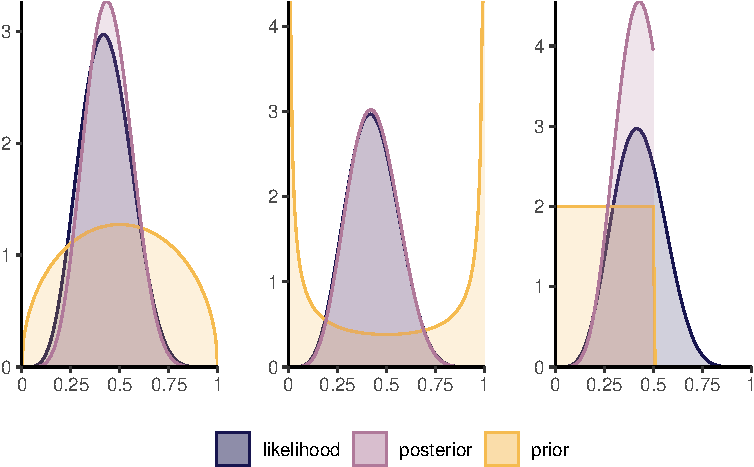
\includegraphics{introduction_files/figure-pdf/fig-betabinom-1.pdf}

}

\caption{\label{fig-betabinom}Scaled binomial likelihood for six
successes out of 14 trials, with \(\mathsf{Beta}(3/2, 3/2)\) prior
(left), \(\mathsf{Beta}(1/4, 1/4)\) (middle) and truncated uniform on
\([0,1/2]\) (right), with the corresponding posterior distributions.}

\end{figure}

\end{example}

\begin{remark}[Proportionality]

Any term appearing in the likelihood times prior function that does not
depend on parameters can be omitted since they will be absorbed by the
normalizing constant. This makes it useful to compute normalizing
constants or likelihood ratios.

\end{remark}

\begin{remark}

An alternative parametrization for the beta distribution sets
\(\alpha=\mu \kappa\), \(\beta = (1-\mu)\kappa\) for \(\mu \in (0,1)\)
and \(\kappa>0\), so that the model is parametrized directly in terms of
mean \(\mu\), with \(\kappa\) capturing the dispersion.

\end{remark}

\begin{remark}

A density integrates to 1 over the range of possible outcomes, but there
is no guarantee that the likelihood function, as a function of
\(\boldsymbol{\theta}\), integrates to one over the parameter domain
\(\boldsymbol{\Theta}\).

For example, the binomial likelihood with \(n\) trials and \(y\)
successes satisfies
\[\int_0^1 \binom{n}{y}\theta^y(1-\theta)^{n-y} \mathrm{d} \theta = \frac{1}{n+1}.\]

Moreover, the binomial distribution is discrete with support
\(0, \ldots, n\), whereas the likelihood is continuous as a function of
the probability of success, as evidenced by
Figure~\ref{fig-binom-massvslik}

\begin{figure}[ht!]

{\centering 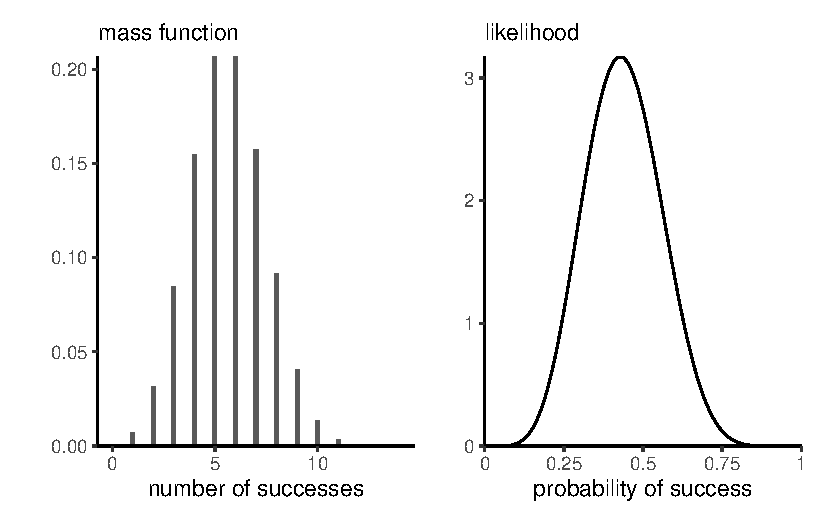
\includegraphics{introduction_files/figure-pdf/fig-binom-massvslik-1.pdf}

}

\caption{\label{fig-binom-massvslik}Binomial mass function (left) and
scaled likelihood function (right).}

\end{figure}

\end{remark}

\begin{proposition}[Sequentiality and Bayesian
updating]\protect\hypertarget{prp-sequentiality}{}\label{prp-sequentiality}

The likelihood is invariant to the order of the observations if they are
independent Thus, if we consider two blocks of observations
\(\boldsymbol{y}_1\) and \(\boldsymbol{y}_2\)
\[p(\boldsymbol{\theta} \mid \boldsymbol{y}_1, \boldsymbol{y}_2) = p(\boldsymbol{\theta} \mid \boldsymbol{y}_1) p(\boldsymbol{\theta} \mid \boldsymbol{y}_2),\]
so it makes no difference if we treat data all at once or in blocks.
More generally, for data exhibiting spatial or serial dependence, it
makes sense to consider rather the conditional (sequential)
decomposition
\[f(\boldsymbol{y}; \boldsymbol{\theta}) = f(\boldsymbol{y}_1; \boldsymbol{\theta}) f(\boldsymbol{y}_2; \boldsymbol{\theta}, \boldsymbol{y}_1) \cdots f(\boldsymbol{y}_n; \boldsymbol{\theta}, \boldsymbol{y}_1, \ldots, \boldsymbol{y}_{n-1})\]
where
\(f(\boldsymbol{y}_k; \boldsymbol{y}_1, \ldots, \boldsymbol{y}_{k-1})\)
denotes the conditional density function given observations
\(\boldsymbol{y}_1, \ldots, \boldsymbol{y}_{k-1}\).

By Bayes' rule, we can consider \emph{updating} the posterior by adding
terms to the likelihood, noting that \begin{align*}
p(\boldsymbol{\theta} \mid \boldsymbol{y}_1, \boldsymbol{y}_2) \propto p(\boldsymbol{y}_2 \mid \boldsymbol{y}_1, \boldsymbol{\theta}) p(\boldsymbol{\theta} \mid \boldsymbol{y}_1)
\end{align*} which amounts to treating the posterior
\(p(\boldsymbol{\theta} \mid \boldsymbol{y}_1)\) as a prior. If data are
exchangeable, the order in which observations are collected and the
order of the belief updating is irrelevant to the full posterior.
Figure~\ref{fig-sequential} shows how the posterior becomes gradually
closer to the scaled likelihood as we increase the sample size, and the
posterior mode moves towards the true value of the parameter (here 0.3).

\begin{figure}[ht!]

{\centering 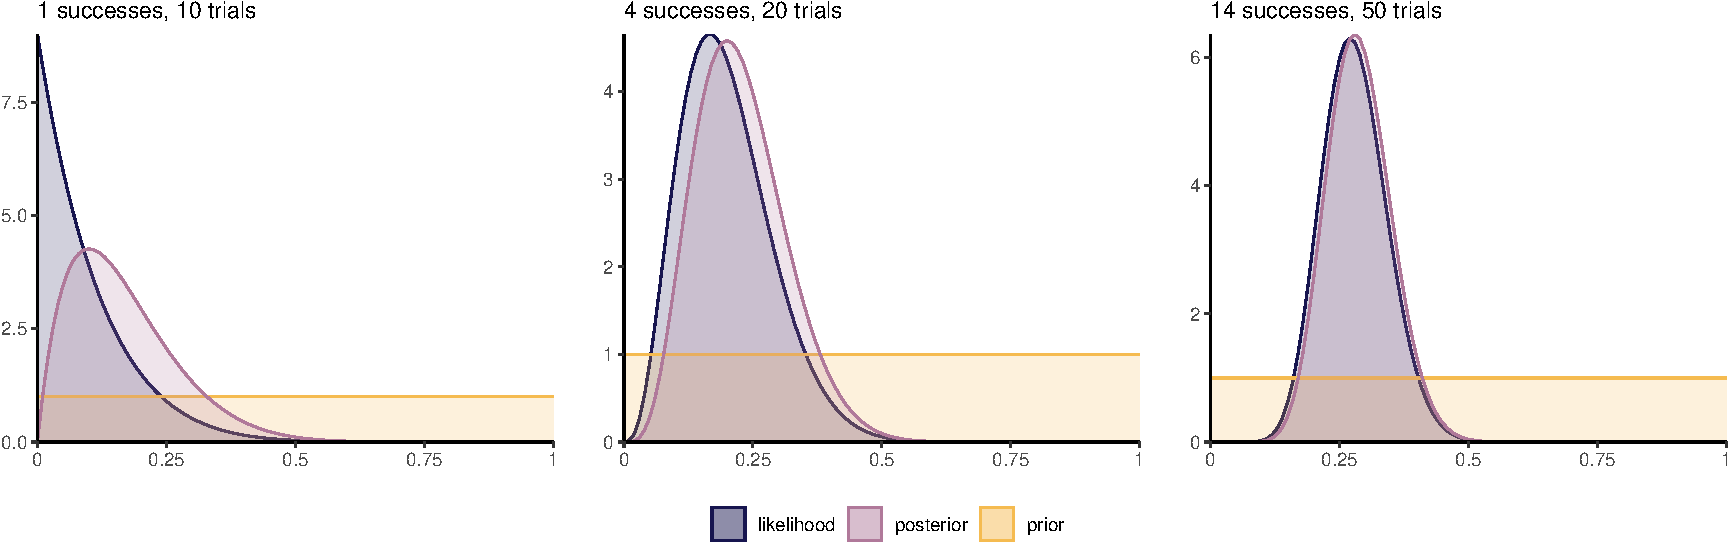
\includegraphics{introduction_files/figure-pdf/fig-sequential-1.pdf}

}

\caption{\label{fig-sequential}Beta posterior and binomial likelihood
with a uniform prior for increasing number of observations (from left to
right) out of a total of 100 trials.}

\end{figure}

\end{proposition}

\begin{example}[]\protect\hypertarget{exm-numericalintegration}{}\label{exm-numericalintegration}

While we can calculate analytically the value of the normalizing
constant for the beta-binomial model, we could also for arbitrary priors
use numerical integration or Monte Carlo methods in the event the
parameter vector \(\boldsymbol{\theta}\) is low-dimensional.

While estimation of the normalizing constant is possible in simple
models, the following highlights some challenges that are worth keeping
in mind. In a model for discrete data (that is, assigning probability
mass to a countable set of outcomes), the terms in the likelihood are
probabilities and thus the likelihood becomes smaller as we gather more
observations (since we multiply terms between zero or one). The marginal
likelihood term becomes smaller and smaller, so it's reciprocal is big
and this can lead to arithmetic underflow.

\begin{Shaded}
\begin{Highlighting}[]
\NormalTok{y }\OtherTok{\textless{}{-}}\NormalTok{ 6L }\CommentTok{\# number of successes }
\NormalTok{n }\OtherTok{\textless{}{-}}\NormalTok{ 14L }\CommentTok{\# number of trials}
\NormalTok{alpha }\OtherTok{\textless{}{-}}\NormalTok{ beta }\OtherTok{\textless{}{-}} \FloatTok{1.5} \CommentTok{\# prior parameters}
\NormalTok{unnormalized\_posterior }\OtherTok{\textless{}{-}} \ControlFlowTok{function}\NormalTok{(theta)\{}
\NormalTok{  theta}\SpecialCharTok{\^{}}\NormalTok{(y}\SpecialCharTok{+}\NormalTok{alpha}\DecValTok{{-}1}\NormalTok{) }\SpecialCharTok{*}\NormalTok{ (}\DecValTok{1}\SpecialCharTok{{-}}\NormalTok{theta)}\SpecialCharTok{\^{}}\NormalTok{(n}\SpecialCharTok{{-}}\NormalTok{y }\SpecialCharTok{+}\NormalTok{ beta }\SpecialCharTok{{-}} \DecValTok{1}\NormalTok{)}
\NormalTok{\}}
\FunctionTok{integrate}\NormalTok{(}\AttributeTok{f =}\NormalTok{ unnormalized\_posterior,}
          \AttributeTok{lower =} \DecValTok{0}\NormalTok{,}
          \AttributeTok{upper =} \DecValTok{1}\NormalTok{)}
\end{Highlighting}
\end{Shaded}

\begin{verbatim}
1.066906e-05 with absolute error < 1e-12
\end{verbatim}

\begin{Shaded}
\begin{Highlighting}[]
\CommentTok{\# Compare with known constant}
\FunctionTok{beta}\NormalTok{(y }\SpecialCharTok{+}\NormalTok{ alpha, n }\SpecialCharTok{{-}}\NormalTok{ y }\SpecialCharTok{+}\NormalTok{ beta)}
\end{Highlighting}
\end{Shaded}

\begin{verbatim}
[1] 1.066906e-05
\end{verbatim}

\begin{Shaded}
\begin{Highlighting}[]
\CommentTok{\# Monte Carlo integration}
\FunctionTok{mean}\NormalTok{(}\FunctionTok{unnormalized\_posterior}\NormalTok{(}\FunctionTok{runif}\NormalTok{(}\FloatTok{1e5}\NormalTok{)))}
\end{Highlighting}
\end{Shaded}

\begin{verbatim}
[1] 1.064067e-05
\end{verbatim}

\end{example}

When \(\boldsymbol{\theta}\) is high-dimensional, the marginal
likelihood is intractable. This is one of the main challenges of
Bayesian statistics and the popularity and applicability has grown
drastically with the development and popularity of numerical algorithms,
following the publication of Geman and Geman
(\protect\hyperlink{ref-Geman.Geman:1984}{1984}) and Gelfand and Smith
(\protect\hyperlink{ref-Gelfand.Smith:1990}{1990}). Markov chain Monte
Carlo methods circumvent the calculation of the denominator by drawing
approximate samples from the posterior.

\hypertarget{posterior-predictive-distribution}{%
\section{Posterior predictive
distribution}\label{posterior-predictive-distribution}}

Prediction in the Bayesian paradigm is obtained by considering the
\emph{posterior predictive distribution}, \begin{align*}
p(y_{\text{new}} \mid \boldsymbol{y}) =
\int_{\Theta} p(y_{\text{new}}  \mid \boldsymbol{\theta}) p(\boldsymbol{\theta} \mid  \boldsymbol{y}) \mathrm{d} \boldsymbol{\theta}
\end{align*}

Given draws from the posterior distribution, say
\(\boldsymbol{\theta}_b\) \((b=1, \ldots, B)\), we sample from each a
new realization from the distribution appearing in the likelihood
\(p(y_{\text{new}} \mid \boldsymbol{\theta}_b)\). This is different from
the frequentist setting, which fixes the value of the parameter to some
estimate \(\widehat{\boldsymbol{\theta}}\); by contrast, the posterior
predictive, here a beta-binomial distribution
\(\mathsf{BetaBin}(n, \alpha + y, n - y + \beta)\), carries over the
uncertainty so will typically be wider and overdispersed relative to the
corresponding binomial model. This can be easily seen from the
left-panel of Figure~\ref{fig-betabinompostpred}, which contrasts the
binomial mass function evaluated at the maximum likelihood estimator
\(\widehat{\theta}=6/14\) with the posterior predictive.

\begin{Shaded}
\begin{Highlighting}[]
\NormalTok{npost }\OtherTok{\textless{}{-}} \FloatTok{1e4}\NormalTok{L}
\CommentTok{\# Sample draws from the posterior distribution}
\NormalTok{post\_samp }\OtherTok{\textless{}{-}} \FunctionTok{rbeta}\NormalTok{(}\AttributeTok{n =}\NormalTok{ npost, y }\SpecialCharTok{+}\NormalTok{ alpha, n }\SpecialCharTok{{-}}\NormalTok{ y }\SpecialCharTok{+}\NormalTok{ beta)}
\CommentTok{\# For each draw, sample new observation}
\NormalTok{post\_pred }\OtherTok{\textless{}{-}} \FunctionTok{rbinom}\NormalTok{(}\AttributeTok{n =}\NormalTok{ npost, }\AttributeTok{size =}\NormalTok{ n, }\AttributeTok{prob =}\NormalTok{ post\_samp)}
\end{Highlighting}
\end{Shaded}

\begin{figure}[ht!]

{\centering 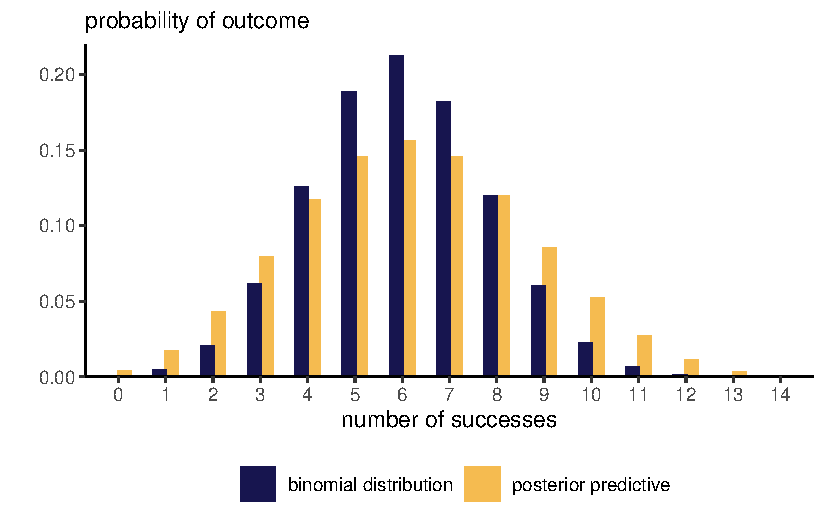
\includegraphics{introduction_files/figure-pdf/fig-betabinompostpred-1.pdf}

}

\caption{\label{fig-betabinompostpred}Beta-binomial posterior predictive
distribution with corresponding binomial mass function evaluated at the
maximum likelihood estimator.}

\end{figure}

\begin{example}[Posterior predictive distribution of univariate Gaussian
with known
mean]\protect\hypertarget{exm-normal-post-pred}{}\label{exm-normal-post-pred}

Consider an \(n\) sample of independent and identically distributed
Gaussian, \(Y_i \sim \mathsf{Norm}(0, \tau^{-1})\) (\(i=1, \ldots, n\)),
where we assign a gamma prior on the precision
\(\tau \sim \mathsf{Ga}(\alpha, \beta)\). The posterior is
\begin{align*}
p(\tau \mid \boldsymbol{y}) \stackrel{\tau}{\propto} \prod_{i=1}^n \tau^{n/2}\exp\left(-\tau \frac{\sum_{i=1}^n{y_i^2}}{2}\right) \times \tau^{\alpha-1} \exp(-\beta \tau)
\end{align*} and rearranging the terms to collect powers of \(\tau\),
etc. we find that the posterior for \(\tau\) must also be gamma, with
shape parameter \(\alpha^* = \alpha + n/2\) and rate
\(\beta^* = \beta + \sum_{i=1}^n y_i^2/2\).

The posterior predictive is \begin{align*}
p(y_{\text{new}} \mid \boldsymbol{y}) &= \int_0^\infty \frac{\tau^{1/2}}{(2\pi)^{1/2}}\exp(-\tau y_{\text{new}}^2/2) \frac{\beta^{*\alpha^*}}{\Gamma(\alpha^*)}\tau^{\alpha^*-1}\exp(-\beta^* \tau) \mathrm{d} \tau 
\\&= (2\pi)^{-1/2} \frac{\beta^{*\alpha^*}}{\Gamma(\alpha^*)} \int_0^\infty\tau^{\alpha^*-1/2} \exp\left\{- \tau (y_{\text{new}}^2/2 + \beta^*)\right\} \mathrm{d} \tau
\\&= (2\pi)^{-1/2} \frac{\beta^{*\alpha^*}}{\Gamma(\alpha^*)} \frac{\Gamma(\alpha^* + 1/2)}{(y_{\text{new}}^2/2 + \beta^*)^{\alpha^*+1/2}}
\\&= \frac{\Gamma\left(\frac{2\alpha^* + 1}{2}\right)}{\sqrt{2\pi}\Gamma\left(\frac{2\alpha^*}{2}\right)\beta^{*1/2}} \left( 1+ \frac{y_{\text{new}}^2}{2\beta^*}\right)^{-\alpha^*-1/2}
\\&= \frac{\Gamma\left(\frac{2\alpha^* + 1}{2}\right)}{\sqrt{\pi}\sqrt{ 2\alpha^*}\Gamma\left(\frac{2\alpha^*}{2}\right)(\beta^*/\alpha^*)^{1/2}} \left( 1+ \frac{1}{2\alpha^*}\frac{y_{\text{new}}^2}{(\beta^*/\alpha^*)}\right)^{-\alpha^*-1/2}
\end{align*} which entails that \(Y_{\text{new}}\) is a scaled
Student-\(t\) distribution with scale \((\beta^*/\alpha^*)^{1/2}\) and
\(2\alpha+n\) degrees of freedom. This example also exemplifies the
additional variability relative to the distribution generating the data:
indeed, the Student-\(t\) distribution is more heavy-tailed than the
Gaussian, but since the degrees of freedom increase linearly with \(n\),
the distribution converges to a Gaussian as \(n \to \infty\), reflecting
the added information as we collect more and more data points and the
variance gets better estimated through \(\sum_{i=1}^n y_i^2/n\).

\end{example}

\hypertarget{summarizing-posterior-distributions}{%
\section{Summarizing posterior
distributions}\label{summarizing-posterior-distributions}}

The output of the Bayesian learning problem will be either of:

\begin{enumerate}
\def\labelenumi{\arabic{enumi}.}
\tightlist
\item
  a fully characterized distribution
\item
  a numerical approximation to the posterior distribution (pointwise)
\item
  an exact or approximate sample drawn from the posterior distribution
\end{enumerate}

In the first case, we will be able to directly evaluate quantities of
interest if there are closed-form expressions for the latter, or else we
could draw samples from the distribution and evaluate them via
Monte-Carlo. In case of numerical approximations, we will need to resort
to numerical integration or otherwise to get our answers.

Often, we will also be interested in the marginal posterior distribution
of each component \(\theta_j\) in turn (\(j=1, \ldots, J\)). To get
these, we carry out additional integration steps,
\[p(\theta_j \mid \boldsymbol{y}) = \int p(\boldsymbol{\theta} \mid \boldsymbol{y}) \mathrm{d} \boldsymbol{\theta}_{-j}.\]
With a posterior sample, this is trivial: it suffices to keep the column
corresponding to \(\theta_j\) and discard the others.

Most of the field of Bayesian statistics revolves around the creation of
algorithms that either circumvent the calculation of the normalizing
constant (notably using Monte Carlo and Markov chain Monte Carlo
methods) or else provide accurate numerical approximation of the
posterior pointwise, including for marginalizing out all but one
parameters (integrated nested Laplace approximations, variational
inference, etc.) The target of inference is the whole posterior
distribution, a potentially high-dimensional object which may be
difficult to summarize or visualize. We can thus report only
characteristics of the the latter.

The choice of point summary to keep has it's root in decision theory.

\begin{definition}[Loss
function]\protect\hypertarget{def-lossfunction}{}\label{def-lossfunction}

A loss function \(c(\boldsymbol{\theta}, \boldsymbol{\upsilon})\) is a
mapping from \(\boldsymbol{\Theta} \to \mathbb{R}^k\) that assigns a
weight to each value of \(\boldsymbol{\theta}\), corresponding to the
regret or loss arising from choosing this value. The corresponding point
estimator \(\widehat{\boldsymbol{\upsilon}}\) is the minimizer of the
expected loss,

\begin{align*}
\widehat{\boldsymbol{\upsilon}} &= \mathop{\mathrm{argmin}}_{\boldsymbol{\upsilon}}\mathsf{E}_{\boldsymbol{\Theta} \mid \boldsymbol{Y}}\{c(\boldsymbol{\theta}, \boldsymbol{v})\} \\&=\mathop{\mathrm{argmin}}_{\boldsymbol{\upsilon}} \int_{\boldsymbol{\Theta}} c(\boldsymbol{\theta}, \boldsymbol{\upsilon})p(\boldsymbol{\theta} \mid \boldsymbol{y}) \mathrm{d} \boldsymbol{\theta}
\end{align*}

\end{definition}

For example, in a univariate setting, the quadratic loss
\(c(\theta, \upsilon) = (\theta-\upsilon)^2\) returns the posterior
mean, the absolute loss \(c(\theta, \upsilon)=|\theta - \upsilon|\)
returns the posterior median and the 0-1 loss
\(c(\theta, \upsilon) = \mathrm{I}(\upsilon \neq \theta)\) returns the
posterior mode. All of these point estimators are central tendency
measures, but some may be more adequate depending on the setting as they
can correspond to potentially different values, as shown in the
left-panel of Figure~\ref{fig-central-moments}. The choice is
application specific: for multimodal distributions, the mode is likely a
better choice.

If we know how to evaluate the distribution numerically, we can optimize
to find the mode or else return the value for the pointwise evaluation
on a grid at which the density achieves it's maximum. The mean and
median would have to be evaluated by numerical integration if there is
no closed-form expression for the latter.

If we have rather a sample from the posterior with associated posterior
density values, then we can obtain the mode as the parameter combination
with the highest posterior, the median from the value at rank
\(\lfloor n/2\rfloor\) and the mean through the sample mean of posterior
draws.

\begin{figure}[ht!]

{\centering 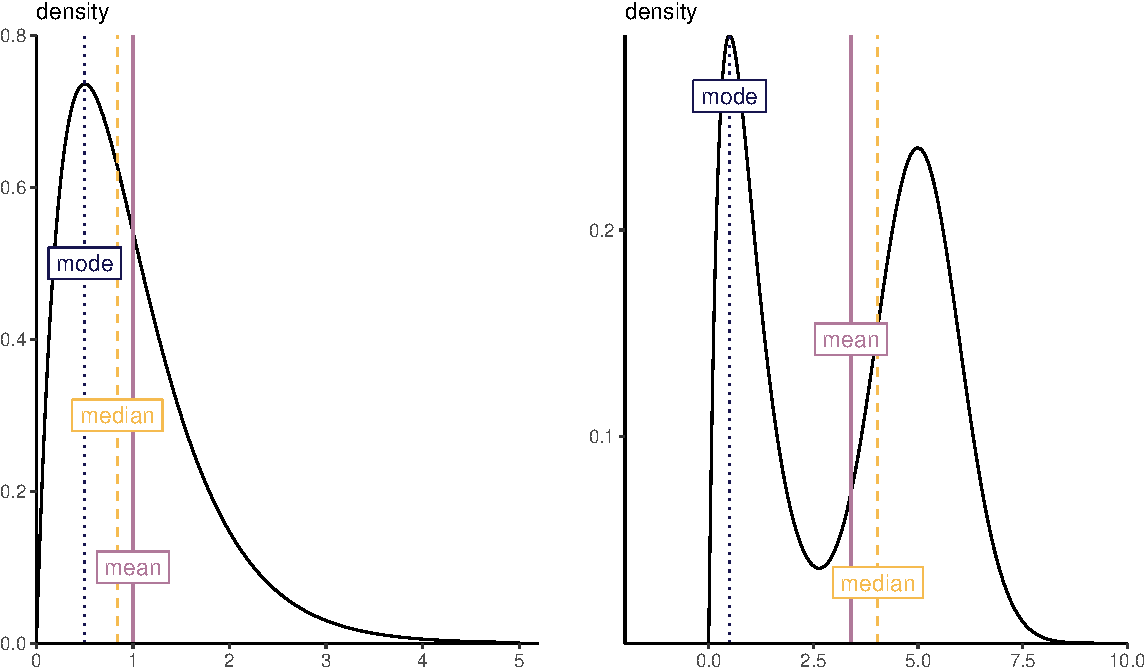
\includegraphics{introduction_files/figure-pdf/fig-central-moments-1.pdf}

}

\caption{\label{fig-central-moments}Point estimators from a right-skewed
distribution (left) and from a multimodal distribution (right).}

\end{figure}

The loss function is often a functional (meaning a one-dimensional
summary) from the posterior. The following example shows how it reduces
a three-dimensional problem into a single risk measure.

\begin{example}[Danish insurance
losses]\protect\hypertarget{exm-loss-extremes}{}\label{exm-loss-extremes}

In extreme value, we are often interested in assessing the risk of
events that are rare enough that they lie beyond the range of observed
data. To provide a scientific extrapolation, it often is justified to
fit a generalized Pareto distribution to exceedances of \(Z=Y-u\), for
some user-specified threshold \(u\) which is often taken as a large
quantile of the distribution of \(Y\). The generalized Pareto
distribution function is \begin{align*}
F(z; \tau, \xi) = 1- \begin{cases}
\left(1+\xi/\tau z\right)^{-1/\xi}_{+}, & \xi \neq 0\\
\exp(-z/\tau), & \xi = 0. \end{cases}
\end{align*} The shape \(\xi\) governs how heavy-tailed the distribution
is, while \(\tau\) is a scale parameter.

Insurance companies provide coverage in exchange for premiums, but need
to safeguard themselves against very high claims by buying reinsurance
products. These risks are often communicated through the value-at-risk
(VaR), a high quantile exceeded with probability \(p\). We model Danish
fire insurance claim amounts for inflation-adjusted data collected from
January 1980 until December 1990 that are in excess of a million Danish
kroner, found in the \texttt{evir} package and analyzed in Example 7.23
of McNeil, Frey, and Embrechts
(\protect\hyperlink{ref-McNeil.Frey.Embrechts:2005}{2005}). These claims
are denoted \(Y\) and there are 2167 observations.

We fit a generalized Pareto distribution to exceedances above 10
millions krones, keeping 109 observations or roughly the largest 5\% of
the original sample. Preliminary analysis shows that we can treat data
as roughly independent and identically distributed and goodness-of-fit
diagnostics (not shown) for the generalized Pareto suggest that the fit
is adequate for all but the three largest observations, which are
(somewhat severely) underestimated by the model.

\begin{figure}[ht!]

{\centering 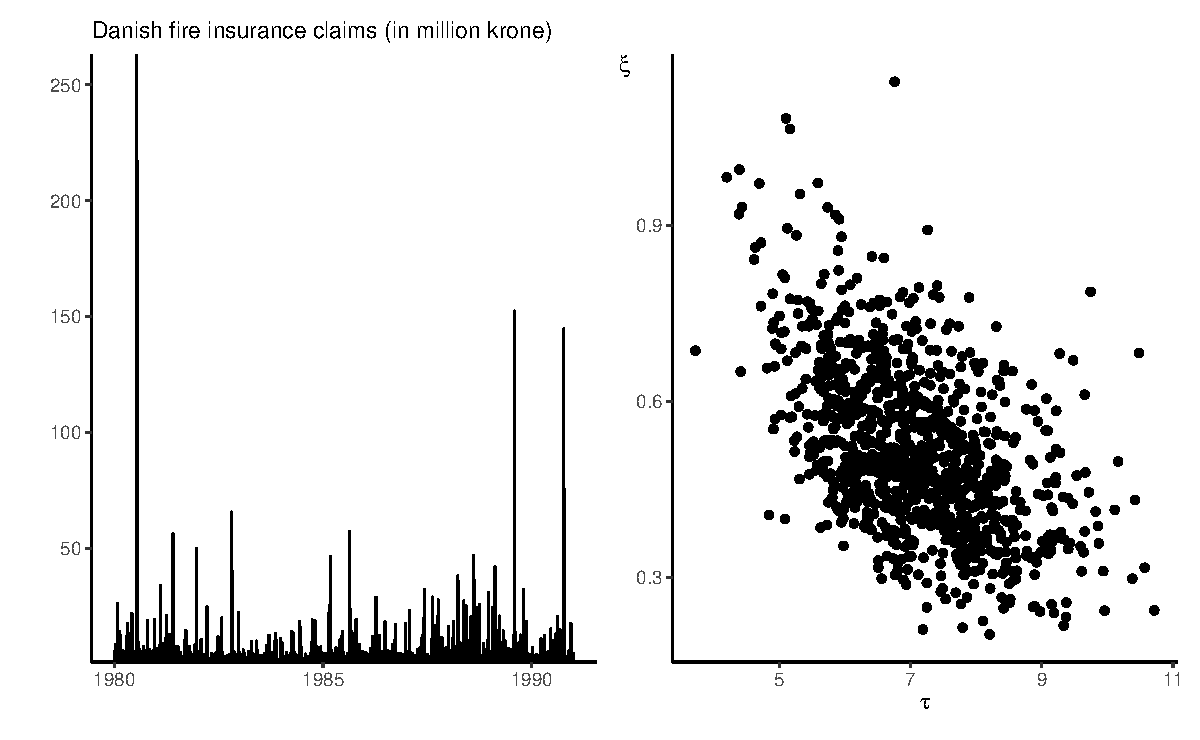
\includegraphics{introduction_files/figure-pdf/fig-danish-1.pdf}

}

\caption{\label{fig-danish}Time series of Danish fire claims exceeding a
million krone (left) and posterior samples from the scale \(\tau\) and
shape \(\xi\) of the generalized Pareto model fitted to exceedances
above 10 million krone (right).}

\end{figure}

The generalized Pareto model only describes the \(n_u\) exceedances
above \(u=10\), so we need to incorporate in the likelihood a binomial
contribution for the probability \(\zeta_u\) of exceeding the threshold
\(u\). Provided that the priors for \((\tau, \xi)\) are independent of
those for \(\zeta_u\), the posterior also factorizes as a product, so
\(\zeta_u\) and \((\tau, \xi)\) are a posteriori independent.

Suppose for now that we set a \(\mathsf{Beta}(0.5, 0.5)\) prior for
\(\zeta_u\) and a non-informative prior for the generalized Pareto
parameters. The \texttt{post\_samp} matrix contains exact samples from
the posterior distribution of \((\tau, \xi, \zeta_u)\), obtained using a
Monte Carlo algorithm. Our aim is to evaluate the posterior distribution
for the value-at-risk, the \(\alpha\) quantile of \(Y\) for high values
of \(\alpha\) and see what point estimator one would obtain depending on
our choice of loss function. For any \(\alpha > 1-\zeta_u\), the
\(q_{\alpha}\) is \begin{align*}
1- \alpha  &= \Pr(Y > q_\alpha \mid Y > u) \Pr(Y > u) 
\\ &= \left(1+\xi \frac{q_{\alpha}-u}{\tau}\right)_{+}^{-1/\xi}\zeta_u
\end{align*} and solving for \(q_{\alpha}\) gives \begin{align*}
q_{\alpha} = u+ \frac{\tau}{\xi} \left\{\left(\frac{\zeta_u}{1-\alpha}\right)^\xi-1\right\}.
\end{align*}

To obtain the posterior distribution of the \(\alpha\) quantile,
\(q_{\alpha}\), it suffices to plug in each posterior sample and
evaluate the function: the uncertainty is carried over from the
simulated values of the parameters to those of the quantile
\(q_{\alpha}\). The left panel of Figure~\ref{fig-lossfn} shows the
posterior density estimate of the \(\mathsf{VaR}(0.99)\) along with the
maximum a posteriori (mode) of the latter.

Suppose that we prefer to under-estimate the value-at-risk rather than
overestimate: this could be captured by the custom loss function
\begin{align*}
c(q, q_0) = 
\begin{cases}
0.5(0.99q - q_0), & q > q_0 \\
0.75(q_0 - 1.01q), & q < q_0.
\end{cases}
\end{align*} For a given value of the value-at-risk \(q_0\) evaluated on
a grid, we thus compute \begin{align*}
 r(q_0) = \int_{\boldsymbol{\Theta}}c(q(\boldsymbol{\theta}), q_0) p (\boldsymbol{\theta} \mid \boldsymbol{y}) \mathrm{d} \boldsymbol{\theta}
\end{align*} and we seek to minimize the risk,
\(\widehat{q} =\mathrm{argmin}_{q_0 \in \mathbb{R}_{+}} r(q_0)\). The
value returned that minimizes the loss, shown in
Figure~\ref{fig-lossfn}, is to the left of the posterior mean for
\(q_\alpha\).

\begin{Shaded}
\begin{Highlighting}[]
\CommentTok{\# Compute value at risk from generalized Pareto distribution quantile fn}
\NormalTok{VaR\_post }\OtherTok{\textless{}{-}} \FunctionTok{with}\NormalTok{(post\_samp,   }\CommentTok{\# data frame of posterior draws}
\NormalTok{            revdbayes}\SpecialCharTok{::}\FunctionTok{qgp}\NormalTok{(   }\CommentTok{\# with columns \textquotesingle{}probexc\textquotesingle{}, \textquotesingle{}scale\textquotesingle{}, \textquotesingle{}shape\textquotesingle{}}
  \AttributeTok{p =} \FloatTok{0.01}\SpecialCharTok{/}\NormalTok{probexc, }
  \AttributeTok{loc =} \DecValTok{10}\NormalTok{, }
  \AttributeTok{scale =}\NormalTok{ scale, }
  \AttributeTok{shape =}\NormalTok{ shape, }
  \AttributeTok{lower.tail =} \ConstantTok{FALSE}\NormalTok{))}
\CommentTok{\# Loss function}
\NormalTok{loss }\OtherTok{\textless{}{-}} \ControlFlowTok{function}\NormalTok{(qhat, q)\{}
    \FunctionTok{mean}\NormalTok{(}\FunctionTok{ifelse}\NormalTok{(q }\SpecialCharTok{\textgreater{}}\NormalTok{ qhat,}
           \FloatTok{0.5}\SpecialCharTok{*}\NormalTok{(}\FloatTok{0.99}\SpecialCharTok{*}\NormalTok{q}\SpecialCharTok{{-}}\NormalTok{qhat),}
           \FloatTok{0.75}\SpecialCharTok{*}\NormalTok{(qhat}\FloatTok{{-}1.01}\SpecialCharTok{*}\NormalTok{q)))}
\NormalTok{\}}
\CommentTok{\# Create a grid of values over which to estimate the loss for VaR}
\NormalTok{nvals }\OtherTok{\textless{}{-}}\NormalTok{ 101L}
\NormalTok{VaR\_grid }\OtherTok{\textless{}{-}} \FunctionTok{seq}\NormalTok{(}
  \AttributeTok{from =} \FunctionTok{quantile}\NormalTok{(VaR\_post, }\FloatTok{0.01}\NormalTok{),}
  \AttributeTok{to =} \FunctionTok{quantile}\NormalTok{(VaR\_post, }\FloatTok{0.99}\NormalTok{), }
  \AttributeTok{length.out =}\NormalTok{ nvals)}
\CommentTok{\# Create a container to store results}
\NormalTok{risk }\OtherTok{\textless{}{-}} \FunctionTok{numeric}\NormalTok{(}\AttributeTok{length =}\NormalTok{ nvals)}
\ControlFlowTok{for}\NormalTok{(i }\ControlFlowTok{in} \FunctionTok{seq\_len}\NormalTok{(nvals))\{}
  \CommentTok{\# Compute integral (Monte Carlo average over draws)}
\NormalTok{ risk[i] }\OtherTok{\textless{}{-}} \FunctionTok{loss}\NormalTok{(}\AttributeTok{q =}\NormalTok{ VaR\_post, }\AttributeTok{qhat =}\NormalTok{ VaR\_grid[i])}
\NormalTok{\}}
\end{Highlighting}
\end{Shaded}

\begin{figure}[ht!]

{\centering 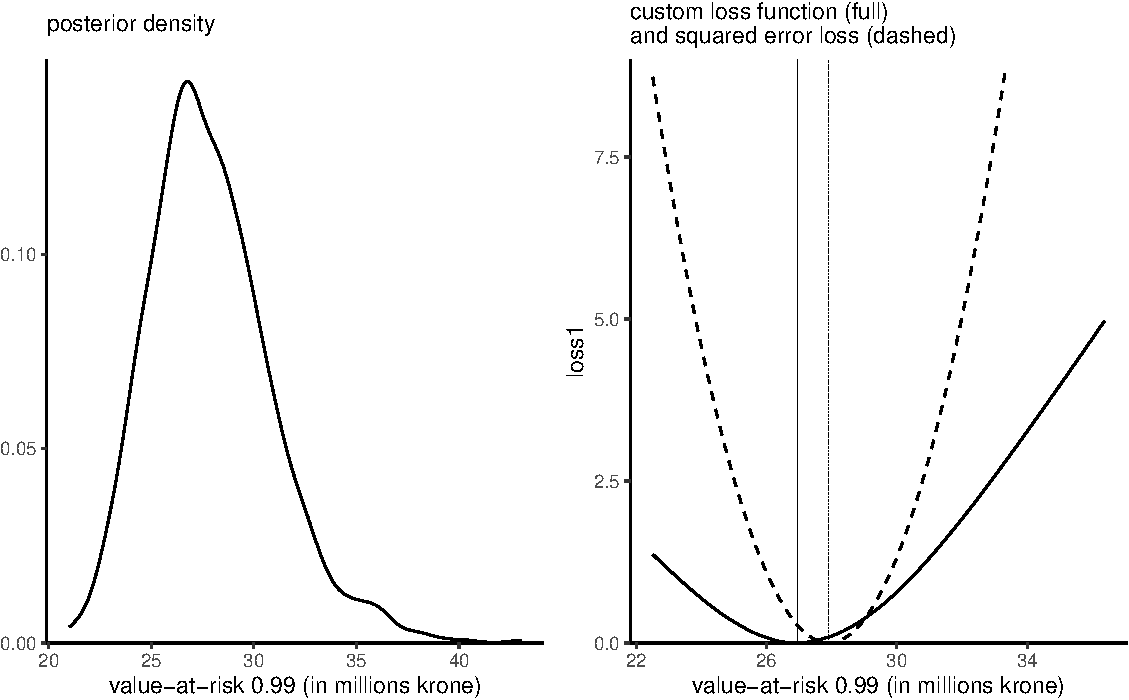
\includegraphics{introduction_files/figure-pdf/fig-lossfn-1.pdf}

}

\caption{\label{fig-lossfn}Posterior density (left) and losses functions
for the 0.99 value-at-risk for the Danish fire insurance data. The
vertical lines denote point estimates of the quantiles that minimize the
loss functions.}

\end{figure}

\end{example}

To communicate uncertainty, we may resort to credible regions and
intervals.

\begin{definition}[]\protect\hypertarget{def-credible-region}{}\label{def-credible-region}

A \((1-\alpha)\) \textbf{credible region} (or credible interval in the
univariate setting) is a set \(\mathcal{S}_\alpha\) such that, with
probability level \(\alpha\), \begin{align*}
\Pr(\boldsymbol{\theta} \in \mathcal{S}_\alpha \mid \boldsymbol{Y}=\boldsymbol{y}) = 1-\alpha
\end{align*}

\end{definition}

These intervals are not unique, as are confidence sets. In the
univariate setting, the central or equitailed interval are the most
popular, and easily obtained by considering the \(\alpha/2, 1-\alpha/2\)
quantiles. These are easily obtained from samples by simply taking
empirical quantiles. An alternative, highest posterior density credible
sets, which may be a set of disjoint intervals obtained by considering
the parts of the posterior with the highest density, may be more
informative. The top panel Figure~\ref{fig-credible-intervals} shows the
distinction for a bimodal mixture distribution, and a even more striking
difference for 50\% credible intervals for a symmetric beta distribution
whose mass lie near the endpoints of the distribution, leading to no
overlap between the two intervals.

\begin{figure}[ht!]

{\centering 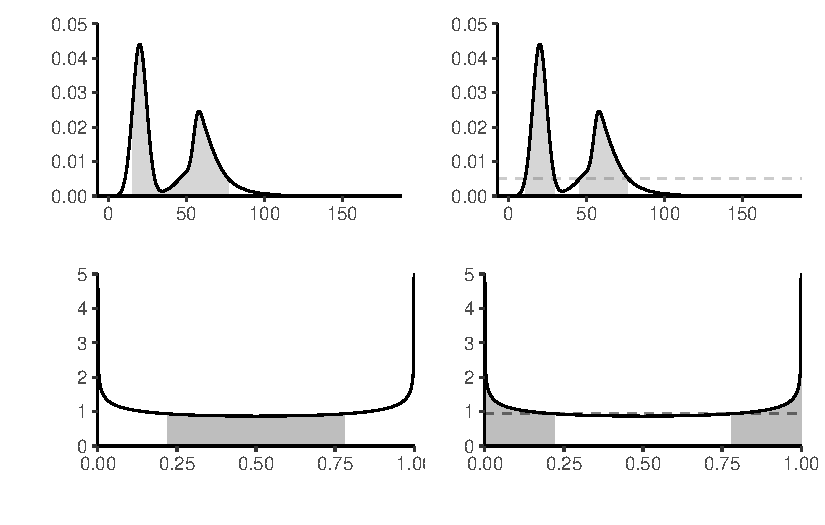
\includegraphics{introduction_files/figure-pdf/fig-credible-intervals-1.pdf}

}

\caption{\label{fig-credible-intervals}Density plots with 89\% (top) and
50\% (bottom) equitailed or central credible (left) and highest
posterior density (right) regions for two data sets, highlighted in
grey. The horizontal lign gives the posterior density value determining
the cutoff for the HDP region.}

\end{figure}

\begin{verbatim}



`<!-- quarto-file-metadata: eyJyZXNvdXJjZURpciI6Ii4ifQ== -->`{=html}

```{=html}
<!-- quarto-file-metadata: eyJyZXNvdXJjZURpciI6Ii4iLCJib29rSXRlbVR5cGUiOiJjaGFwdGVyIiwiYm9va0l0ZW1OdW1iZXIiOjIsImJvb2tJdGVtRmlsZSI6InByaW9ycy5xbWQiLCJib29rSXRlbURlcHRoIjowfQ== -->
\end{verbatim}

\bookmarksetup{startatroot}

\hypertarget{priors}{%
\chapter{Priors}\label{priors}}

The posterior distribution combines two ingredients: the likelihood and
the prior. If the former is a standard ingredient of any
likelihood-based inference, prior specification requires some care. The
purpose of this chapter is to consider different standard way of
constructing prior functions, and to specify the parameters of the
latter: we term these hyperparameters.

The posterior is a compromise prior and likelihood: the more informative
the prior, the more the posterior resembles it, but in large samples,
the effect of the prior is often negligible if there is enough
information in the likelihood about all parameters. We can assess the
robustness of the prior specification through a sensitivity analysis by
comparing the outcomes of the posterior for different priors or
different values of the hyperparameters.

We can use moment matching to get sensible values, or tune via
trial-and-error using the prior predictive draws to assess the
implausibility of the prior outcomes. One challenge is that even if we
have some prior information (e.g., we can obtain sensible prior values
for the mean, quantiles or variance of the parameter of interest), these
summary statisticss will not typically be enough to fully characterize
the prior: many different functions or distributions could encode the
same information. This means that different analysts get different
inferences. Generally, we will choose the prior for convenience. Priors
are controversial because they could be tuned aposteriori to give any
answer an analyst might want.

\hypertarget{prior-simulation}{%
\section{Prior simulation}\label{prior-simulation}}

Expert elicitation is difficult and it is hard to grasp what the impacts
of the hyperparameters are. One way to see if the priors are reasonable
is to sample values from them and generate new observations, resulting
in prior predictive draws.

The prior predictive is
\(\int_{\boldsymbol{\Theta}} p(y \mid \boldsymbol{\theta}) p(\boldsymbol{\theta}) \mathrm{d} \boldsymbol{\theta}\):
we can simulate outcomes from it by first drawing parameter values from
the prior, then sampling new observations from the distribution in the
likelihood and keeping only the latter. If there are sensible bounds for
the range of the response, we could discard values that do not abide
with these.

Working with standardized inputs
\(x_i \mapsto (x_i - \overline{x})/\mathrm{sd}(\boldsymbol{x})\) is
useful. For example, in a simple linear regression (with a sole
numerical explanatory), the slope is the correlation between
standardized explanatory \(\mathrm{X}\) and standardized response \(Y\)
and the intercept should be mean zero.

\begin{example}[]\protect\hypertarget{exm-bixi-temp}{}\label{exm-bixi-temp}

Consider the daily number of Bixi bike sharing users for 2017--2019 at
the Edouard Montpetit station next to HEC: we can consider a simple
linear regression with log counts as a function of
temperature,\footnote{If counts are Poisson, then the log transform is
  variance stabilizing.}
\[\log (\texttt{nusers}) \sim \mathsf{Norm}_{+}\{\beta_0 + \beta_1 (\texttt{temp}-20), \sigma^2\}.\]
The \(\beta_1\) slope measures units in degree Celsius per log number of
person.

The hyperparameters depend of course on the units of the analysis,
unless one standardizes response variable and explanatories: it is
easier to standardize the temperature so that we consider deviations
from, say 20\(^{\circ}\)C, which is not far from the observed mean in
the sample. After some tuning, the independent priors
\(\beta_0 \sim \mathsf{Norm}(\overline{y}, 0.5^2)\),
\(\beta_1 \sim \mathsf{Norm}(0, 0.05^2)\) and
\(\sigma \sim \mathsf{Exp}(3)\) seem to yield plausible outcomes and
relationships.\footnote{One can object to the prior parameters depending
  on the data, but an alternative would be to model centered data
  \(y-\overline{y}\), in which case the prior for the intercept
  parameter \(\beta_0\) would be zero.}

\begin{figure}[ht!]

{\centering 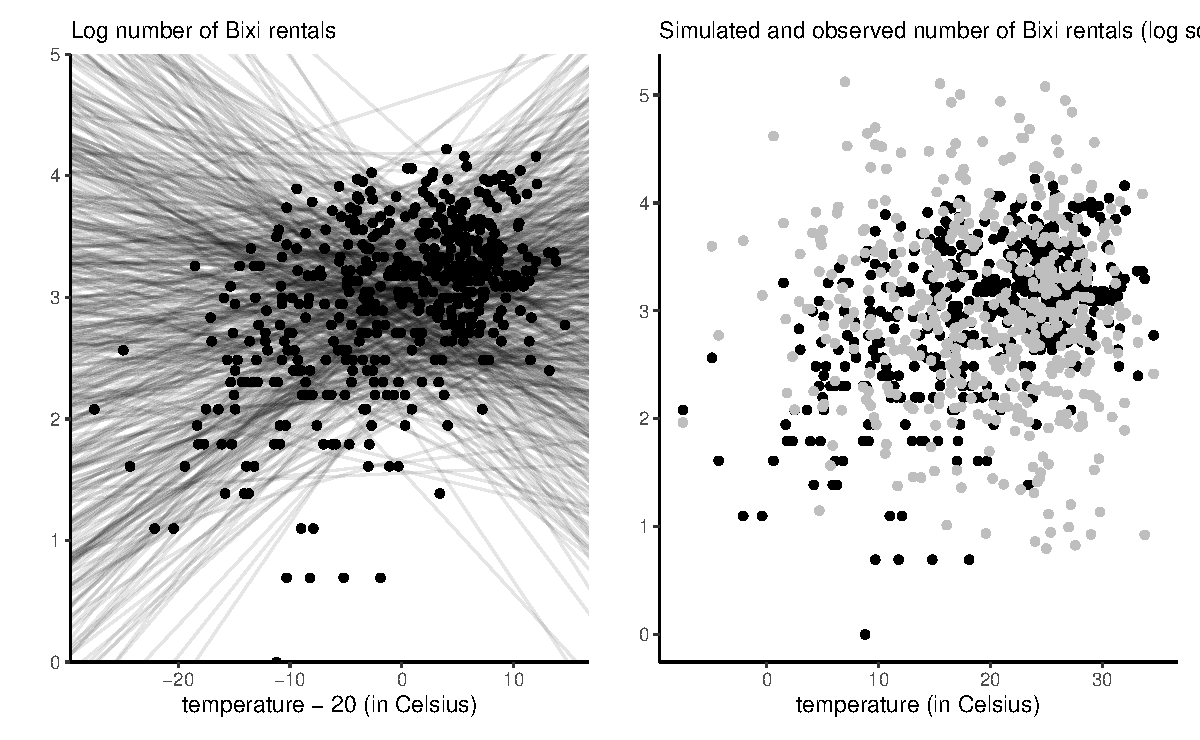
\includegraphics{priors_files/figure-pdf/fig-bixi-1.pdf}

}

\caption{\label{fig-bixi}Prior draws of the linear regressions with
observed data superimposed (left), and draws of observations from the
prior predictive distribution (in gray) against observed data (right).}

\end{figure}

We can draw regression lines from the prior, as in the left panel of
Figure~\ref{fig-bixi}: while some of the negative relationships appear
unlikely after seeing the data, the curves all seem to pass somewhere in
the cloud of point. By contrast, a silly prior is one that would result
in all observations being above or below the regression line, or yield
values that are much too large near the endpoints of the explanatory
variable. Indeed, given the number of bikes for rental is limited (a
docking station has only 20 bikes), it is also sensible to ensure that
simulations do not return overly large numbers. The maximum number of
daily users in the sample is 68, so priors that return simulations with
more than 200 (rougly 5.3 on the log scale) are not that plausible. The
prior predictive draws can help establish this and the right panel of
Figure~\ref{fig-bixi} shows that, expect for the lack of correlation
between temperature and number of users, the simulated values from the
prior predictive are plausible even if overdispersed.

\end{example}

\hypertarget{conjugate-priors}{%
\section{Conjugate priors}\label{conjugate-priors}}

In very simple models, there may exists prior densities that result in a
posterior distribution of the same family. We can thus directly extract
characteristics of the posterior. Conjugate priors are chosen for
computational convenience and because interpretation is convenient, as
the parameters of the posterior will often be some weighted average of
prior and likelihood component.

\begin{definition}[]\protect\hypertarget{def-conjugate-prior}{}\label{def-conjugate-prior}

A prior density \(p(\boldsymbol{\theta})\) is conjugate for likelihood
\(L(\boldsymbol{\theta}; \boldsymbol{y})\) if the product
\(L(\boldsymbol{\theta}; \boldsymbol{y})p(\boldsymbol{\theta})\), after
renormalization, is of the same parametric family as the prior.

Exponential families (including the binomial, Poisson, exponential,
Gaussian distributions) admit conjugate priors\footnote{A distribution
  belongs to an exponential family with parameter vector
  \(\boldsymbol{\theta} \in \mathbb{R}^D\) if it can be written as
  \begin{align*}
  f(y; \boldsymbol{\theta}) = \exp\left\{ \sum_{k=1}^K Q_k(\boldsymbol{\theta}) t_k(y) + D(\boldsymbol{\theta})\right\}
  \end{align*} and in particular, the support does not depend on unknown
  parameters. If we have an independent and identically distributed
  sample of observations \(y_1, \ldots, y_n\), the log likelihood is
  thus of the form \begin{align*}
  \ell(\boldsymbol{\theta}) = \sum_{k=1}^K \phi_k(\boldsymbol{\theta}) \sum_{i=1}^n t_k(y_i) + n D(\boldsymbol{\theta}),
  \end{align*} where the collection \(\sum_{i=1}^n t_k(y_i)\)
  (\(k=1, \ldots, K\)) are sufficient statistics and
  \(\phi_k(\boldsymbol{\theta})\) are the canonical parameters. The
  number of sufficient statistics are the same regardless of the sample
  size. Exponential families play a prominent role in generalized linear
  models, in which the natural parameters are modeled as linear function
  of explanatory variables. A log prior density with parameters
  \(\eta, \nu_1, \ldots, \nu_K\) that is proportional to \begin{align*}
  \log p(\boldsymbol{\theta}) \propto \eta D(\boldsymbol{\theta}) + \sum_{k=1}^K Q_k(\boldsymbol{\theta}) \nu_k
  \end{align*} is conjugate.}

\end{definition}

\begin{example}[Conjugate prior for the binomial
model]\protect\hypertarget{exm-conjugatepriors-binom}{}\label{exm-conjugatepriors-binom}

The binomial log density with \(y\) successes out of \(n\) trials is
proportional to \begin{align*}
y \log(p) + (n-y) \log(1-p) = y\log\left( \frac{p}{1-p}\right) + n \log(1-p)
\end{align*} with canonical parameter \(\mathrm{logit}(p)\).\footnote{The
  canonical link function for Bernoulli gives rise to logistic
  regression model.} The binomial distribution is thus an exponential
family.

Since the density of the binomial is of the form \(p^y(1-p)^{n-y}\), the
beta distribution \(\mathsf{Beta}(\alpha, \beta)\) with density
\[f(x) \propto x^{\alpha-1} (1-x)^{\beta-1}\] is the conjugate prior.

The beta distribution is also the conjugate prior for the negative
binomial, geometric and Bernoulli distributions, since their likelihoods
are all proportional to that of the beta. The fact that different
sampling schemes that result in proportional likelihood functions give
the same inference is called likelihood principle.

\end{example}

\begin{example}[Conjugate prior for the Poisson
model]\protect\hypertarget{exm-conjugatepriors-poisson}{}\label{exm-conjugatepriors-poisson}

The Poisson distribution with mean \(\mu\) has log density proportional
to \(f(y; \mu) \propto y\log(\mu) -\mu\), so is an exponential family
with natural parameter \(\log(\mu)\). The gamma density,
\[ f(x) \propto \beta^{\alpha}/\Gamma(\alpha)x^{\alpha-1} \exp(-\beta x)\]
with shape \(\alpha\) and rate \(\beta\) is the conjugate prior for the
Poisson. For an \(n\)-sample of independent observations
\(\mathsf{Pois}(\mu)\) observations with
\(\mu \sim \mathsf{Gamma}(\alpha, \beta)\), the posterior is
\(\mathsf{Gamma}(\sum_{i=1}^n y_i + \alpha, \beta + n)\).

\end{example}

Knowing the analytic expression for the posterior can be useful for
calculations of the marginal likelihood, as
Example~\ref{exm-poisson-negbin} demonstrates.

\begin{example}[Negative binomial as a Poisson
mixture]\protect\hypertarget{exm-poisson-negbin}{}\label{exm-poisson-negbin}

~

One restriction of the Poisson model is that the restriction on its
moments is often unrealistic. The most frequent problem encountered is
that of \textbf{overdispersion}, meaning that the variability in the
counts is larger than that implied by a Poisson distribution.

One common framework for handling overdispersion is to have
\(Y \mid \Lambda = \lambda \sim \mathsf{Pois}(\lambda)\), where the mean
of the Poisson distribution is itself a positive random variable with
mean \(\mu\), if \(\Lambda\) follows a conjugate gamma distribution with
shape \(k\mu\) and rate \(k>0\),
\(\Lambda \sim \mathsf{Gamma}(k\mu, k)\), the posterior
\(\Lambda \mid Y=y \sim \mathsf{Gamma}(k\mu + y, k+1)\).

Since the joint density of \(Y\) and \(\Lambda\) can be written \[
p(y, \lambda) = p(y \mid \lambda)p(\lambda) = p(\lambda \mid y) p(y)
\] we can isolate the marginal density \begin{align*}
p(y) &= \frac{p(y \mid \lambda)p(\lambda)}{p(\lambda \mid y)} \\&= \frac{\frac{\lambda^y\exp(-\lambda)}{\Gamma(y+1)}  \frac{k^{k\mu}\lambda^{k\mu-1}\exp(-k\lambda)}{\Gamma(k\mu)}}{ \frac{(k+1)^{k\mu+y}\lambda^{k\mu+y-1}\exp\{-(k+1)\lambda\}}{\Gamma(k\mu+y)}}\\
&= \frac{\Gamma(k\mu+y)}{\Gamma(k\mu)\Gamma(y+1)}k^{k\mu} (k+1)^{-k\mu-y}\\&= \frac{\Gamma(k\mu+y)}{\Gamma(k\mu)\Gamma(y+1)}\left(1-\frac{1}{k+1}\right)^{k\mu} \left(\frac{1}{k+1}\right)^y
\end{align*} and this is the density of a negative binomial distribution
with probability of success \(1/(k+1)\). We can thus view the negative
binomial as a Poisson mean mixture.

By the laws of iterated expectation and iterative variance,
\begin{align*}
\mathsf{E}(Y) &= \mathsf{E}_{\Lambda}\{\mathsf{E}(Y \mid \Lambda\} \\& = \mathsf{E}(\Lambda) = \mu\\
\mathsf{Va}(Y) &= \mathsf{E}_{\Lambda}\{\mathsf{Va}(Y \mid \Lambda)\} + \mathsf{Va}_{\Lambda}\{\mathsf{E}(Y \mid \Lambda)\} \\&= \mathsf{E}(\Lambda) + \mathsf{Va}(\Lambda) \\&= \mu + \mu/k.
\end{align*} The marginal distribution of \(Y\), unconditionally, has a
variance which exceeds its mean, as \begin{align*}
\mathsf{E}(Y) = \mu, \qquad \mathsf{Va}(Y) = \mu (1+1/k).
\end{align*} In a negative binomial regression model, the term \(k\) is
a dispersion parameter, which is fixed for all observations, whereas
\(\mu = \exp(\boldsymbol{\beta}\mathbf{X})\) is a function of covariates
\(\mathbf{X}\). As \(k \to \infty\), the distribution of \(\Lambda\)
degenerates to a constant at \(\mu\) and we recover the Poisson model.

\end{example}

\begin{example}[Posterior rates for A/B tests using conjugate Poisson
model]\protect\hypertarget{exm-abtest}{}\label{exm-abtest}

Upworthy.com, a US media publisher, revolutionized headlines online
advertisement by running systematic A/B tests to compare the different
wording of headlines, placement and image and what catches attention the
most. The Upworthy Research Archive
(\protect\hyperlink{ref-Matias:2021}{Matias et al. 2021}) contains
results for 22743 experiments, with a click through rate of 1.58\% on
average and a standard deviation of 1.23\%. The
\texttt{clickability\_test\_id} gives the unique identifier of the
experiment, \texttt{clicks} the number of conversion out of
\texttt{impressions}. See
\href{https://tellingstorieswithdata.com/08-hunt.html\#ab-testing}{Section
8.5} of Alexander (\protect\hyperlink{ref-Alexander:2023}{2023}) for
more details about A/B testing and background information.

Consider an A/B test from November 23st, 2014, that compared four
different headlines for a story on Sesame Street workshop with
interviews of children whose parents were in jail and visiting them in
prisons. The headlines tested were:

\begin{quote}
\begin{enumerate}
\def\labelenumi{\arabic{enumi}.}
\tightlist
\item
  Some Don't Like It When He Sees His Mom. But To Him? Pure Joy. Why
  Keep Her From Him?
\item
  They're Not In Danger. They're Right. See True Compassion From The
  Children Of The Incarcerated.
\item
  Kids Have No Place In Jail \ldots{} But In This Case, They
  \emph{Totally} Deserve It.
\item
  Going To Jail \emph{Should} Be The Worst Part Of Their Life. It's So
  Not. Not At All.
\end{enumerate}
\end{quote}

At first glance, the first and third headlines seem likely to lead to a
curiosity gap. The wording of the second is more explicit (and
searchable), whereas the first is worded as a question.

We model the conversion rate \(\lambda_i\) for each headline separately
using a Poisson distribution and compare the posterior distributions for
all four choices. Using a conjugate prior and selecting the parameters
by moment matching yields approximately \(\alpha = 1.64\) and
\(\beta = 0.01\) for the hyperparameters.

\hypertarget{tbl-upworthy}{}
\begin{table}
\caption{\label{tbl-upworthy}Number of views, clicks for different headlines for the Upworthy data. }\tabularnewline

\centering
\begin{tabular}{l|r|r}
\hline
headline & impressions & clicks\\
\hline
H1 & 3060 & 49\\
\hline
H2 & 2982 & 20\\
\hline
H3 & 3112 & 31\\
\hline
H4 & 3083 & 9\\
\hline
\end{tabular}
\end{table}

\begin{figure}[ht!]

{\centering 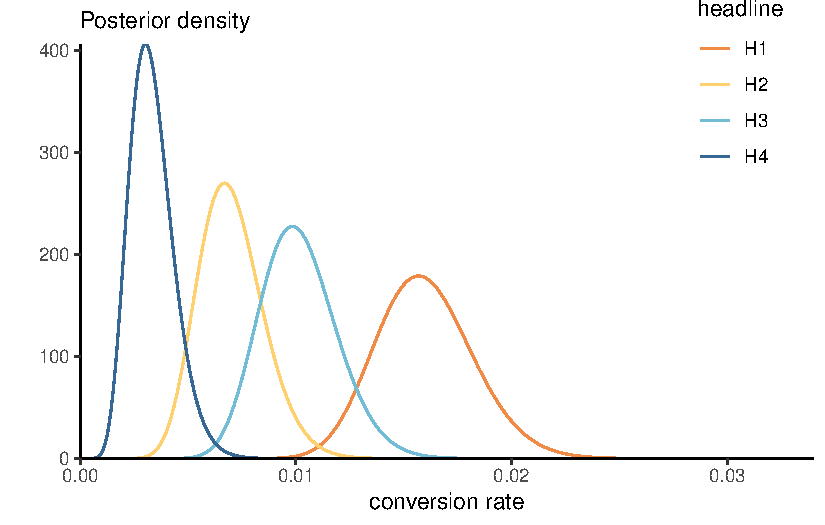
\includegraphics{priors_files/figure-pdf/fig-upworthy-1.pdf}

}

\caption{\label{fig-upworthy}Gamma posterior for conversion rate of the
different Upworthy Sesame Street headline.}

\end{figure}

We can visualize the posterior distributions. In this context, the large
sample size lead to the dominance of the likelihood contribution
\(p(Y_i \mid \lambda_i) \sim \mathsf{Pois}(n_i\lambda_i)\) relative to
the prior. We can see there is virtually no overlap between different
rates for headers H1 (preferred) relative to H4 (least favorable). The
probability that the conversion rate for Headline 3 is higher than
Headline 1 can be approximated by simulating samples from both
posteriors and computing the proportion of times one is larger: we get
1.7\% for \texttt{H3} relative to \texttt{H1}, indicating a clear
preference for the first headline \texttt{H1}.

\end{example}

\begin{example}[Should you phrase your headline as a
question?]\protect\hypertarget{exm-poisson-upworthy-question}{}\label{exm-poisson-upworthy-question}

We can also consider aggregate records for Upworthy, as Alexander
(\protect\hyperlink{ref-Alexander:2023}{2023}) did. The
\texttt{upworthy\_question} database contains a balanced sample of all
headlines where at least one of the choices featured a question, with at
least one alternative statement. Whether a headline contains a question
or not is determined by querying for the question mark. We consider
aggregated counts for all such headlines, with the \texttt{question}
factor encoding whether there was a question, \texttt{yes} or
\texttt{no}. For simplicity, we treat the number of views as fixed, but
keep in mind that A/B tests are often sequential experiments with a
stopping rule.\footnote{The stopping rule means that data stops being
  collected once there is enough evidence to determine if an option is
  more suitable, or if a predetermined number of views has been reached.}

We model first the rates using a Poisson regression; the corresponding
frequentist analysis would include an offset to account for differences
in views. If \(\lambda_{j}\) \((j=1, 2)\) are the average rate for each
factor level (yes and no), then
\(\mathsf{E}(Y_{ij}/n_{ij}) = \lambda_j\). In the frequentist setting,
we can fit a simple Poisson generalized linear regression model with an
offset term and a binary variable.

\begin{Shaded}
\begin{Highlighting}[]
\FunctionTok{data}\NormalTok{(upworthy\_question, }\AttributeTok{package =} \StringTok{"hecbayes"}\NormalTok{)}
\NormalTok{poismod }\OtherTok{\textless{}{-}} \FunctionTok{glm}\NormalTok{(}
\NormalTok{  clicks }\SpecialCharTok{\textasciitilde{}} \FunctionTok{offset}\NormalTok{(}\FunctionTok{log}\NormalTok{(impressions)) }\SpecialCharTok{+}\NormalTok{ question, }
  \AttributeTok{family =} \FunctionTok{poisson}\NormalTok{(}\AttributeTok{link =} \StringTok{"log"}\NormalTok{),}
  \AttributeTok{data =}\NormalTok{ upworthy\_question)}
\FunctionTok{coef}\NormalTok{(poismod)}
\end{Highlighting}
\end{Shaded}

\begin{verbatim}
(Intercept)  questionno 
-4.51264669  0.07069677 
\end{verbatim}

The coefficients represent the difference in log rate (multiplicative
effect) relative to the baseline rate, with an increase of 6.3 percent
when the headline does not contain a question. A likelihood ratio test
can be performed by comparing the deviance of the null model
(intercept-only), indicating strong evidence that including question
leads to significatively different rates. This is rather unsurprising
given the enormous sample sizes.

Consider instead a Bayesian analysis with conjugate prior: we model
separately the rates of each group (question or not). Suppose we think
apriori that the click-rate is on average 1\%, with a standard deviation
of 2\%, with no difference between questions or not. For a
\(\mathsf{Gamma}(\alpha, \beta)\) prior, this would translate, using
moment matching, into a rate of
\(\beta = 0.04 = \mathsf{Var}_0(\lambda_j)/\mathsf{E}_0(\lambda_j)\) and
a shape of \(\alpha = 2.5\) (\(j=1, 2\)). If \(\lambda_{j}\) is the
average rate for each factor level (yes and no), then
\(\mathsf{E}(Y_{ij}/n_{ij}) = \lambda_j\) so the log likelihood is
proportional, as a function of \(\lambda_1\) and \(\lambda_2\), to
\begin{align*}
\ell(\boldsymbol{\lambda}; \boldsymbol{y}, \boldsymbol{n}) \stackrel{\boldsymbol{\lambda}}{\propto} \sum_{i=1}^n \sum_{j=1}^2 y_{ij}\log \lambda_j - \lambda_jn_{ij}
\end{align*} and we can recognize that the posterior for \(\lambda_i\)
is gamma with shape \(\alpha + \sum_{i=1}^n y_{ij}\) and rate
\(\beta + \sum_{i=1}^n n_{ij}.\) For inference, we thus only need to
select hyperparameters and calculate the total number of clicks and
impressions per group. We can then consider the posterior difference
\(\lambda_1 - \lambda_2\) or, to mimic the Poisson multiplicative model,
of the ratio \(\lambda_1/\lambda_2\). The former suggests very small
differences, but one must keep in mind that rates are also small. The
ratio, shown in the right-hand panel of
Figure~\ref{fig-hist-difference_rates}, gives a more easily
interpretable portrait that is in line with the frequentist analysis.

\begin{figure}[ht!]

{\centering 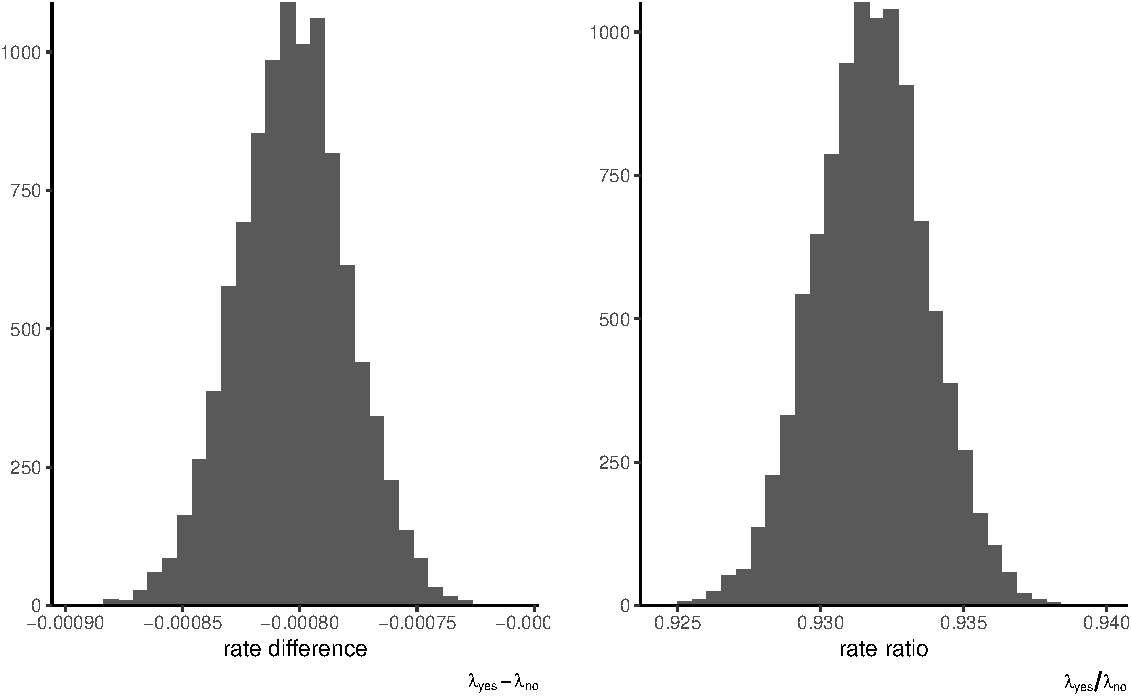
\includegraphics{priors_files/figure-pdf/fig-hist-difference_rates-1.pdf}

}

\caption{\label{fig-hist-difference_rates}Histograms of posterior
summaries for differences (left) and rates (right) based on 1000
simulations from the independent gamma posteriors.}

\end{figure}

To get an approximation to the posterior mean of the ratio
\(\lambda_1/\lambda_2,\) it suffices to draw independent observations
from their respective posterior, compute the ratio and take the sample
mean of those draws. We can see that the sampling distribution of the
ratio is nearly symmetrical, so we can expect Wald intervals to perform
well should one be interested in building confidence intervals. This is
however hardly surprising given the sample size at play.

\end{example}

\begin{example}[Conjugate prior for Gaussian mean with known
variance]\protect\hypertarget{exm-conjugatepriors-normal}{}\label{exm-conjugatepriors-normal}

Consider an \(n\) simple random sample of independent and identically
distributed Gaussian variables with mean \(\mu\) and standard deviation
\(\sigma\), denoted \(Y_i \sim \mathsf{Norm}(\mu, \sigma^2)\). We pick a
Gaussian prior for the location parameter,
\(\mu \sim \mathsf{Norm}(\nu, \tau^2)\) where we assume \(\mu, \tau\)
are fixed hyperparameter values. For now, we consider only inference for
\(p(\mu \mid \sigma)\): discarding any term that is not a function of
\(\mu\), the conditional posterior is \begin{align*}
p(\mu \mid \sigma) &\propto \exp\left\{ -\frac{1}{2\sigma^2}\sum_{i=1}^n (y_{i}-\mu)^2\right\} \exp\left\{-\frac{1}{2\tau^2}(\mu - \nu)^2\right\}
\\&\propto \exp\left\{\left(\frac{\sum_{i=1}^n y_{i}}{\sigma^2} + \frac{\nu}{\tau^2}\right)\mu - \left( \frac{n}{2\sigma^2} +\frac{1}{2\tau^2}\right)\mu^2\right\}.
\end{align*} The log of the posterior density conditional on \(\sigma\)
is quadratic in \(\mu\), it must be a Gaussian distribution truncated
over the positive half line. This can be seen by completing the square
in \(\mu\), or by comparing this expression to the density of
\(\mathsf{Norm}(\mu, \sigma^2)\), \begin{align*}
f(x; \mu, \sigma) \stackrel{\mu}{\propto} \exp\left(-\frac{1}{2 \sigma^2}\mu^2 + \frac{x}{\sigma^2}\mu\right)
\end{align*} we can deduce by matching mean and variance that the
conditional posterior \(p(\mu \mid \sigma)\) is Gaussian with reciprocal
variance (precision) \(n/\sigma^2 + 1/\tau^2\) and mean
\((n\overline{y}\tau^2 + \nu \sigma^2)/(n\tau^2 + \sigma^2)\). The
precision is an average of that of the prior and data, but assigns more
weight to the latter, which increases linearly with the sample size
\(n\). Likewise, the posterior mean is a weighted average of prior and
sample mean, with weights proportional to the relative precision.

\end{example}

The exponential family is quite large;
\href{https://citeseerx.ist.psu.edu/doc/10.1.1.157.5540}{Fink (1997)
\emph{A Compendium of Conjugate Priors}} gives multiple examples of
conjugate priors and work out parameter values.

In general, unless the sample size is small and we want to add expert
opinion, we may wish to pick an \emph{uninformative prior}, i.e., one
that does not impact much the outcome. For conjugate models, one can
often show that the relative weight of prior parameters (relative to the
random sample likelihood contribution) becomes negligible by
\href{https://en.wikipedia.org/wiki/Conjugate_prior}{investigating their
relative weights}.

\hypertarget{uninformative-priors}{%
\section{Uninformative priors}\label{uninformative-priors}}

\begin{definition}[Proper
prior]\protect\hypertarget{def-properprior}{}\label{def-properprior}

We call a prior function \emph{proper} if it's integral is finite over
the parameter space; such prior function automatically leads to a valid
posterior.

\end{definition}

The best example of prior priors arise from probability density
function. We can still employ this rule for improper priors: for
example, taking \(\alpha, \beta \to 0\) in the beta prior leads to a
prior proportional to \(x^{-1}(1-x)^{-1}\), the integral of which
diverges on the unit interval \([0,1]\). However, as long as the number
of success and the number of failures is larger than 1, meaning
\(k \geq 1, n-k \geq 1\), the posterior distribution would be proper,
i.e., integrable. To find the posterior, normalizing constants are also
superfluous.

Many uninformative priors are flat, or proportional to a uniform on some
subset of the real line and therefore improper. It may be superficially
tempting to set a uniform prior on a large range to ensure posterior
property, but the major problem is that a flat prior may be informative
in a different parametrization, as the following example suggests.

Gelman et al. (\protect\hyperlink{ref-Gelman:2013}{2013}) uses the
following taxonomy for various levels of prior information:
uninformative priors are generally flat or uniform priors with
\(p(\beta) \propto 1\), vague priors are typically nearly flat even if
proper, e.g., \(\beta \sim \mathsf{Norm}(0, 100)\), weakly informative
priors provide little constraints \(\beta \sim \mathsf{Norm}(0, 10)\),
and informative prior are typically application-specific, but constrain
the ranges. Uninformative and vague priors are generally not recommended
unless they are known to give valid posterior inference and the amount
of information from the likelihood is high.

\begin{example}[Transformation of flat prior for
scales]\protect\hypertarget{exm-scaleflatprior}{}\label{exm-scaleflatprior}

Consider the parameter \(\log(\tau) \in \mathbb{R}\) and the prior
\(p( \log \tau) \propto 1\). If we reparametrize the model in terms of
\(\tau\), the new prior (including the Jacobian of the transformation)
is \(\tau^{-1}\)

\end{example}

Some priors are standard and widely used. In location scale families
with location \(\nu\) and scale \(\tau\), the density is such that
\begin{align*}
f(x; \nu, \tau) =  \frac{1}{\tau} f\left(\frac{x - \nu}{\tau}\right), \qquad \nu \in \mathbb{R}, \tau >0.
\end{align*} We thus wish to have a prior so that
\(p(\tau) = c^{-1}p(\tau/c)\) for any scaling \(c>0\), whence it follows
that \(p(\tau) \propto \tau^{-1}\), which is uniform on the log scale.

The priors \(p(\nu) \propto 1\) and \(p(\tau) \propto \tau^{-1}\) are
both improper but lead to location and scale invariance, hence that the
result is the same regardless of the units of measurement.

One criticism of the Bayesian approach is the arbitrariness of prior
functions. However, the role of the prior is often negligible in large
samples (consider for example the posterior of exponential families with
conjugate priors). Moreover, the likelihood is also chosen for
convenience, and arguably has a bigger influence on the conclusion. Data
fitted using a linear regression model seldom follow Gaussian
distributions conditionally, in the same way that the linearity is a
convenience (and first order approximation).

\begin{definition}[Jeffrey's
prior]\protect\hypertarget{def-jeffreys}{}\label{def-jeffreys}

In single parameter models, taking a prior function for \(\theta\)
proportional to the square root of the determinant of the information
matrix, \(p(\theta) \propto |\imath(\theta)|^{1/2}\) yields a prior that
is invariant to reparametrization, so that inferences conducted in
different parametrizations are equivalent.\footnote{The Fisher
  information is linear in the sample size for independent and
  identically distributed data so we can derive the result for \(n=1\)
  without loss of generality.}

To see this, consider a bijective transformation
\(\theta \mapsto \vartheta\). Under the reparametrized model and
suitable regularity conditions\footnote{Using Bartlett's identity;
  Fisher consistency can be established using the dominated convergence
  theorem.}, the chain rule implies that \begin{align*}
i(\vartheta) &= - \mathsf{E} \left(\frac{\partial^2 \ell(\vartheta)}{\partial^2 \vartheta}\right)
\\&= - \mathsf{E}\left(\frac{\partial^2 \ell(\theta)}{\partial \theta^2}\right) \left( \frac{\mathrm{d} \theta}{\mathrm{d} \vartheta} \right)^2 + \mathsf{E}\left(\frac{\partial \ell(\theta)}{\partial \theta}\right) \frac{\mathrm{d}^2 \theta}{\mathrm{d} \vartheta^2}
\end{align*} Since the score has mean zero,
\(\mathsf{E}\left\{\partial \ell(\theta)/\partial \theta\right\}=0\) and
the rightmost term vanishes. We can thus relate the Fisher information
in both parametrizations, with \begin{align*}
\imath^{1/2}(\vartheta) = \imath^{1/2}(\theta) \left| \frac{\mathrm{d} \theta}{\mathrm{d} \vartheta} \right|,
\end{align*} implying invariance.

In multiparameter models, the system isn't invariant to
reparametrization if we consider the determinant of the Fisher
information.

\end{definition}

\begin{example}[Jeffrey's prior for the binomial
distribution]\protect\hypertarget{exm-jeffreysbinom}{}\label{exm-jeffreysbinom}

Consider the binomial distribution \(\mathsf{Bin}(1, \theta)\) with
density
\(f(y; \theta) \propto \theta^y(1-\theta)^{1-y}\mathsf{I}_{\theta \in [0,1]}\).
The negative of the second derivative of the log likelihood with respect
to \(p\) is
\[\jmath(\theta) = - \partial^2 \ell(\theta; y) / \partial \theta^2 = y/\theta^2 + (1-y)/(1-\theta)^2\]
and since \(\mathsf{E}(Y)=\theta\), the Fisher information is
\[\imath(\vartheta) = \mathsf{E}\{\jmath(\theta)\}=1/\theta + 1/(1-\theta) = 1/\{\theta(1-\theta)\}\]
Jeffrey's prior is thus
\(p(\theta) \propto \theta^{-1/2}(1-\theta)^{-1/2}\), a conjugate Beta
prior \(\mathsf{Beta}(0.5,0.5)\).

\end{example}

\hypertarget{exer-jeffreysnormal}{}
\hypertarget{jeffreys-prior-for-the-normal-distribution}{%
\section{Jeffrey's prior for the normal
distribution}\label{jeffreys-prior-for-the-normal-distribution}}

Check that for the Gaussian distribution
\(\mathsf{Norm}(\mu, \sigma^2)\), the Jeffrey's prior obtained by
treating each parameter as fixed in turn, are \(p(\mu) \propto 1\) and
\(p(\sigma) \propto 1/\sigma\), which also correspond to the default
uninformative priors for location-scale families.

\begin{example}[Jeffrey's prior for the Poisson
distribution]\protect\hypertarget{exm-jeffreyspoisson}{}\label{exm-jeffreyspoisson}

The Poisson distribution with
\(\ell(\lambda) \propto -\lambda + y\log \lambda\), with second
derivative
\(-\partial^2 \ell(\lambda)/\partial \lambda^2 = y/\lambda^2\). Since
the mean of the Poisson distribution is \(\lambda\), the Fisher
information is \(\imath(\lambda) = \lambda^{-1}\) and Jeffrey's prior is
\(\lambda^{-1/2}\).

\end{example}

\hypertarget{informative-priors}{%
\section{Informative priors}\label{informative-priors}}

One strength of the Bayesian approach is the capability of incorporating
expert and domain-based knowledge through priors. Often, these will take
the form of moment constraints, so one common way to derive a prior is
to perform moment matching to related ellicited quantities with moments
of the prior distribution. It may be easier to set priors on a different
scale than those of the observations, as Example~\ref{exm-colestawn}
demonstrates.

\begin{example}[Gamma quantile difference priors for extreme value
distributions]\protect\hypertarget{exm-colestawn}{}\label{exm-colestawn}

The generalized extreme value distribution arises as the limiting
distribution for the maximum of \(m\) independent observations from some
common distribution \(F\). The \(\mathsf{GEV}(\mu, \sigma, \xi)\)
distribution is a location-scale with distribution function
\begin{align*}
F(x) = \exp\left[ - \left\{1+\xi(x-\mu)/\sigma\right\}^{-1/\xi}_{+}\right]
\end{align*} where \(x_{+} = \max\{0, x\}\).

Inverting the distribution function yields the quantile function
\begin{align*}
Q(p) \mu + \sigma \frac{(-\log p)^{-\xi}-1}{\xi}
\end{align*}

In environmental data, we often model annual maximum. Engineering
designs are often specified in terms of the \(k\)-year return levels,
defined as the quantile of the annual maximum exceeded with probability
\(1/k\) in any given year. Using a \(\mathsf{GEV}\) for annual maximum,
Coles and Tawn (\protect\hyperlink{ref-Coles.Tawn:1996}{1996}) proposed
modelling annual daily rainfall and specifying a prior on the quantile
scale \(q_1 < q_2 < q_3\) for tail probabilities \(p_1> p_2 > p_3\). To
deal with the ordering constraints, gamma priors are imposed on the
differences \(q_1 - o \sim \mathsf{Gamma}(\alpha_1, \beta_1)\),
\(q_2 - q_1 \sim \mathsf{Gamma}(\alpha_2, \beta_2)\) and
\(q_3-q_2 \sim \mathsf{Gamma}(\alpha_3, \beta_3)\), where \(o\) is the
lower bound of the support. The prior is thus of the form

\begin{align*}
p(\boldsymbol{q}) \propto q_1^{\alpha_1-1}\exp(-\beta_1 q_1) \prod_{i=2}^3 (q_i-q_{i-1})^{\alpha_i-1} \exp\{\beta_i(q_i-q_{i-1})\}.
\end{align*} where \(0 \leq q_1 \leq q_2 \leq q_3\). The fact that these
quantities refer to moments or risk estimates which practitioners often
must compute as part of regulatory requirements makes it easier to
specify sensible values for hyperparameters.

As illustrating example, consider maximum daily cumulated rainfall in
Abisko, Sweden. The time series spans from 1913 until December 2014; we
compute the 102 yearly maximum, which range from 11mm to 62mm, and fit a
generalized extreme value distribution to these.

For the priors, suppose an expert elicits quantiles of the 10, 50 and
100 years return levels; say 30mm, 45mm and 70mm, respectively, for the
median and likewise 40mm, 70mm and 120mm for the 90\% percentile of the
return levels. We can compute the differences and calculate the
parameters of the gamma distribution through moment-matching: this gives
roughly a shape of \(\alpha_1=18.27\) and \(\beta_1=0.6\), etc.
Figure~\ref{fig-gev-colestawn-quant-prior} shows the transfer from the
prior predictive to the posterior distribution. The prior is much more
dispersed and concentrated on the tail, which translates in a less
peaked posterior than using a weakly informative prior (dotted line):
the mode of the latter is slightly to the left and with lower density in
the tail.

\begin{figure}[ht!]

{\centering 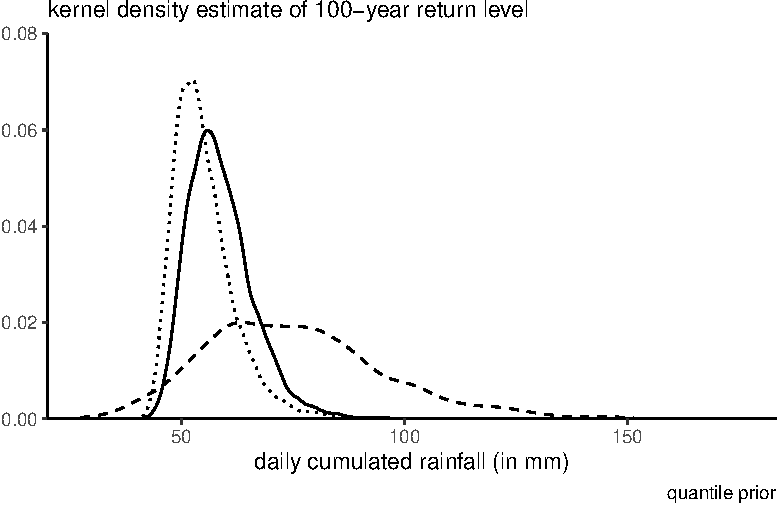
\includegraphics{priors_files/figure-pdf/fig-gev-colestawn-quant-prior-1.pdf}

}

\caption{\label{fig-gev-colestawn-quant-prior}Kernel density estimates
of draws from the posterior distribution of 100 year return levels with
a Coles--Tawn quantile prior (full line) and from the corresponding
prior predictive (dashed). The dotted line gives the posterior
distribution for a maximum domain information prior on the shape with
improper priors on location and scale.}

\end{figure}

\end{example}

What would you do if we you had prior information from different
sources? One way to combine these is through a mixture: given \(M\)
different prior distributions \(p_m(\boldsymbol{\theta})\), we can
assign each a positive weight \(w_m\) to form a mixture of experts prior
through the linear combination
\[ p(\boldsymbol{\theta}) \propto \sum_{m=1}^M w_m p_m(\boldsymbol{\theta})\]

\hypertarget{penalized-complexity-priors}{%
\subsection{Penalized complexity
priors}\label{penalized-complexity-priors}}

Oftentimes, there will be a natural family of prior density to impose on
some model component, \(p(\boldsymbol{\theta} \mid \zeta)\), with
hyperparameter \(\zeta\). The flexibility of the underlying construction
leads itself to overfitting. Penalized complexity priors
(\protect\hyperlink{ref-Simpson:2017}{Simpson et al. 2017}) aim to
palliate this by penalizing models far away from a simple baseline
model, which correspond to a fixed value \(\zeta_0\). The prior will
favour the simpler parsimonious model the more prior mass one places on
\(\zeta_0\), which is in line with Occam's razor principle.

To construct a penalized-complexity prior, we compute the
Kullback--Leibler divergence between the model
\(p_\zeta \equiv p(\boldsymbol{\theta} \mid \zeta)\) relative to the
baseline with \(\zeta_0\),
\(p_0 \equiv p(\boldsymbol{\theta} \mid \zeta_0)\); the
Kullback--Leibler divergence is

\[
\mathsf{KL}(p_\zeta \Vert\, p_0)=\int p_\zeta \log\left(\frac{p_\zeta}{p_0}\right) \mathrm{d} \boldsymbol{\theta}.
\] The distance between the prior densities is then set to
\(d(\zeta) = \{2\mathsf{KL}(p_\zeta \mid\mid p_0)\}^{1/2}\). which is
zero at the model with \(\zeta_0\). The PC prior then constructs an
exponential prior on the distance scale, which after back-transformation
gives
\(p(\zeta \mid \lambda) = \lambda\exp(-\lambda d(\zeta)) \left| {\partial d(\zeta)}/{\partial \zeta}\right|\).
To choose \(\lambda\), the authors recommend elicitation of a pair
\((U, \alpha)\) such that \(\Pr(\lambda > U)=\alpha\).

\begin{example}[Penalized complexity prior for random effects
models]\protect\hypertarget{exm-pcprior-randomeffect}{}\label{exm-pcprior-randomeffect}

Simpson et al. (\protect\hyperlink{ref-Simpson:2017}{2017}) give the
example of a Gaussian prior for random effects \(\boldsymbol{\alpha}\),
of the form
\(\boldsymbol{\alpha} \mid \zeta \sim \mathsf{Norm}_J(\boldsymbol{0}_J, \zeta^2 \mathbf{I}_J)\)
where \(\zeta_0=0\) corresponds to the absence of random
subject-variability. The penalized complexity prior for the scale
\(\zeta\) is then an exponential with rate \(\lambda\),\footnote{Possibly
  truncated above if the support of \(\zeta\) has a finite upper bound.}
with density \(p(\zeta \mid \lambda) = \lambda \exp(-\lambda \zeta)\).
Using the recommendation for setting \(\lambda\), we get that
\(\lambda = -\ln(\alpha/U)\) and this can be directly interpreted in
terms of standard deviation of \(\zeta\); simulation from the prior
predictive may also be used for calibration.

\end{example}

\begin{example}[Penalized complexity prior for autoregressive model of
order
1]\protect\hypertarget{exm-pcprior-arorder}{}\label{exm-pcprior-arorder}

Sørbye and Rue (\protect\hyperlink{ref-Sorbye.Rue:2017}{2017}) derive
penalized complexity prior for the Gaussian stationary AR(1) model with
autoregressive parameter \(\phi \in (-1,1)\), where
\(Y_t \mid Y_{t-1}, \phi, \sigma^2 \sim \mathsf{Norm}(\phi Y_{t-1}, \sigma^2)\).
There are two based models that could be of interest: one with
\(\phi=0\), corresponding to a memoryless model with no autocorrelation,
and a static mean \(\phi=1\) for no change in time; note that the latter
is not stationary. For the former, the penalized complexity prior is
\begin{align*}
p(\phi \mid \lambda) = \frac{\lambda}{2} \exp\left[-\lambda \left\{-\ln(1-\phi^2)\right\}^{1/2}\right] \frac{|\phi|}{(1-\phi^2)\left\{-\ln(1-\phi^2)\right\}^{1/2}}.
\end{align*} One can set \(\lambda\) by considering plausible values by
relating the parameter to the variance of the one-step ahead forecast
error.

\end{example}

Gaussian components are widespread: not only for linear regression
models, but more generally for the specification of random effects that
capture group-specific effects, residuals spatial or temporal
variability. In the Bayesian paradigm, there is no difference between
fixed effects \(\boldsymbol{\beta}\) and the random effect parameters:
both are random quantities that get assigned priors, but we will treat
these priors differently.

The reason why we would like to use a penalized complexity prior for a
random effect, say \(\alpha_j \sim \mathsf{Norm}(0, \zeta^2)\), is
because we don't know a prior if there is variability between groups.
The inverse gamma prior for \(\zeta\),
\(\zeta \sim \mathsf{InvGamma}(\epsilon, \epsilon)\) does not have a
mode at zero unless it is improper with \(\epsilon \to 0\). Generally,
we want our prior for the variance to have significant probability
density at the null \(\zeta=0\). The penalized complexity prior is not
the only sensible choice. Posterior inference is unfortunately sensitive
to the value of \(\epsilon\) in hierarchical models when the random
effect variance is close to zero, and more so when there are few levels
for the groups since the relative weight of the prior relative to that
of the likelihood contribution is then large.

\begin{example}[Student-t prior for variance
components]\protect\hypertarget{exm-random-effect-variance}{}\label{exm-random-effect-variance}

Gelman (\protect\hyperlink{ref-Gelman:2006}{2006}) recommends a
Student-\(t\) distribution truncated below at \(0\), with low degrees of
freedom. The rationale for this choice comes from the simple two level
model with \(n_j\) independent in each group \(j=1, \ldots, J\): for
observation \(i\) in group \(j\), \begin{align*}
Y_{ij} &\sim \mathsf{Norm}(\mu + \alpha_j, \sigma^2),\\
\alpha_j &\sim \mathsf{Norm}(0, \tau^2_\alpha), 
\end{align*} The conditionally conjugate prior
\(p(\tau \mid \boldsymbol{\alpha}, \mu, \sigma)\) is inverse gamma.
Standard inference with this parametrization is however complicated,
because there is strong dependence between parameters.

To reduce this dependence, one can add a parameter, taking
\(\alpha_j = \xi \eta_j\) and \(\tau_\alpha=|\xi|\tau_{\eta}\); the
model is now overparametrized. Suppose
\(\eta_j \sim \mathsf{Norm}(0, \tau^2_\eta)\) and consider the
likelihood conditional on \(\mu, \eta_j\): we have that
\((y_{ij} - \mu)/\eta_j \sim \mathsf{Norm}(\xi, \sigma^2/\eta_j)\) so
conditionally conjugate priors for \(\xi\) and \(\tau_\eta\) are
respectively Gaussian and inverse gamma. This translates into a prior
distribution for \(\tau_\alpha\) which is that of the absolute value of
a noncentral Student-\(t\) with location, scale and degrees of freedom
\(\nu\). If we set the location to zero, the prior puts high mass at the
origin, but is heavy tailed with polynomial decay. We recommend to set
degrees of freedom so that the variance is heavy-tailed, e.g.,
\(\nu=3\). While this prior is not conjugate, it compares favorably to
the \(\mathsf{IGa}(\epsilon, \epsilon)\).

\end{example}

\begin{example}[Poisson random effect
models]\protect\hypertarget{exm-randomeffects}{}\label{exm-randomeffects}

We consider data from an experimental study conducted at Tech3Lab on
road safety. In Brodeur et al.
(\protect\hyperlink{ref-Brodeur:2021}{2021}), 31 participants were asked
to drive in a virtual environment; the number of road violation was
measured for different type of distractions (phone notification, phone
on speaker, texting and smartwatch). The data are balanced, with each
participant exposed to each task exactly once.

We model the data using a Poisson mixed model to measure the number of
violations, \texttt{nviolation}, with a fixed effect for \texttt{task},
which captures the type of distraction, and a random effect for
participant \texttt{id}. The hierarchical model fitted for individual
\(i\) \((i=1, \ldots, 34)\) and distraction type \(j\)
\((j=1, \ldots, 4)\) is \begin{align*}
Y_{ij} &\sim \mathsf{Pois}\{\mu = \exp(\beta_{j} + \alpha_i)\},\\
\beta_j &\sim \mathsf{Norm}(0, 100), \\
\alpha_i &\sim \mathsf{Norm}(0, \kappa^2), \\
\kappa &\sim \mathsf{St}_{+}(3).
\end{align*} so observations are conditionally independent given
hyperparameters \(\boldsymbol{\alpha}\) and \(\boldsymbol{\beta}\).

In frequentist statistics, there is a distinction made in mixed-effect
models between parameters that are treated as constants, termed fixed
effects and corresponding in this example to \(\boldsymbol{\beta}\), and
random effects, equivalent to \(\boldsymbol{\alpha}\). There is no such
distinction in the Bayesian paradigm, except perhaps for the choice of
prior.

We can look at some of posterior distribution of the 31 random effects
(here the first five individuals) and the fixed effect parameters
\(\boldsymbol{\beta}\), plus the variance of the random effect
\(\kappa\): there is strong evidence that the latter is non-zero,
suggesting strong heterogeneity between individuals. The distraction
which results in the largest number of violation is texting, while the
other conditions all seem equally distracting on average (note that
there is no control group with no distraction to compare with, so it is
hard to draw conclusions).

\begin{figure}[ht!]

{\centering 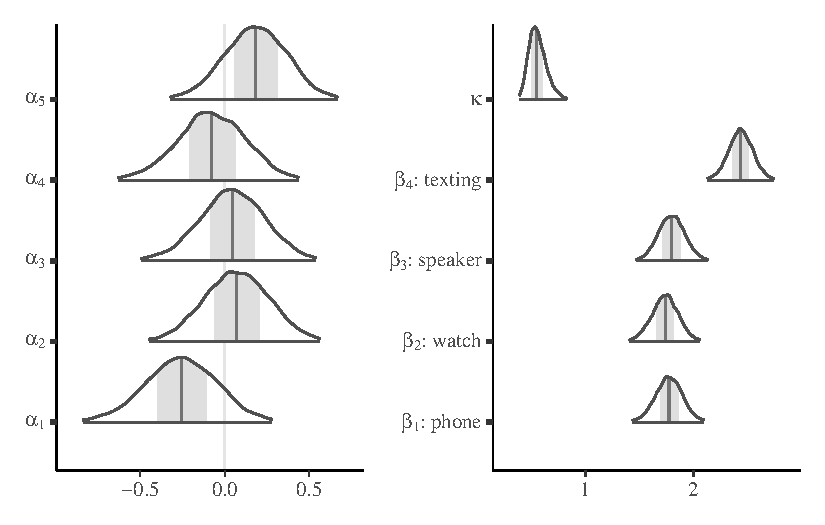
\includegraphics{priors_files/figure-pdf/fig-post-dist-poisson-mixed-1.pdf}

}

\caption{\label{fig-post-dist-poisson-mixed}Posterior density plots with
50\% credible intervals and median value for the random effects of the
first five individuals (left) and the fixed effects and random effect
variance (right).}

\end{figure}

\end{example}

\hypertarget{sensitivity-analysis}{%
\section{Sensitivity analysis}\label{sensitivity-analysis}}

Do priors matter? The answer to that question depends strongly on the
model, and how much information the data provides about hyperparameters.
While this question is easily answered in conjugate models (the relative
weight of hyperparameters relative to data can be derived from the
posterior parameters), it is not so simple in hierarchical models, where
the interplay between prior distributions is often more intricate. To
see the impact, one often has to rely on doing several analyses with
different values fr the prior and see the sensitivity of the conclusions
to these changes, for example by considering a vague prior or modifying
the parameters values (say halving or doubling). If the changes are
immaterial, then this provides reassurance that our analyses are robust.

\begin{example}[]\protect\hypertarget{exm-sensitivity-poisson-mixed}{}\label{exm-sensitivity-poisson-mixed}

To check the sensitivity of the conclusion, we revisit the modelling of
the \texttt{smartwatch} experiment data using a Poisson regression and
compare four priors: a uniform prior truncated to \([0, 10]\), an
inverse gamma \(\mathsf{InvGamma}(0.01, 0.01)\) prior, a penalized
complexity prior such that the 0.95 percentile of the scale is 5,
corresponding to \(\mathsf{Exp}(0.6)\). Since each distraction type
appears 31 times, there is plenty of information to reliably estimate
the dispersion \(\kappa\) of the random effects \(\alpha\): the
different density plots in Figure~\ref{fig-sensitivity} are virtually
indistinguishable from one another. This is perhaps unsurprising given
the large number of replicates, and the significant variability between
groups.

\begin{figure}[ht!]

{\centering 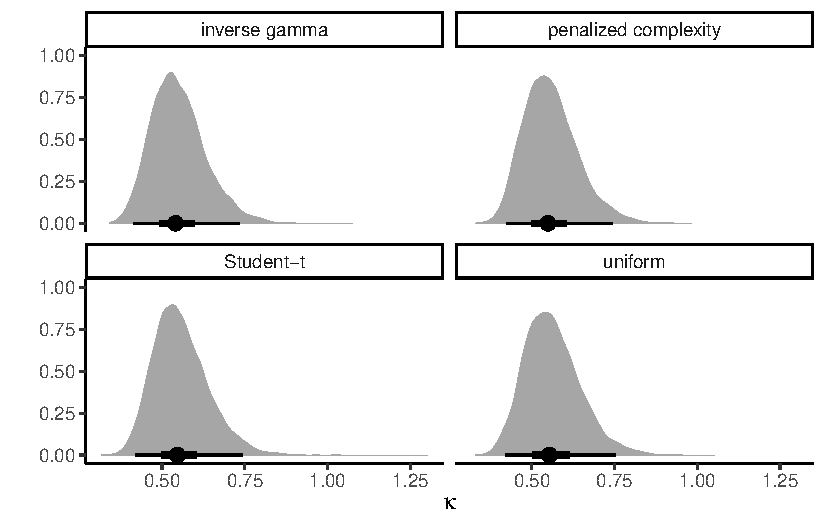
\includegraphics{priors_files/figure-pdf/fig-sensitivity-1.pdf}

}

\caption{\label{fig-sensitivity}Posterior density of the scale of the
random effects with uniform, inverse gamma, penalized complexity and
folded Student-t with three degrees of freedom. The circle denotes the
median and the bars the 50\% and 95\% percentile credible intervals.}

\end{figure}

\end{example}

\bookmarksetup{startatroot}

\hypertarget{simulation-based-inference}{%
\chapter{Simulation-based inference}\label{simulation-based-inference}}

There are two major approaches to handling the problem of the unknown
normalizing constant: deterministic and stochastic approximations. The
former includes Laplace and nested Laplace approximations, variational
methods and expectation propagation. This chapter covers the latter,
stochastic approximations, and focuses on implementation of basic Markov
chain Monte Carlo algorithms. The simulation algorithms circumvent the
need to calculate the normalizing constant of the posterior entirely. We
present several examples of implementations, several tricks for tuning
and diagnostics of convergence.

\hypertarget{monte-carlo-methods}{%
\section{Monte Carlo methods}\label{monte-carlo-methods}}

Consider a target distribution with finite expected value: think of the
posterior of some model of interest, or some functional thereof. The law
of large numbers guarantees that, if we can draw observations from our
target distribution, then the sample average will converge to the
expected value of that distribution, as the sample size becomes larger
and larger, provided the expectation is finite.

We can thus compute the probability of any event or the expected value
of any (integrable) function by computing sample averages; the cost to
pay for this generality is randomness.

Specifically, suppose we are interested in the average
\(\mathsf{E}\{g(X)\}\) of \(X_i \sim F\) for some function \(g\).

\begin{example}[]\protect\hypertarget{exm-expectation-demo}{}\label{exm-expectation-demo}

Consider \(X \sim \mathsf{Gamma}(\alpha, \beta)\), a gamma distribution
with shape \(\alpha\) and rate \(\beta\). We can compute the probability
that \(X < 1\) easily by Monte Carlo since
\(\Pr(X <1) = \mathsf{E}\{\mathrm{I}(X<1)\}\) and this means we only
need to compute the proportion of draws less than one. We can likewise
compute the mean \(g(x) = x\) or variance.

Suppose we have drawn a Monte Carlo sample of size \(B\). If the
function \(g(\cdot)\) is square integrable,\footnote{Meaning
  \(\mathsf{E}\{g^2(X)\}<\infty\), so the variance of \(g(X)\) exists.}
with variance \(\sigma^2_g\), then a central limit theorem applies. In
large samples and for independent observations, our Monte Carlo average
\(\widehat{\mu}_g = B^{-1}\sum_{b=1}^B g(X_i)\) has variance
\(\sigma^2_g/B\). We can approximate the unknown variance \(\sigma^2_g\)
by it's empirical counterpart.\footnote{By contrasts, if data are
  identically distributed but not independent, care is needed}. Note
that, while the variance decreases linearly with \(B\), the choice of
\(g\) impacts the speed of convergence: we can compute
\[\sigma^2_g =\Pr(X \leq 1)\{1-\Pr(X \leq 1)\}=0.0434\] (left) and
\(\sigma^2_g=\alpha/\beta^2=1/8\) (middle plot).

Figure~\ref{fig-monte-carlo-path} shows the empirical trace plot of the
Monte Carlo average (note the \(\sqrt{B}\) \(x\)-axis scale!) as a
function of the Monte Carlo sample size \(B\) along with 95\% Wald-based
confidence intervals (gray shaded region),
\(\widehat{\mu}_g \pm 1.96 \times \sigma_g/\sqrt{B}\). We can see that
the `likely region' for the average shrinks with \(B\).

What happens if our function is not integrable? The right-hand plot of
Figure~\ref{fig-monte-carlo-path} shows empirical averages of
\(g(x) = x^{-1}\), which is not integrable if \(\alpha < 1\). We can
compute the empirical average, but the result won't converge to any
meaningful quantity regardless of the sample size. The large jumps are
testimonial of this.

\begin{figure}[ht!]

{\centering 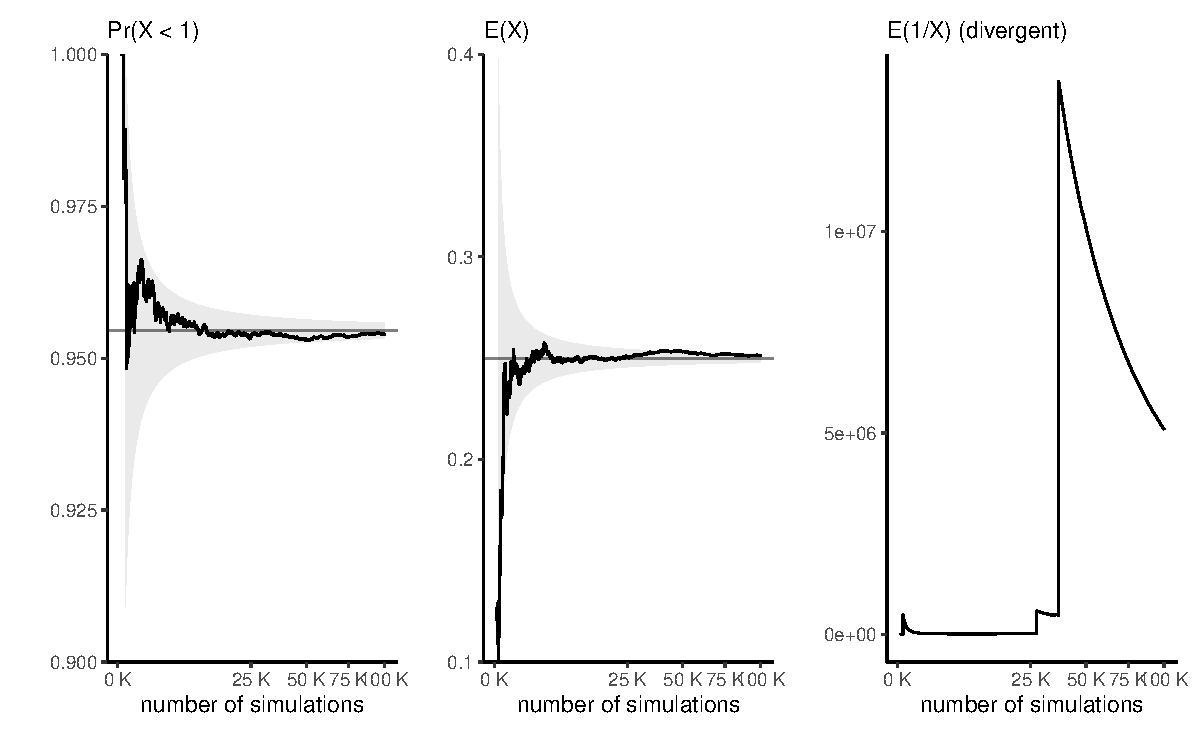
\includegraphics{mcmc_files/figure-pdf/fig-monte-carlo-path-1.pdf}

}

\caption{\label{fig-monte-carlo-path}Running mean trace plots for
\(g(x)=\mathrm{I}(x<1)\) (left), \(g(x)=x\) (middle) and \(g(x)=1/x\)
(right) for a Gamma distribution with shape 0.5 and rate 2, as a
function of the Monte Carlo sample size.}

\end{figure}

\end{example}

We have already used Monte Carlo methods to compute posterior quantities
of interest in conjugate models. Outside of models with conjugate
priors, the lack of closed-form expression for the posterior precludes
inference. Indeed, calculating the posterior probability of an event, or
posterior moments, requires integration of the normalized posterior
density and thus knowledge of the marginal likelihood. It is seldom
possible to sample independent and identically distributed (iid) samples
from the target, especially if the model is high dimensional: rejection
sampling and the ratio of uniform method are examples of Monte Carlo
methods which can be used to generate iid draws.

\begin{proposition}[Rejection
sampling]\protect\hypertarget{prp-rejection-sampling}{}\label{prp-rejection-sampling}

Rejection sampling (also termed accept-reject algorithm) samples from a
random vector with density \(p(\cdot)\) by drawing candidates from a
proposal with density \(q(\cdot)\) with nested support,
\(\mathrm{supp}(p) \subseteq \mathrm{supp}(q)\). The density
\(q(\cdot)\) must be such that
\(p(\boldsymbol{\theta}) \leq C q(\boldsymbol{\theta})\) for
\(C \geq 1\) for all values of \(\boldsymbol{\theta}\) in the support of
\(p(\cdot)\). A proof can be found in Devroye
(\protect\hyperlink{ref-Devroye:1986}{1986}, Theorem 3.1)

\begin{enumerate}
\def\labelenumi{\arabic{enumi}.}
\tightlist
\item
  Generate \(\boldsymbol{\theta}^{\star}\) from the proposal with
  density \(q\) and \(U \sim \mathsf{U}(0,1)\)
\item
  Compute the ratio
  \(R \gets p(\boldsymbol{\theta}^{\star})/ q(\boldsymbol{\theta}^{\star})\).
\item
  If \(R \geq CU\), return \(\boldsymbol{\theta}\), else go back to step
  1.
\end{enumerate}

\end{proposition}

\begin{figure}[ht!]

{\centering 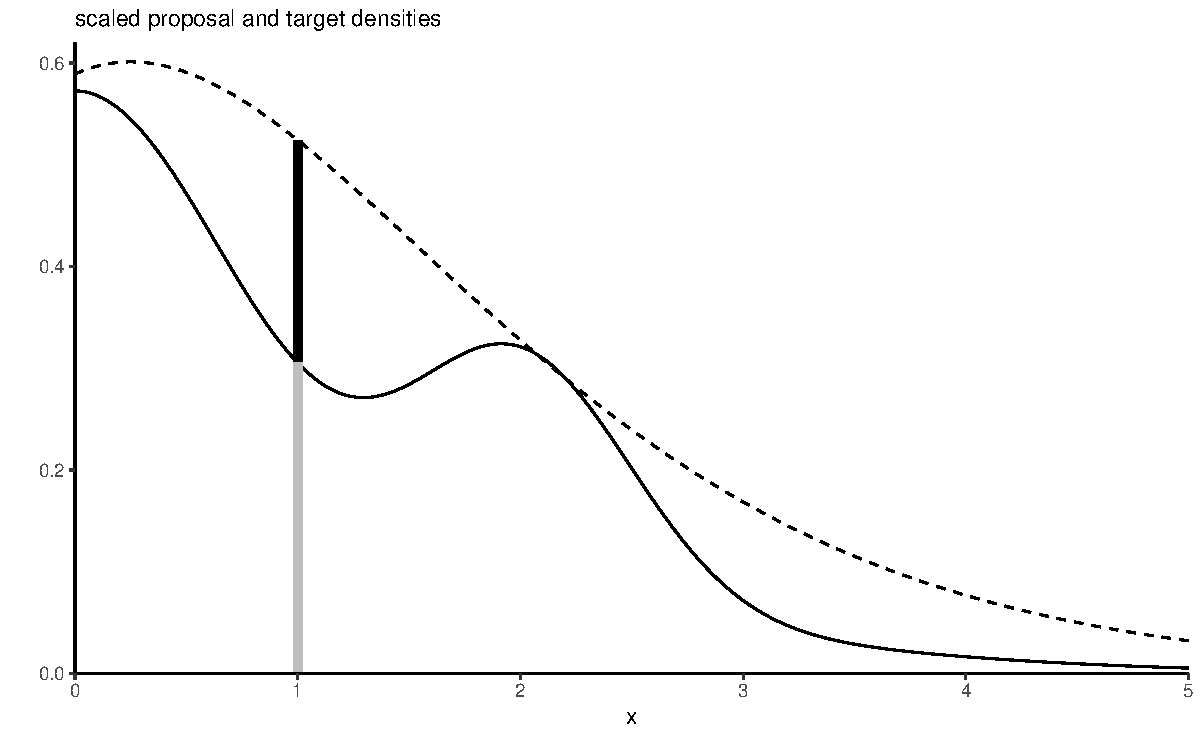
\includegraphics{mcmc_files/figure-pdf/fig-acceptreject-1.pdf}

}

\caption{\label{fig-acceptreject}Target density (full) and scaled
proposal density (dashed): the vertical segment at \(x=1\) shows the
percentage of acceptance for a uniform slice under the scaled proposal,
giving an acceptance ratio of 0.58.}

\end{figure}

Rejection sampling requires the proposal \(q\) to have a support at
least as large as that of \(p\) and resemble closely the density. It
should be chosen so that the upper bound \(C\) is as sharp as possible
and close to 1. The dominating density \(q\) must have heavier tails
than the density of interest. The expected number of simulations needed
to accept one proposal is \(C.\) Finally, for the method to be useful,
we need to be able to simulate easily and cheaply from the proposal. The
optimal value of \(C\) is
\(C = \sup_{\boldsymbol{\theta}} p(\boldsymbol{\theta}) / q(\boldsymbol{\theta})\).
This quantity may be obtained by numerical optimization, by finding the
mode of the ratio of the log densities if the maximum is not known
analytically.

\begin{example}[Truncated Gaussian
distribution]\protect\hypertarget{exm-accept-reject-truncated}{}\label{exm-accept-reject-truncated}

Consider the problem of sampling from a Gaussian distribution
\(Y \sim \mathsf{Norm}(\mu, \sigma^2)\) truncated in the interval
\([a, b],\) which has density \begin{align*}
f(x; \mu, \sigma, a, b) = \frac{1}{\sigma}\frac{\phi\left(\frac{x-\mu}{\sigma}\right)}{\Phi\{(b-\mu)/\sigma\}-\Phi\{(a-\mu)/\sigma\}}.
\end{align*} where \(\phi(\cdot), \Phi(\cdot)\) are respectively the
density and distribution function of the standard Gaussian distribution.

Since the Gaussian is a location-scale family, we can reduce the problem
to sampling \(X\) from a standard Gaussian truncated on
\(\alpha = (a-\mu)/\sigma\) and \(\beta = (b-\mu)/\sigma\) and back
transform the result as \(Y = \mu + \sigma X\).

A crude accept-reject sampling algorithm would consider sampling from
the same untruncated distribution with density
\(g(X) = \sigma^{-1}\phi\{(x-\mu)/\sigma\}\), and the acceptance ratio
is \(C^{-1}=\{\Phi(\beta) - \Phi(\alpha)\}\). We thus simply simulate
points from the Gaussian and accept any that falls within the bounds.

\begin{Shaded}
\begin{Highlighting}[]
\CommentTok{\# Standard Gaussian truncated on [0,1]}
\NormalTok{candidate }\OtherTok{\textless{}{-}} \FunctionTok{rnorm}\NormalTok{(}\FloatTok{1e5}\NormalTok{)}
\NormalTok{trunc\_samp }\OtherTok{\textless{}{-}}\NormalTok{ candidate[candidate }\SpecialCharTok{\textgreater{}=} \DecValTok{0} \SpecialCharTok{\&}\NormalTok{ candidate }\SpecialCharTok{\textless{}=} \DecValTok{1}\NormalTok{]}
\CommentTok{\# Acceptance rate}
\FunctionTok{length}\NormalTok{(trunc\_samp)}\SpecialCharTok{/}\FloatTok{1e5}
\end{Highlighting}
\end{Shaded}

\begin{verbatim}
[1] 0.34242
\end{verbatim}

\begin{Shaded}
\begin{Highlighting}[]
\CommentTok{\# Theoretical acceptance rate}
\FunctionTok{pnorm}\NormalTok{(}\DecValTok{1}\NormalTok{)}\SpecialCharTok{{-}}\FunctionTok{pnorm}\NormalTok{(}\DecValTok{0}\NormalTok{)}
\end{Highlighting}
\end{Shaded}

\begin{verbatim}
[1] 0.3413447
\end{verbatim}

We can of course do better: if we consider a random variable with
distribution function \(F,\) but truncated over the interval \([a,b],\)
then the resulting distribution function is
\[\frac{F(x) - F(a)}{F(b)-F(a)}, \qquad a \leq x \leq b,\] and we can
invert this expression to get the quantile function of the truncated
variable in terms of the distribution function \(F\) and the quantile
function \(F^{-1}\) of the original untruncated variable.

For the Gaussian, this gives \begin{align*}
X \sim \Phi^{-1}\left[\Phi(\alpha) + \{\Phi(\beta)-\Phi(\alpha)\}U\right]
\end{align*} for \(U \sim \mathsf{U}(0,1)\). Although the quantile and
distribution functions of the Gaussian, \texttt{pnorm} and
\texttt{qnorm} in \textbf{R}, are very accurate, this method will fail
for rare event simulation because it will return \(\Phi(x) = 0\) for
\(x \leq -39\) and \(\Phi(x)=1\) for \(x \geq 8.3\), implying that
\(a \leq 8.3\) for this approach to work
(\protect\hyperlink{ref-LEcuyer.Botev:2017}{Botev and L'Écuyer 2017}).

Consider the problem of simulating events in the right tail for a
standard Gaussian where \(a > 0\); Marsaglia's method
(\protect\hyperlink{ref-Devroye:1986}{Devroye 1986, 381}), can be used
for that purpose. Write the density of the Gaussian as
\(f(x) = \exp(-x^2/2)/c_1\), where
\(c_1 = \int_{a}^{\infty}\exp(-z^2/2)\mathrm{d} z\), and note that
\[c_1f(x) \leq \frac{x}{a}\exp\left(-\frac{x^2}{2}\right)= a^{-1}\exp\left(-\frac{a^2}{2}\right)g(x), \qquad x \geq a;\]
where \(g(x)\) is the density of a Rayleigh variable shifted by \(a\),
which has distribution function \(G(x) = 1-\exp\{(a^2-x^2)/2\}\) for
\(x \geq a\). We can simulate such a random variate \(X\) through the
inversion method. The constant \(C= \exp(-a^2/2)(c_1a)^{-1}\) approaches
1 quickly as \(a \to \infty\).

The accept-reject thus proceeds with

\begin{enumerate}
\def\labelenumi{\arabic{enumi}.}
\tightlist
\item
  Generate a shifted Rayleigh above \(a\),
  \(X \gets \{a^2 - 2\log(U)\}^{1/2}\) for \(U \sim \mathsf{U}(0,1)\)
\item
  Accept \(X\) if \(XV \leq a\), where \(V \sim \mathsf{U}(0,1)\).
\end{enumerate}

Should we wish to obtain samples on \([a,b]\), we could instead propose
from a Rayleigh truncated above at \(b\)
(\protect\hyperlink{ref-LEcuyer.Botev:2017}{Botev and L'Écuyer 2017}).

\begin{Shaded}
\begin{Highlighting}[]
\NormalTok{a }\OtherTok{\textless{}{-}} \FloatTok{8.3}
\NormalTok{niter }\OtherTok{\textless{}{-}}\NormalTok{ 1000L}
\NormalTok{X }\OtherTok{\textless{}{-}} \FunctionTok{sqrt}\NormalTok{(a}\SpecialCharTok{\^{}}\DecValTok{2} \SpecialCharTok{+} \DecValTok{2}\SpecialCharTok{*}\FunctionTok{rexp}\NormalTok{(niter))}
\NormalTok{samp }\OtherTok{\textless{}{-}}\NormalTok{ X[}\FunctionTok{runif}\NormalTok{(niter)}\SpecialCharTok{*}\NormalTok{X }\SpecialCharTok{\textless{}=}\NormalTok{ a]}
\end{Highlighting}
\end{Shaded}

\end{example}

For a given candidate density \(g\) which has a heavier tail than the
target, we can resort to numerical methods to compute the mode of the
ratio \(f/g\) and obtain the bound \(C\); see Albert
(\protect\hyperlink{ref-Albert:2009}{2009}), Section 5.8 for an
insightful example.

\begin{proposition}[Ratio of uniform
method]\protect\hypertarget{prp-ratio-uniform}{}\label{prp-ratio-uniform}

The ratio-of-uniform method
(\protect\hyperlink{ref-Kinderman.Monahan:1977}{Kinderman and Monahan
1977}; \protect\hyperlink{ref-Wakefield:1991}{Wakefield, Gelfand, and
Smith 1991}) is a variant of accept-reject used to draw samples from a
unnormalized density \(f(\boldsymbol{\theta})\) for
\(\boldsymbol{\theta} \in \boldsymbol{\Theta} \subseteq \mathbb{R}^d\).
For some \(r \geq 0\), consider the set \begin{align*}
\mathcal{C}_r = \left\{ (u_0, \ldots, u_d): 0 < u_0 \leq \left[f(u_1/u_0^r, \ldots, u_d/u_0^r)\right]^{\frac{1}{rd+1}}\right\}.
\end{align*} If we can generate \(u_0, \ldots, u_d\) uniformly over
\(\mathcal{C}_R\), then the draws \((u_1/u_0^r, \ldots, u_d/u_0^r)\) are
from the normalized density \(f\). Rejection sampling is used to obtain
uniform draws over \(\mathcal{C}_r\) under some conditions on the
density and marginal moments. See
\href{https://paulnorthrop.github.io/rust/articles/rust-a-vignette.html}{the
\texttt{rust} package vignette} for technical details and examples. Like
with other accept-reject algorithms, the acceptance rate of the proposal
goes down with the dimension of the problem.

\end{proposition}

\begin{example}[]\protect\hypertarget{exm-rust}{}\label{exm-rust}

The ratio-of-uniform algorithm was used in
Example~\ref{exm-loss-extremes} to generate draws from the posterior. We
illustrate below the \texttt{rust} package with a user-specified prior
and posterior. We fit a generalized Pareto distribution
\(Y \sim \mathsf{GP}(\sigma, \xi)\) to exceedances above 10 millions
krones to the \texttt{danish} fire insurance data, using a truncated
maximal data information prior
\(p(\sigma, \xi) \propto \sigma^{-1}\exp(-\xi+1)\mathrm{I}(\xi > -1)\).

\begin{Shaded}
\begin{Highlighting}[]
\FunctionTok{data}\NormalTok{(danish, }\AttributeTok{package =} \StringTok{"evir"}\NormalTok{)}
\CommentTok{\# Extract threshold exceedances}
\NormalTok{exc }\OtherTok{\textless{}{-}}\NormalTok{ danish[danish }\SpecialCharTok{\textgreater{}} \DecValTok{10}\NormalTok{] }\SpecialCharTok{{-}} \DecValTok{10}
\CommentTok{\# Create a function for the log prior}
\NormalTok{logmdiprior }\OtherTok{\textless{}{-}} \ControlFlowTok{function}\NormalTok{(par, ...)\{}
  \ControlFlowTok{if}\NormalTok{(}\FunctionTok{isTRUE}\NormalTok{(}\FunctionTok{any}\NormalTok{(par[}\DecValTok{1}\NormalTok{] }\SpecialCharTok{\textless{}=} \DecValTok{0}\NormalTok{, par[}\DecValTok{2}\NormalTok{] }\SpecialCharTok{\textless{}} \SpecialCharTok{{-}}\DecValTok{1}\NormalTok{)))\{}
    \FunctionTok{return}\NormalTok{(}\SpecialCharTok{{-}}\ConstantTok{Inf}\NormalTok{)}
\NormalTok{  \}}
  \SpecialCharTok{{-}}\FunctionTok{log}\NormalTok{(par[}\DecValTok{1}\NormalTok{]) }\SpecialCharTok{{-}}\NormalTok{ par[}\DecValTok{2}\NormalTok{]}
\NormalTok{\}}
\CommentTok{\# Same for log likelihood, assuming independent data}
\NormalTok{loglik\_gp }\OtherTok{\textless{}{-}} \ControlFlowTok{function}\NormalTok{(par, }\AttributeTok{data =}\NormalTok{ exc, ...)\{}
  \ControlFlowTok{if}\NormalTok{(}\FunctionTok{isTRUE}\NormalTok{(}\FunctionTok{any}\NormalTok{(par[}\DecValTok{1}\NormalTok{] }\SpecialCharTok{\textless{}=} \DecValTok{0}\NormalTok{, par[}\DecValTok{2}\NormalTok{] }\SpecialCharTok{\textless{}} \SpecialCharTok{{-}}\DecValTok{1}\NormalTok{)))\{}
    \FunctionTok{return}\NormalTok{(}\SpecialCharTok{{-}}\ConstantTok{Inf}\NormalTok{)}
\NormalTok{  \}}
  \FunctionTok{sum}\NormalTok{(mev}\SpecialCharTok{::}\FunctionTok{dgp}\NormalTok{(}\AttributeTok{x =}\NormalTok{ data, }\AttributeTok{scale =}\NormalTok{ par[}\DecValTok{1}\NormalTok{], }\AttributeTok{shape =}\NormalTok{ par[}\DecValTok{2}\NormalTok{], }\AttributeTok{log =} \ConstantTok{TRUE}\NormalTok{))}
\NormalTok{\}}
\NormalTok{logpost }\OtherTok{\textless{}{-}} \ControlFlowTok{function}\NormalTok{(par, ...)\{}
  \FunctionTok{logmdiprior}\NormalTok{(par) }\SpecialCharTok{+} \FunctionTok{loglik\_gp}\NormalTok{(par)}
\NormalTok{\}}
\CommentTok{\# Sampler using ratio{-}of{-}uniform method}
\NormalTok{ru\_output }\OtherTok{\textless{}{-}}\NormalTok{ rust}\SpecialCharTok{::}\FunctionTok{ru}\NormalTok{(}
  \AttributeTok{logf =}\NormalTok{ logpost,  }\CommentTok{\# log posterior function}
  \AttributeTok{n =} \DecValTok{10000}\NormalTok{, }\CommentTok{\# number of posterior draws}
  \AttributeTok{d =} \DecValTok{2}\NormalTok{, }\CommentTok{\# dimension of the parameter vector}
  \AttributeTok{init =}\NormalTok{ mev}\SpecialCharTok{::}\FunctionTok{fit.gpd}\NormalTok{(danish, }\AttributeTok{thresh =} \DecValTok{10}\NormalTok{)}\SpecialCharTok{$}\NormalTok{par,}
  \AttributeTok{lower =} \FunctionTok{c}\NormalTok{(}\DecValTok{0}\NormalTok{, }\SpecialCharTok{{-}}\DecValTok{1}\NormalTok{))}
\DocumentationTok{\#\# Acceptance rate }
\CommentTok{\# ru\_output$pa}
\DocumentationTok{\#\# Posterior samples}
\NormalTok{postsamp }\OtherTok{\textless{}{-}}\NormalTok{ ru\_output}\SpecialCharTok{$}\NormalTok{sim\_vals}
\end{Highlighting}
\end{Shaded}

Even without modification, the acceptance rate is 52\%, which is quite
efficient in the context. The generalized Pareto approximation suggests
a very heavy tail: values of \(\xi \geq 1\) correspond to distributions
with infinite first moment, and those with \(\xi \geq 1/2\) to infinite
variance.

\begin{figure}[ht!]

{\centering 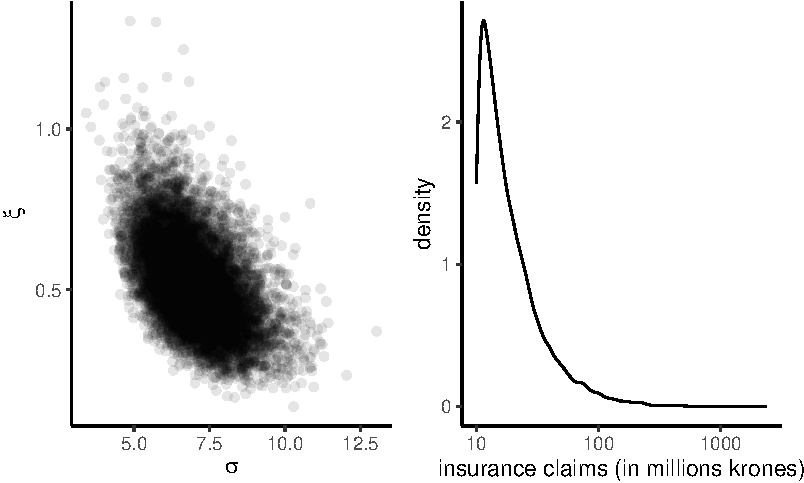
\includegraphics{mcmc_files/figure-pdf/fig-danish-rou-1.pdf}

}

\caption{\label{fig-danish-rou}Scatterplot of posterior samples from the
generalized Pareto model applied to Danish fire insurance losses above
10 millions krones, with maximal data information prior (left) and
posterior predictive density on log scale (right).}

\end{figure}

\end{example}

\hypertarget{markov-chain-monte-carlo}{%
\section{Markov chain Monte Carlo}\label{markov-chain-monte-carlo}}

Plain ordinary Monte Carlo is great, but few algorithms are generic
enough to be useful in complex high-dimensional problems. Instead, we
will construct a Markov chain with a given invariant distribution
corresponding to the posterior. Markov chain Monte Carlo methods
generate correlated draws that will target the posterior under suitable
conditions.\footnote{While we won't focus on the fine prints of the
  contract, there are conditions for validity and these matter!}

Before going forward with algorithms for sampling, we introduce some
terminology that should be familiar to people with a background in time
series analysis.

\begin{definition}[Stationarity and Markov
property]\protect\hypertarget{def-weak-stationarity}{}\label{def-weak-stationarity}

A stochastic (i.e., random) process is (weakly) stationary if the
distribution of \(\{X_1, \ldots, X_t\}\) is the same as that of
\(\{X_{n+1}, \ldots X_{t+n}\}\) for any value of \(n\) and given \(t\).

It is Markov if it satisfies the Markov property: given the current
state of the chain, the future only depends on the current state and not
on the past.

\end{definition}

\begin{example}[]\protect\hypertarget{exm-autoregressive-one}{}\label{exm-autoregressive-one}

Consider a first-order autoregressive process, or \(\mathsf{AR}(1)\), of
the form

\[Y_t = \mu + \phi(Y_{t-1} - \mu) + \varepsilon_t,\] where \(\phi\) is
the lag-one correlation, \(\mu\) the global mean and \(\varepsilon_t\)
is an iid innovation with mean zero and variance \(\sigma^2\). If
\(|\phi| < 1\), the process is stationary, and the variance does not
increase with \(t\). If innovations are Gaussian, we have
\[Y_t \mid Y_{t-1}=y_{t-1} \sim \mathsf{Norm}\{\mu(1-\phi)+ \phi y_{t-1}, \sigma^2\}.\]

The \(\mathsf{AR}(1)\) stationarity process \(Y_t\), marginally, has
mean \(\mu\) and unconditional variance \(\sigma^2/(1-\phi^2)\). The
\(\mathsf{AR}(1)\) process is first-order Markov since the conditional
distribution \(p(Y_t \mid Y_{t-1}, \ldots, Y_{t-p})\) equals
\(p(Y_t \mid Y_{t-1})\).

\end{example}

Autoregressive processes are not the only ones we can consider, although
their simplicity lends itself to analytic calculations. More generally,
for a correlated sequence, the variance of the stationary distribution
is \begin{align*}
\mathsf{Va}(Y_t) + 2 \sum_{k=1}^\infty \mathsf{Co}(Y_t, Y_{t-k})
\end{align*}

\begin{proposition}[Effective sample
size]\protect\hypertarget{prp-variance-clt}{}\label{prp-variance-clt}

Intuitively, a sample of correlated observations carries less
information than an independent sample of draws. If we want to compute
sample averages \(\overline{Y}_T=(Y_1+ \cdots + Y_T)/T\), the variance
will be \begin{align*}
\mathsf{Va}\left(\overline{Y}_T\right) = \frac{1}{T}\sum_{t=1}^T \mathsf{Va}(Y_t) + \frac{2}{T} \sum_{t=1}^{T-1}\sum_{s = t+1}^T \mathsf{Co}(Y_t, Y_s).
\end{align*}

In the independent case, the covariance is zero so we get the sum of
variances. If the process is stationary, the covariances at lag \(k\)
are the same regardless of the time index and the variance is some
constant, say \(\sigma^2\); this allows us to simplify calculations,
\begin{align*}
\mathsf{Va}(\overline{Y}_T) = \sigma^2 \left\{ 1 + \frac{2}{T}\sum_{t=1}^{T-1} (T-t) \mathsf{Cor}(Y_{T-k}, Y_{T})\right\}.
\end{align*} Denote the lag-\(k\) autocorrelation
\(\mathsf{Cor}(Y_{t}, Y_{t+k})\) by \(\gamma_k\). Under technical
conditions\footnote{Geometric ergodicity and existence of moments, among
  other things.}, a central limit theorem applies and we get an
asymptotic variance for the mean of \begin{align*}
\lim_{T \to \infty} T\mathsf{Va}\left(\overline{Y}_T\right) = \sigma^2 \left\{1+2\sum_{t=1}^\infty \gamma_t\right\}.
\end{align*} This statement holds only if we start with draws from the
stationary distribution, otherwise bets are off.

We need the \textbf{effective sample size} of our Monte Carlo averages
based on a Markov chain of length \(B\) to be sufficient for the
estimates to be meaningful. The effective sample size is, loosely
speaking, the equivalent number of observations if the marginal
posterior draws where independent and more formally
\begin{equation}\protect\hypertarget{eq-effective-sample-size}{}{
\mathsf{ESS} = \frac{B}{\left\{1+2\sum_{t=1}^\infty \gamma_t\right\}}
}\label{eq-effective-sample-size}\end{equation} where \(\gamma_t\) is
the lag \(t\) correlation. The relative effective sample size is simply
the fraction of the effective sample size over the Monte Carlo number of
replications: small values of \(\mathsf{ESS}/B\) indicate pathological
or inefficient samplers. If the ratio is larger than one, it indicates
the sample is superefficient (as it generates negatively correlated
draws).

In practice, we replace the unknown autocorrelations by sample estimates
and truncate the series in Equation~\ref{eq-effective-sample-size} at
the point where they become negligible --- typically when the
consecutive sum of two consecutive becomes negative; see Section 1.4 of
the
\href{https://mc-stan.org/docs/reference-manual/effective-sample-size.html}{Stan
manual} or Section 1.10.2 of Geyer
(\protect\hyperlink{ref-Geyer:2011}{2011}) for details.

\end{proposition}

\begin{example}[]\protect\hypertarget{exm-ar1-clt-variance}{}\label{exm-ar1-clt-variance}

The lag-\(k\) correlation of the stationary autoregressive process of
order 1 is \(\phi^k\), so summing the series gives an asymptotic
variance of \(\sigma^2(1+\phi)/(1-\phi)\). We can constrast that to the
variance of the stationary distribution for an independent sample, which
is \(\sigma^2/(1-\phi^2)\). The price to pay for having correlated
samples is inefficiency: the higher the autocorrelation, the larger the
variability of our mean estimators.

\begin{figure}[ht!]

{\centering 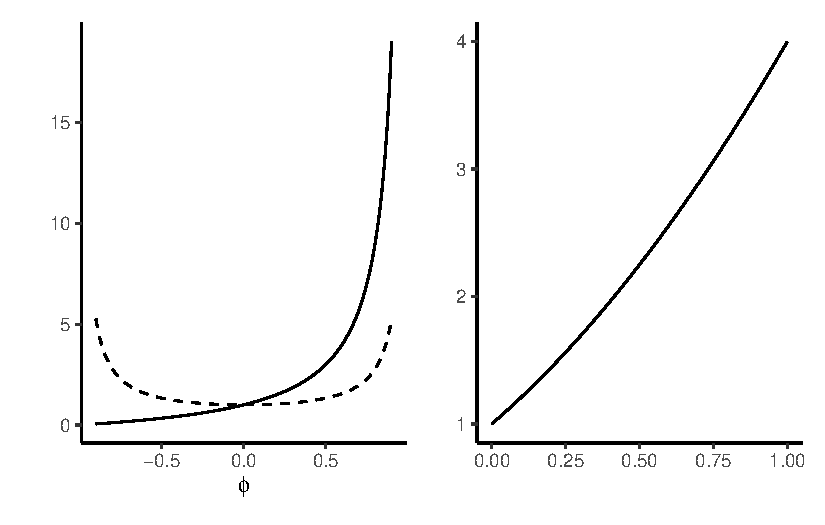
\includegraphics{mcmc_files/figure-pdf/fig-ar1-variance-1.pdf}

}

\caption{\label{fig-ar1-variance}Scaled asymptotic variance of the
sample mean for a stationary autoregressive first-order process with
unit variance (dashed) and a corresponding sample of independent
observations with the same marginal variance (full line). The plot on
the right gives the variance ratio for positive correlations.}

\end{figure}

We can see from Figure~\ref{fig-ar1-variance} that, when the
autocorrelation is positive (as will be the cause in all applications of
interest), we will suffer from variance inflation. To get the same
uncertainty estimates for the mean with an \(\mathsf{AR}(1)\) process
with \(\phi \approx 0.75\) than with an iid sample, we would need nine
times as many observations: this is the prize to pay.

\end{example}

\hypertarget{estimating-uncertainty-of-point-estimators-with-markov-chains}{%
\subsection{Estimating uncertainty of point estimators with Markov
chains}\label{estimating-uncertainty-of-point-estimators-with-markov-chains}}

With a simple random sample containing independent and identically
distributed observations, the standard error of the sample mean is
\(\sigma/\sqrt{n}\) and we can use the empirical standard deviation
\(\widehat{\sigma}\) to estimate the first term. For Markov chains, the
correlation prevents us from using this approach. The output of
the\texttt{coda} package are based on fitting a high order
autoregressive process to the Markov chain and using the formula of the
unconditional variance of the \(\mathsf{AR}(p)\) to obtain the central
limit theorem variance. An alternative method recommended by Geyer
(\protect\hyperlink{ref-Geyer:2011}{2011}) and implemented in his
\textbf{R} package \texttt{mcmc}, is to segment the time series into
batch, compute the means of each non-overlapping segment and use this
standard deviation with suitable rescaling to get the central limit
variance for the posterior mean. Figure~\ref{fig-mcmc-batchmean}
illustrate the method of batch means.

\begin{enumerate}
\def\labelenumi{\arabic{enumi}.}
\tightlist
\item
  Break the chain of length \(B\) (after burn in) in \(K\) blocks of
  size \(\approx K/B\).
\item
  Compute the sample mean of each segment. These values form a Markov
  chain and should be approximately uncorrelated.
\item
  Compute the standard deviation of the segments mean. Rescale by
  \(K^{-1/2}\) to get standard error of the global mean.
\end{enumerate}

Why does the approach work? If the chain samples from the stationary
distribution, all samples have the same mean. If we partition the sample
into long enough, the sample mean of each blocks should be roughly
independent (otherwise we could remove an overlapping portion). We can
then compute the empirical standard deviation of the estimators. We can
then compute the overall mean and use a scaling argument to relate the
variability of the global estimator with the variability of the means of
the smaller blocks.

\begin{figure}[ht!]

{\centering 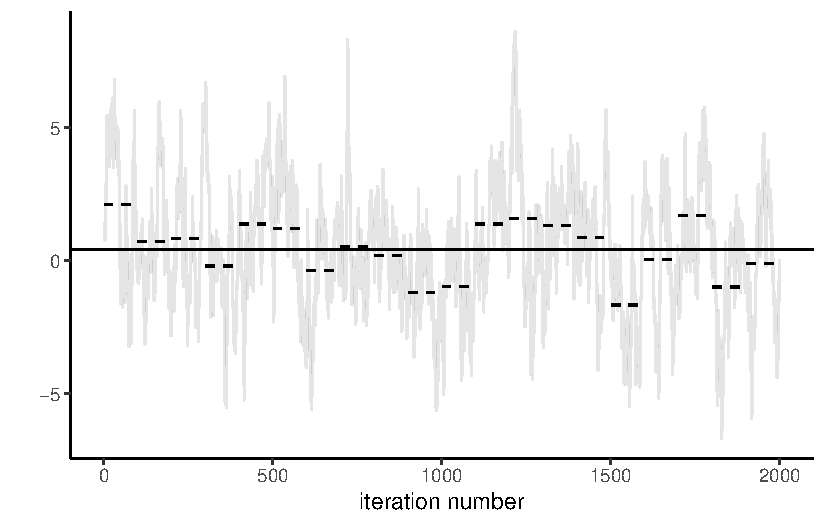
\includegraphics{mcmc_files/figure-pdf/fig-mcmc-batchmean-1.pdf}

}

\caption{\label{fig-mcmc-batchmean}Calculation of the standard error of
the posterior mean using the batch method.}

\end{figure}

When can we use output from a Markov chain in place of independent Monte
Carlo draws? The assumptions laid out in the ergodic theorem are that
the chain is irreducible and acyclic, ensuring that the chain has a
unique stationary distribution. The ergodic theorem is a result about
convergence of averages.

To make sense of these concepts, we consider a discrete Markov chain
over the integers \(1, 2, 3\). A discrete-time stochastic process is a
random sequences whose elements are part of some set, the state space,
here the integers. We can encode the probability of moving from one
state to the next via a transition matrix, whose rows contain the
probabilities of moving from one state to the next and thus sum to one.
We can run a Markov chain by sampling an initial state \(X_0\) at random
from \(\{1, \ldots, 5\}\) and then consider the transitions from the
conditional distribution, sampling \(p(X_t \mid X_{t-1})\). Because of
the Markov property, the history of the chain does not matter: we only
need to read the value \(i=X_{t-1}\) of the state and pick the \(i\)th
row of \(P_3\) to know the probability of the different moves from the
current state.

Irreducible means that the chain can move from anywhere to anywhere, so
it doesn't get stuck in part of the space forever. A transition matrix
such as \(P_1\) below describes a reducible Markov chain, because once
you get into state \(2\) or \(3\), you won't escape. With reducible
chains, the stationary distribution need not be unique, and so the
target would depend on the starting values.

Cyclical chains loop around and visit periodically a state: \(P_2\) is
an instance of transition matrix describing a chain that cycles from
\(1\) to \(3\), \(3\) to \(2\) and \(2\) to \(1\) every three iteration.
An acyclic chain is needed for convergence of marginals.

\[
P_1 = \begin{pmatrix}
0.5 & 0.3 & 0.2 \\
0 & 0.4 & 0.6 \\
0 & 0.5 & 0.5
\end{pmatrix}, 
\qquad 
P_2 = \begin{pmatrix}
0 & 0 & 1 \\
1 & 0 & 0 \\
0 & 1 & 0
\end{pmatrix}.
\]

If a chain is irreducible and aperiodic, it has a unique stationary
distribution and the limiting distribution of the Markov chain will
converge there. For example, we consider a transition \(P_3\) on
\(1, \ldots, 5\) defined as \[
P_3 = \begin{pmatrix}
\frac{2}{3} & \frac{1}{3} &  0 & 0 & 0 \\
\frac{1}{6} & \frac{2}{3} & \frac{1}{6} & 0 & 0 \\
0 & \frac{1}{6} & \frac{2}{3} & \frac{1}{6} & 0 \\
0 & 0 & \frac{1}{6} & \frac{2}{3} & \frac{1}{6} \\
0 & 0 & 0 &  \frac{1}{3}  & \frac{2}{3} \\
\end{pmatrix}
\] The stationary distribution is the value of the row vector
\(\boldsymbol{p}\), such that
\(\boldsymbol{p} = \boldsymbol{p}\mathbf{P}\) for transition matrix
\(\mathbf{P}\): we get \(\boldsymbol{p}_1=(0, 5/11, 6/11)\) for \(P_1\),
\((1/3, 1/3, 1/3)\) for \(P_2\) and \((1,2,2,2,1)/8\) for \(P_3\).

Figure~\ref{fig-discrete-markov-chain} shows the path of the walk and
the empirical proportion of the time spent in each state, as time
progress. Since the Markov chain has a unique stationary distribution,
we expect these to converge to it.

\begin{figure}[ht!]

{\centering 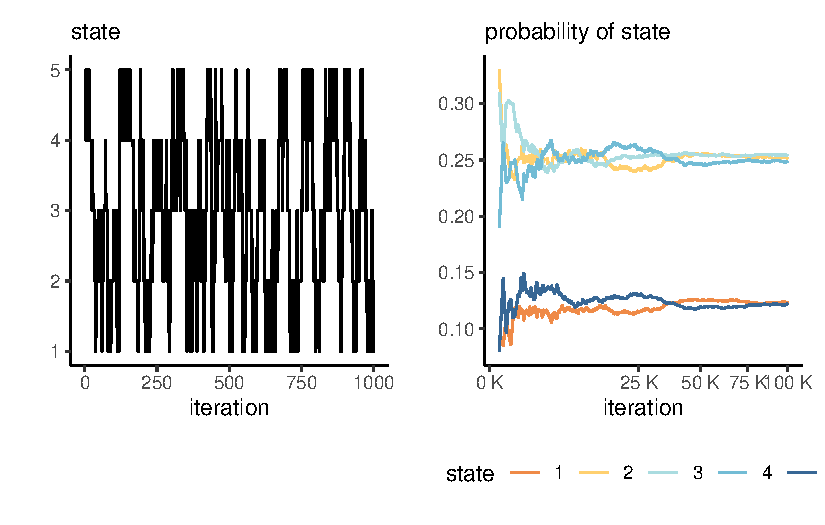
\includegraphics{mcmc_files/figure-pdf/fig-discrete-markov-chain-1.pdf}

}

\caption{\label{fig-discrete-markov-chain}Discrete Markov chain on
integers from 1 to 5, with transition matrix \(P_3\), with traceplot of
1000 first iterations (left) and running mean plots of sample proportion
of each state visited per 100 iterations (right).}

\end{figure}

\hypertarget{markov-chain-monte-carlo-algorithms}{%
\section{Markov chain Monte Carlo
algorithms}\label{markov-chain-monte-carlo-algorithms}}

The Markov chain Monte Carlo revolution in the 1990s made Bayesian
inference mainstream by allowing inference for models when only
approximations were permitted, and coincided with a time at which
computers became more widely available. The idea is to draw correlated
samples from a posterior via Markov chains, constructed to have the
posterior as invariant stationary distribution.

\begin{proposition}[Conjugate priors in the Bayesian linear
model]\protect\hypertarget{prp-conjugate-bayesian-linmod}{}\label{prp-conjugate-bayesian-linmod}

Consider a linear regression model with observation-specific mean
\(\mu_i = \mathbf{x}_i\boldsymbol{\beta}\) \((i=1,\ldots, n)\) with
\(\mathbf{x}_i\) the \(i\)th row of the \(n \times p\) model matrix
\(\mathbf{X}\).

Concatenating records,
\(\boldsymbol{Y} \sim \mathsf{No}_n(\mathbf{X}\boldsymbol{\beta}, \sigma^2 \mathbf{Q}_y^{-1})\),
for a known precision matrix \(\mathbf{Q}_y\), typically
\(\mathbf{I}_n\). To construct a conjugate joint prior for
\(p(\boldsymbol{\beta}, \sigma^2)\), we consider the sequential
formulation \begin{align*}
\boldsymbol{\beta} \mid \sigma^2 \sim \mathsf{No}_p(\boldsymbol{\nu}_\beta, \sigma^2 \mathbf{Q}^{-1}_\beta), \qquad \sigma^2 \sim \mathsf{IG}(\alpha,\beta)
\end{align*} where \(\mathsf{IG}\) denotes the inverse gamma
distribution\footnote{This simply means that the precision
  \(\sigma^{-2}\), the reciprocal of the variance, has a gamma
  distribution with shape \(\alpha\) and rate \(\beta\).}

The joint posterior is Gaussian-inverse gamma and can be factorized
\begin{align*}
p(\boldsymbol{\beta}, \sigma^2 \mid y) = p(\sigma^2 \mid y) p(\boldsymbol{\beta} \mid \sigma^2, y)
\end{align*} where
\(p(\sigma^2 \mid y) \sim \mathsf{IG}(\alpha^*, \beta^*)\) and
\(p(\boldsymbol{\beta} \mid \sigma^2, y) \sim \mathsf{No}_p(\mathbf{M}\boldsymbol{m}, \sigma^2\mathbf{M})\)
with \(\alpha^* = \alpha + n/2\),
\(\beta^*=\beta + 0.5 \boldsymbol{\nu}_\beta^\top \mathbf{Q}_\beta\boldsymbol{\nu}_\beta + \boldsymbol{y}^\top\boldsymbol{y} - \boldsymbol{m}^\top\mathbf{M}\boldsymbol{m}\),
\(\boldsymbol{m} = \mathbf{Q}_\beta \boldsymbol{\nu}_\beta + \mathbf{X}^\top \mathbf{Q}_y\boldsymbol{y}\)
and
\(\mathbf{M} = (\mathbf{Q}_\beta + \mathbf{X}^\top\mathbf{Q}_y\mathbf{X})^{-1};\)
the latter can be evaluated efficiently using
Shermann--Morrisson--Woodbury identity.

\end{proposition}

\hypertarget{metropolishastings-algorithm}{%
\subsection{Metropolis--Hastings
algorithm}\label{metropolishastings-algorithm}}

Named after Metropolis et al.
(\protect\hyperlink{ref-Metropolis:1953}{1953}), Hastings
(\protect\hyperlink{ref-Hastings:1970}{1970}), its relevance took a long
time to gain traction in the statistical community. The idea of the
Metropolis--Hastings algorithm is to construct a Markov chain targeting
a distribution \(p(\cdot)\).

\begin{proposition}[Metropolis--Hastings
algorithm]\protect\hypertarget{prp-metropolis}{}\label{prp-metropolis}

We consider from a density function \(p(\boldsymbol{\theta})\), known up
to a normalizing factor not depending on \(\boldsymbol{\theta}\). We use
a (conditional) proposal density
\(q(\boldsymbol{\theta} \mid \boldsymbol{\theta}^*)\) which has non-zero
probability over the support of \(p(\cdot)\), as transition kernel to
generate proposals.

The Metropolis--Hastings build a Markov chain starting from an initial
value \(\boldsymbol{\theta}_0\):

\begin{enumerate}
\def\labelenumi{\arabic{enumi}.}
\tightlist
\item
  draw a proposal value
  \(\boldsymbol{\theta}_t^{\star} \sim q(\boldsymbol{\theta} \mid \boldsymbol{\theta}_{t-1})\).
\item
  Compute the acceptance ratio
  \begin{equation}\protect\hypertarget{eq-metropolis-ratio}{}{
  R = \frac{p(\boldsymbol{\theta}_t^{\star})}{p(\boldsymbol{\theta}_{t-1})}\frac{q(\boldsymbol{\theta}_{t-1} \mid \boldsymbol{\theta}_t^{\star} )}{q(\boldsymbol{\theta}_t^{\star} \mid \boldsymbol{\theta}_{t-1})}
  }\label{eq-metropolis-ratio}\end{equation}
\item
  With probability \(\min\{R, 1\}\), accept the proposal and set
  \(\boldsymbol{\theta}_t \gets \boldsymbol{\theta}_t^{\star}\),
  otherwise set the value to the previous state,
  \(\boldsymbol{\theta}_t \gets \boldsymbol{\theta}_{t-1}\).
\end{enumerate}

\end{proposition}

The Metropolis--Hastings algorithm generates samples from the posterior
\(p(\boldsymbol{\theta} \mid \boldsymbol{y})\) if the Markov chain it
defines is reversible: we say it satisfies the \emph{detailed balance
condition} when the density of
\(\boldsymbol{\theta}_{t+1} \mid \boldsymbol{\theta}_{t}\), say
\(f(\boldsymbol{\theta}_{t+1} \mid \boldsymbol{\theta}_{t})\). Detailed
balance means \begin{align*}
f(\boldsymbol{\theta}_{t+1} \mid \boldsymbol{\theta}_{t})p(\boldsymbol{\theta}_{t} \mid \boldsymbol{y}) = f(\boldsymbol{\theta}_{t} \mid \boldsymbol{\theta}_{t+1})p(\boldsymbol{\theta}_{t+1} \mid \boldsymbol{y})
\end{align*} This guarantees that, if \(\boldsymbol{\theta}_{t}\) is
drawn from the posterior, then the left hand side is the joint density
of \((\boldsymbol{\theta}_{t}, \boldsymbol{\theta}_{t+1})\) and the
marginal distribution obtained by integrating over
\(\boldsymbol{\theta}_{t}\), \begin{align*}
&\int f(\boldsymbol{\theta}_{t+1} \mid \boldsymbol{\theta}_{t})p(\boldsymbol{\theta}_{t} \mid \boldsymbol{y})\mathrm{d} \boldsymbol{\theta}_{t}
\\&\quad = \int f(\boldsymbol{\theta}_{t} \mid \boldsymbol{\theta}_{t+1})p(\boldsymbol{\theta}_{t+1} \mid \boldsymbol{y})\mathrm{d} \boldsymbol{\theta}_{t} 
\\&\quad= p(\boldsymbol{\theta}_{t+1} \mid \boldsymbol{y})
\end{align*} and any draw from the posterior will generate a new
realization from the posterior. We also ensure that, provided the
starting value as non-zero probability under the posterior, the chain
will converge to the stationarity distribution (albeit perhaps slowly).

\begin{remark}[Interpretation of the algorithm]

If \(R>1\), the proposal has higher density and we always accept the
move. If the ratio is less than one, the proposal is in a lower
probability region, we accept the move with probability \(R\) and set
\(\boldsymbol{\theta}_{t}=\boldsymbol{\theta}^{\star}_t\); if we reject,
the Markov chain stays at the current value, which induces
autocorrelation. Since the acceptance probability depends only on the
density through ratios, we can work with unnormalized density functions
and this is what allows us, if our proposal density is the (marginal)
posterior of the parameter, to obtain approximate posterior samples
without having to compute the marginal likelihood.

\end{remark}

\begin{remark}[Blank run]

To check that the algorithm is well-defined, we can remove the log
likelihood component and run the algorithm: if it is correct, the
resulting draws should be drawn from the prior provided the latter is
proper (\protect\hyperlink{ref-Green:2001}{Green 2001, 55}).

\end{remark}

\begin{remark}[Symmetric proposals]

Suppose we generate a candidate sample \(\boldsymbol{\theta}_t^{\star}\)
from a symmetric distribution \(q(\cdot \mid \cdot)\) centered at
\(\boldsymbol{\theta}_{t-1}\), such as the random walk
\(\boldsymbol{\theta}_t^{\star} =\boldsymbol{\theta}_{t-1}+ Z\) where
\(Z\) has a symmetric distribution. Then, the proposal density ratio
cancels so need not be computed in the Metropolis ratio of
Equation~\ref{eq-metropolis-ratio}.

\end{remark}

\begin{remark}[Calculations]

In practice, we compute the log of the acceptance ratio, \(\ln R\), to
avoid numerical overflow. If our target is log posterior density, we
have \[
\ln \left\{\frac{p(\boldsymbol{\theta}_t^{\star})}{p(\boldsymbol{\theta}_{t-1})}\right\} = \ell(\boldsymbol{\theta}_t^{\star}) + \ln p(\boldsymbol{\theta}_t^{\star}) - \ell(\boldsymbol{\theta}_{t-1}) - \ln p(\boldsymbol{\theta}_{t-1}) 
\] and we proceed likewise for the log of the ratio of transition
kernels. We then compare the value of \(\ln R\) (if less than zero) to
\(\log(U)\), where \(U \sim \mathsf{U}(0,1)\). We accept the move if
\(\ln(R) >\log(U)\) and keep the previous value otherwise.

\end{remark}

\begin{example}[]\protect\hypertarget{exm-upworthy-question}{}\label{exm-upworthy-question}

Consider again the Upworthy data from
Example~\ref{exm-poisson-upworthy-question}. We model the Poisson rates
\(\lambda_i\) \((i=1,2),\) this time with the usual Poisson regression
parametrization in terms of log rate for the baseline \text{yes},
\(\log(\lambda_2) = \beta\), and log odds rates
\(\kappa = \log(\lambda_1) - \log(\lambda_2)\). Our model is
\begin{align*}
Y_{i} &\sim \mathsf{Po}(n_i\lambda_i), \qquad (i=1,2)\\
\lambda_1 &= \exp(\beta + \kappa) \\
\lambda_2 &= \exp(\beta) \\
\beta & \sim \mathsf{Norm}(\log 0.01, 1.5) \\
\kappa &\sim \mathsf{Norm}(0, 1)
\end{align*} There are two parameters in the model, which can be updated
in turn or jointly.

\begin{Shaded}
\begin{Highlighting}[]
\FunctionTok{data}\NormalTok{(upworthy\_question, }\AttributeTok{package =} \StringTok{"hecbayes"}\NormalTok{)}
\CommentTok{\# Compute sufficient statistics}
\NormalTok{data }\OtherTok{\textless{}{-}}\NormalTok{ upworthy\_question }\SpecialCharTok{|\textgreater{}}
\NormalTok{  dplyr}\SpecialCharTok{::}\FunctionTok{group\_by}\NormalTok{(question) }\SpecialCharTok{|\textgreater{}}
\NormalTok{  dplyr}\SpecialCharTok{::}\FunctionTok{summarize}\NormalTok{(}\AttributeTok{ntot =} \FunctionTok{sum}\NormalTok{(impressions),}
                   \AttributeTok{y =} \FunctionTok{sum}\NormalTok{(clicks))}
\CommentTok{\# Code log posterior as sum of log likelihood and log prior}
\NormalTok{loglik }\OtherTok{\textless{}{-}} \ControlFlowTok{function}\NormalTok{(par, }\AttributeTok{counts =}\NormalTok{ data}\SpecialCharTok{$}\NormalTok{y, }\AttributeTok{offset =}\NormalTok{ data}\SpecialCharTok{$}\NormalTok{ntot, ...)\{}
\NormalTok{  lambda }\OtherTok{\textless{}{-}} \FunctionTok{exp}\NormalTok{(}\FunctionTok{c}\NormalTok{(par[}\DecValTok{1}\NormalTok{] }\SpecialCharTok{+} \FunctionTok{log}\NormalTok{(offset[}\DecValTok{1}\NormalTok{]), par[}\DecValTok{1}\NormalTok{] }\SpecialCharTok{+}\NormalTok{ par[}\DecValTok{2}\NormalTok{] }\SpecialCharTok{+} \FunctionTok{log}\NormalTok{(offset[}\DecValTok{2}\NormalTok{])))}
 \FunctionTok{sum}\NormalTok{(}\FunctionTok{dpois}\NormalTok{(}\AttributeTok{x =}\NormalTok{ counts, }\AttributeTok{lambda =}\NormalTok{ lambda, }\AttributeTok{log =} \ConstantTok{TRUE}\NormalTok{))}
\NormalTok{\}}
\NormalTok{logprior }\OtherTok{\textless{}{-}} \ControlFlowTok{function}\NormalTok{(par, ...)\{}
  \FunctionTok{dnorm}\NormalTok{(}\AttributeTok{x =}\NormalTok{ par[}\DecValTok{1}\NormalTok{], }\AttributeTok{mean =} \FunctionTok{log}\NormalTok{(}\FloatTok{0.01}\NormalTok{), }\AttributeTok{sd =} \FloatTok{1.5}\NormalTok{, }\AttributeTok{log =} \ConstantTok{TRUE}\NormalTok{) }\SpecialCharTok{+}
    \FunctionTok{dnorm}\NormalTok{(}\AttributeTok{x =}\NormalTok{ par[}\DecValTok{2}\NormalTok{], }\AttributeTok{log =} \ConstantTok{TRUE}\NormalTok{)}
\NormalTok{\}}
\NormalTok{logpost }\OtherTok{\textless{}{-}} \ControlFlowTok{function}\NormalTok{(par, ...)\{}
  \FunctionTok{loglik}\NormalTok{(par, ...) }\SpecialCharTok{+} \FunctionTok{logprior}\NormalTok{(par, ...)}
\NormalTok{\}}
\CommentTok{\# Compute maximum a posteriori (MAP)}
\NormalTok{map }\OtherTok{\textless{}{-}} \FunctionTok{optim}\NormalTok{(}
  \AttributeTok{par =} \FunctionTok{c}\NormalTok{(}\SpecialCharTok{{-}}\DecValTok{4}\NormalTok{, }\FloatTok{0.07}\NormalTok{),}
  \AttributeTok{fn =}\NormalTok{ logpost,}
  \AttributeTok{control =} \FunctionTok{list}\NormalTok{(}\AttributeTok{fnscale =} \SpecialCharTok{{-}}\DecValTok{1}\NormalTok{),}
  \AttributeTok{offset =}\NormalTok{ data}\SpecialCharTok{$}\NormalTok{ntot,}
  \AttributeTok{counts =}\NormalTok{ data}\SpecialCharTok{$}\NormalTok{y,}
  \AttributeTok{hessian =} \ConstantTok{TRUE}\NormalTok{)}
\CommentTok{\# Use MAP as starting value}
\NormalTok{cur }\OtherTok{\textless{}{-}}\NormalTok{ map}\SpecialCharTok{$}\NormalTok{par}
\CommentTok{\# Compute logpost\_cur {-} we can keep track of this to reduce calculations}
\NormalTok{logpost\_cur }\OtherTok{\textless{}{-}} \FunctionTok{logpost}\NormalTok{(cur)}
\CommentTok{\# Proposal covariance}
\NormalTok{cov\_map }\OtherTok{\textless{}{-}} \SpecialCharTok{{-}}\DecValTok{2}\SpecialCharTok{*}\FunctionTok{solve}\NormalTok{(map}\SpecialCharTok{$}\NormalTok{hessian)}
\NormalTok{chol }\OtherTok{\textless{}{-}} \FunctionTok{chol}\NormalTok{(cov\_map)}

\FunctionTok{set.seed}\NormalTok{(}\DecValTok{80601}\NormalTok{)}
\NormalTok{niter }\OtherTok{\textless{}{-}} \FloatTok{1e4}\NormalTok{L}
\NormalTok{chain }\OtherTok{\textless{}{-}} \FunctionTok{matrix}\NormalTok{(}\DecValTok{0}\NormalTok{, }\AttributeTok{nrow =}\NormalTok{ niter, }\AttributeTok{ncol =}\NormalTok{ 2L)}
\FunctionTok{colnames}\NormalTok{(chain) }\OtherTok{\textless{}{-}} \FunctionTok{c}\NormalTok{(}\StringTok{"beta"}\NormalTok{,}\StringTok{"kappa"}\NormalTok{)}
\NormalTok{naccept }\OtherTok{\textless{}{-}}\NormalTok{ 0L}
\ControlFlowTok{for}\NormalTok{(i }\ControlFlowTok{in} \FunctionTok{seq\_len}\NormalTok{(niter))\{}
  \CommentTok{\# Multivariate normal proposal {-} symmetric random walk}
\NormalTok{  prop }\OtherTok{\textless{}{-}}\NormalTok{ chol }\SpecialCharTok{\%*\%} \FunctionTok{rnorm}\NormalTok{(}\AttributeTok{n =} \DecValTok{2}\NormalTok{) }\SpecialCharTok{+}\NormalTok{ cur}
\NormalTok{  logpost\_prop }\OtherTok{\textless{}{-}} \FunctionTok{logpost}\NormalTok{(prop)}
  \CommentTok{\# Compute acceptance ratio (no q because the ratio is 1)}
\NormalTok{  logR }\OtherTok{\textless{}{-}}\NormalTok{ logpost\_prop }\SpecialCharTok{{-}}\NormalTok{ logpost\_cur}
  \ControlFlowTok{if}\NormalTok{(logR }\SpecialCharTok{\textgreater{}} \SpecialCharTok{{-}}\FunctionTok{rexp}\NormalTok{(}\DecValTok{1}\NormalTok{))\{}
\NormalTok{    cur }\OtherTok{\textless{}{-}}\NormalTok{ prop}
\NormalTok{    logpost\_cur }\OtherTok{\textless{}{-}}\NormalTok{ logpost\_prop}
\NormalTok{    naccept }\OtherTok{\textless{}{-}}\NormalTok{ naccept }\SpecialCharTok{+}\NormalTok{ 1L}
\NormalTok{  \}}
\NormalTok{  chain[i,] }\OtherTok{\textless{}{-}}\NormalTok{ cur}
\NormalTok{\}}
\CommentTok{\# Posterior summaries}
\FunctionTok{summary}\NormalTok{(coda}\SpecialCharTok{::}\FunctionTok{as.mcmc}\NormalTok{(chain))}
\end{Highlighting}
\end{Shaded}

\begin{verbatim}

Iterations = 1:10000
Thinning interval = 1 
Number of chains = 1 
Sample size per chain = 10000 

1. Empirical mean and standard deviation for each variable,
   plus standard error of the mean:

          Mean       SD  Naive SE Time-series SE
beta  -4.51268 0.001697 1.697e-05      6.176e-05
kappa  0.07075 0.002033 2.033e-05      9.741e-05

2. Quantiles for each variable:

          2.5%      25%      50%      75%    97.5%
beta  -4.51591 -4.51385 -4.51273 -4.51154 -4.50929
kappa  0.06673  0.06933  0.07077  0.07212  0.07463
\end{verbatim}

\begin{Shaded}
\begin{Highlighting}[]
\CommentTok{\# Computing standard errors using batch means}
\FunctionTok{sqrt}\NormalTok{(}\FunctionTok{diag}\NormalTok{(mcmc}\SpecialCharTok{::}\FunctionTok{olbm}\NormalTok{(chain, }\AttributeTok{batch.length =}\NormalTok{ niter}\SpecialCharTok{/}\DecValTok{40}\NormalTok{)))}
\end{Highlighting}
\end{Shaded}

\begin{verbatim}
[1] 5.717097e-05 8.220816e-05
\end{verbatim}

The acceptance rate of the algorithm is 35.1\% and the posterior means
are \(\beta =-4.51\) and \(\kappa =0.07\).

\begin{figure}[ht!]

{\centering 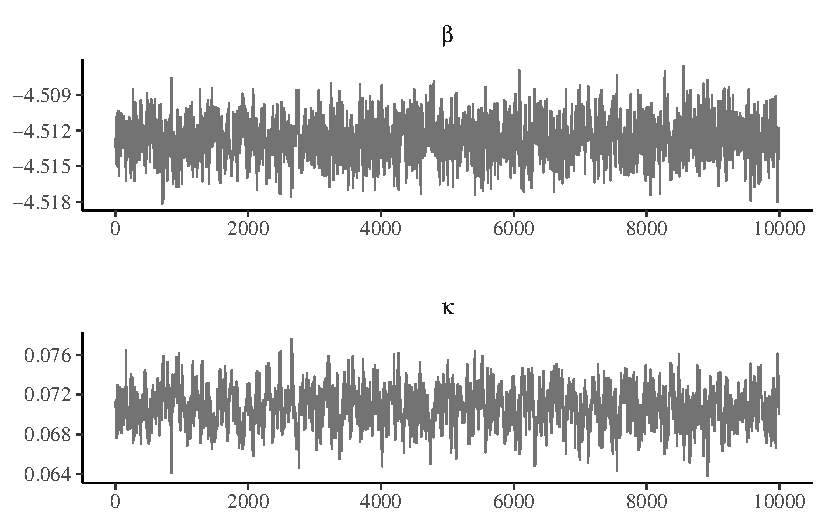
\includegraphics{mcmc_files/figure-pdf/fig-traceplot-1.pdf}

}

\caption{\label{fig-traceplot}Traceplots of Markov chain of log rate and
log odds rate for the Metropolis--Hastings sampler applied to the
Upworthy question data.}

\end{figure}

Figure~\ref{fig-scatterplot-upworthy-question} shows the posterior
samples, which are very nearly bivariate Gaussian. The parametrization
in terms of log odds ratio induces strong negative dependence, so if we
were to sample \(\kappa\), then \(\beta\), we would have much larger
inefficiency and slower exploration. Instead, the code used a bivariate
Gaussian random walk proposal whose covariance matrix was taken as a
multiple of the inverse of the negative hessian (equivalently, to the
observed information matrix of the log posterior), evaluated at of the
maximum a posteriori. This Gaussian approximation is called
\textbf{Laplace approximation}: it is advisable to reparametrize the
model so that the distribution is nearly symmetric, so that the
approximation is good. In this example, because of the large sample, the
Gaussian approximation implied by Bernstein--von Mises' theorem is
excellent.

\begin{figure}[ht!]

{\centering 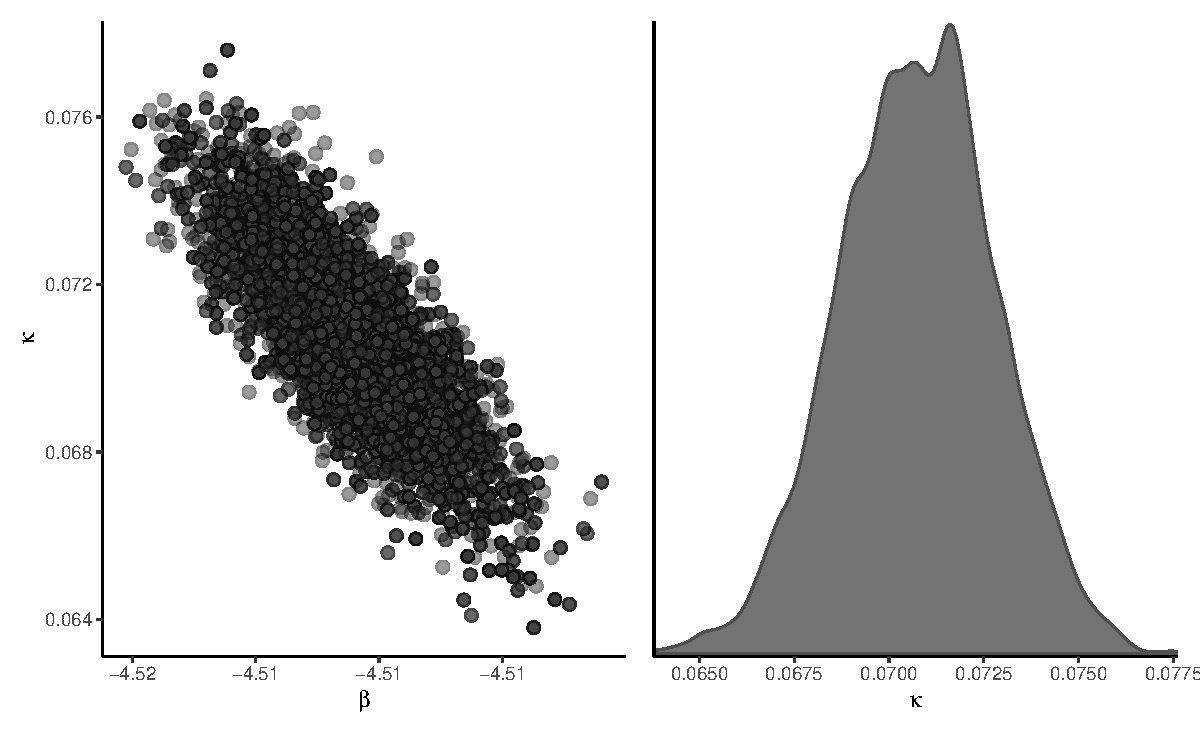
\includegraphics{mcmc_files/figure-pdf/fig-scatterplot-upworthy-question-1.pdf}

}

\caption{\label{fig-scatterplot-upworthy-question}Scatterplot of
posterior draws (left) and marginal density plot of log odds rate
(right).}

\end{figure}

\end{example}

The quality of the mixing of the chain (autocorrelation), depends on the
proposal variance, which can obtain by trial and error. Trace plots
Figure~\ref{fig-traceplot} show the values of the chain as a function of
iteration number. If our algorithm works well, we expect the proposals
to center around the posterior mode and resemble a fat hairy
caterpillar. If the variance is too small, the acceptance rate will
increase but most steps will be small. If the variance of the proposal
is too high, the acceptance rate will decrease (as many proposal moves
will have much lower posterior), so the chain will get stuck for long
periods of time. This is Goldilock's principle, as illustrated in
Figure~\ref{fig-goldilock-trace}.

\begin{figure}[ht!]

{\centering 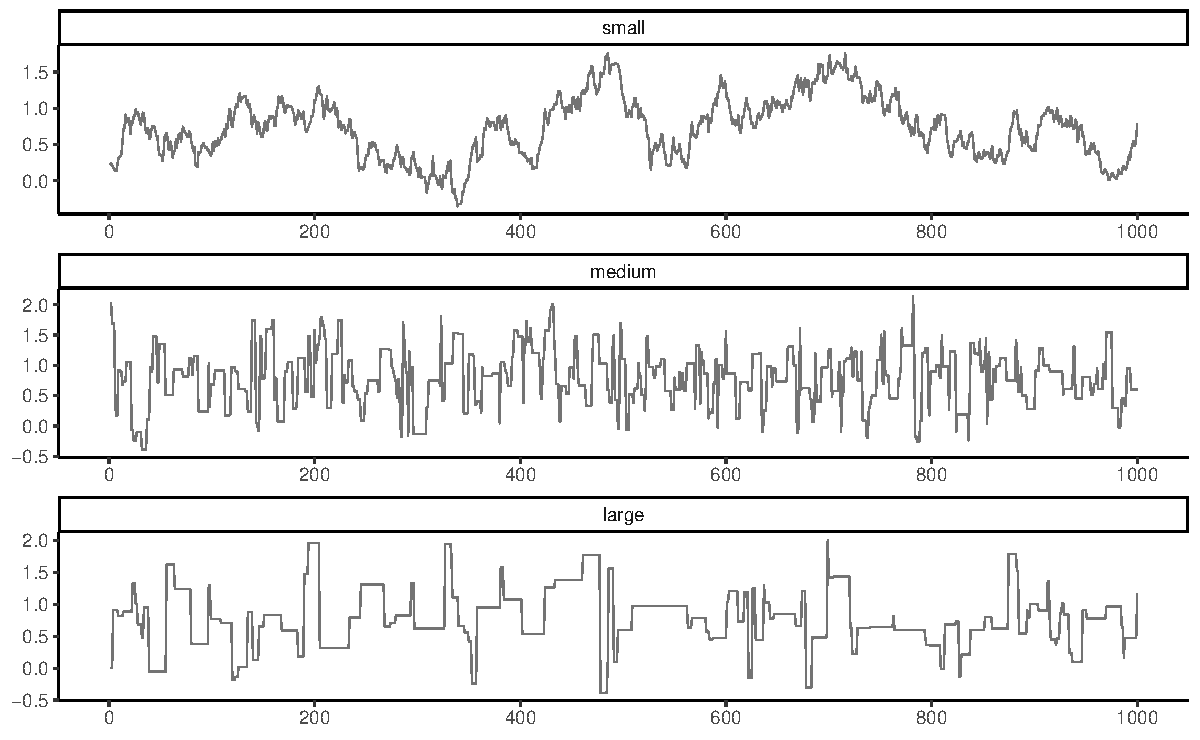
\includegraphics{mcmc_files/figure-pdf/fig-goldilock-trace-1.pdf}

}

\caption{\label{fig-goldilock-trace}Example of traceplot with proposal
variance that is too small (top), adequate (middle) and too large
(bottom).}

\end{figure}

One way to calibrate is to track the acceptance rate of the proposals:
for the three chains in Figure~\ref{fig-goldilock-trace}, these are
0.932, 0.33, 0.12. In one-dimensional toy problems with Gaussian
distributions, an acceptance rate of 0.44 is optimal, and this ratio
decreases to 0.234 when \(D \geq 2\) Sherlock
(\protect\hyperlink{ref-Sherlock:2013}{2013}). This need not generalize
to other settings and depends on the context. Optimal rate for
alternative algorithms, such as Metropolis-adjusted Langevin algorithm,
are typically higher.

We can tune the variance of the global proposal
(\protect\hyperlink{ref-Andrieu.Thoms:2008}{Andrieu and Thoms 2008}) to
improve the mixing of the chains at approximate stationarity. This is
done by increasing (decreasing) the variance if the historical
acceptance rate is too high (respectively low) during the burn in
period, and reinitializing after any change with an acceptance target of
\(0.44\). We stop adapting to ensure convergence to the posterior after
a suitable number of initial iterations. Adaptive MCMC methods use an
initial warm up period to find good proposals: we can consider a block
of length \(L\), compute the acceptance rate, multiply the variance by a
scaling factor and run the chain a little longer. We only keep samples
obtained after the adaptation phase.

We can also plot the autocorrelation of the entries of the chain as a
function of lags, a display known as correlogram in the time series
literature but colloquially referred to as autocorrelation function
(acf). The higher the autocorrelation, the more variance inflation one
has and the longer the number of steps before two draws are treated as
independent. Figure~\ref{fig-goldilock-correlogram} shows the effect of
the proposal variance on the correlation for the three chains.
Practitioners designing very inefficient Markov chain Monte Carlo
algorithms often thin their series: that is, they keep only every \(k\)
iteration. This is not recommended practice unless storage is an issue
and usually points towards inefficient sampling algorithms.

\begin{figure}[ht!]

{\centering 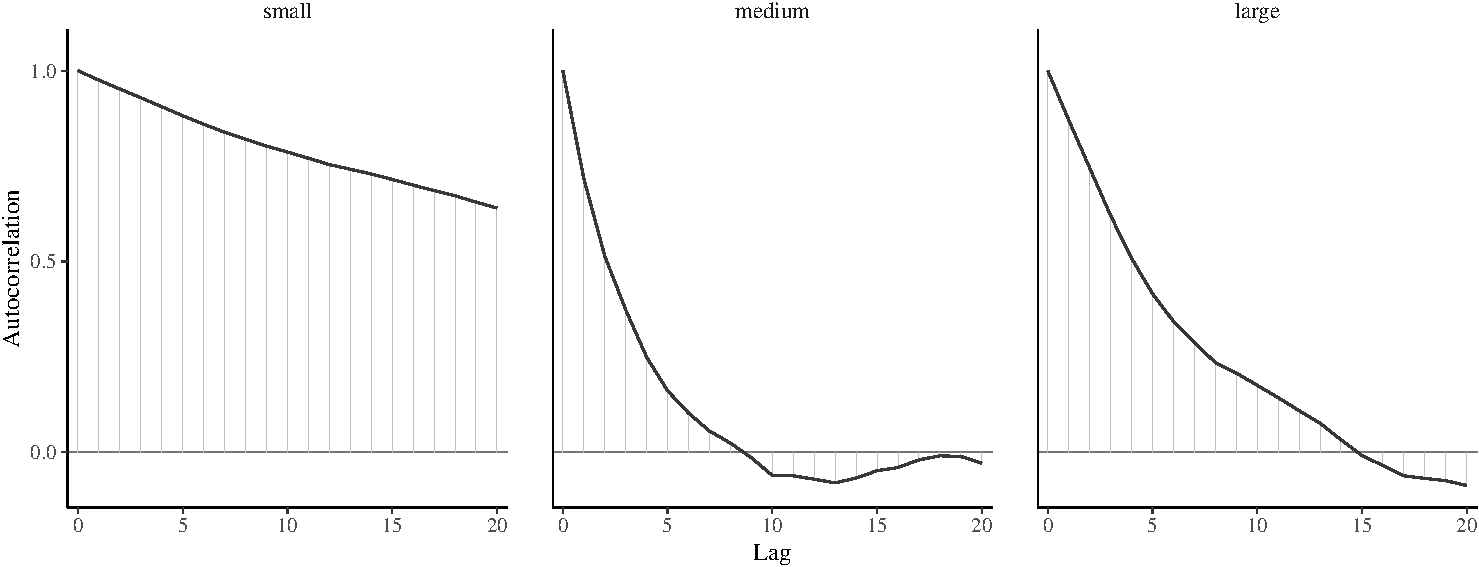
\includegraphics{mcmc_files/figure-pdf/fig-goldilock-correlogram-1.pdf}

}

\caption{\label{fig-goldilock-correlogram}Correlogram for the three
Markov chains.}

\end{figure}

\begin{remark}[Independence Metropolis--Hastings]

If the proposal density \(q(\cdot)\) does not depend on the current
state \(\boldsymbol{\theta}_{t-1}\), the algorithm is termed
\emph{independence}. To maximize acceptance, we could design a candidate
distribution whose mode is at the maximum a posteriori value. To
efficiently explore the state space, we need to place enough density in
all regions, for example by taking a heavy-tailed distributions, so that
we explore the full support. Such proposals can be however inefficient
and fail when the distribution of interest is multimodal. The
independence Metropolis--Hastings algorithm then resembles
accept-reject. If the ratio
\(p(\boldsymbol{\theta})/q(\boldsymbol{\theta})\) is bounded above by
\(C \geq 1\), then we can make comparisons with rejection sampling.
Lemma 7.9 of Robert and Casella
(\protect\hyperlink{ref-Robert.Casella:2004}{2004}) shows that the
probability of acceptance of a move for the Markov chain is at least
\(1/C\), which is larger than the accept-reject.

\end{remark}

In models with multiple parameter, we can use Metropolis--Hastings
algorithm to update every parameter in turn, fixing the value of the
others, rather than update them in block. The reason behind this
pragmatic choice is that, as for ordinary Monte Carlo sampling, the
acceptance rate goes down sharply with the dimension of the vector.
Updating parameters one at a time can lead to higher acceptance rates,
but slower exploration as a result of the correlation between
parameters.

If we can factorize the log posterior, then some updates may not depend
on all parameters: in a hierarchical model, hyperpriors parameter only
appear through priors, etc. This can reduce computational costs.

\begin{proposition}[Parameter
transformation]\protect\hypertarget{prp-parameter-transformation}{}\label{prp-parameter-transformation}

If a parameter is bounded in the interval \((a,b)\), where
\(-\infty \leq a < b \leq \infty\), we can consider a bijective
transformation \(\vartheta \equiv t(\theta): (a,b) \to \mathbb{R}\) with
differentiable inverse. The log density of the transformed variable,
assuming it exists, is \begin{align*}
f_\vartheta(\vartheta) = f_{\theta}\{t^{-1}(\vartheta)\} \left| \frac{\mathrm{d}}{\mathrm{d} \vartheta} t^{-1}(\vartheta)\right|
\end{align*} For example, we can use of the following transformations
for finite \(a, b\) in the software:

\begin{itemize}
\tightlist
\item
  if \(\theta \in (a, \infty)\) (lower bound only), then
  \(\vartheta = \log(\theta-a)\) and
  \(f_{\vartheta}(\vartheta)=f_{\theta}\{\exp(\vartheta) + a\}\cdot \exp(\vartheta)\)
\item
  if \(\theta \in (-\infty, b)\) (upper bound only), then
  \(\vartheta = \log(b-\theta)\) and
  \(f_{\vartheta}(\vartheta)=f_{\theta}\{b-\exp(\vartheta)\}\cdot \exp(\vartheta)\)
\item
  if \(\theta \in (a, b)\) (both lower and upper bound), then
  \(\vartheta = \mathrm{logit}\{(\theta-a)/(b-a)\}\) and \begin{align*}
  f_{\vartheta}(\vartheta)&=f_{\theta}\{a+(b-a) \mathrm{expit}(\vartheta)\} (b-a)\\&\quad \times \mathrm{expit}(\vartheta)\{1-\mathrm{expit}(\vartheta)\}
  \end{align*}
\end{itemize}

To guarantee that our proposals fall in the support of \(\theta\), we
can thus run a symmetric random walk proposal on the \emph{transformed
scale} by drawing \(\vartheta_{t}^{\star} \sim \vartheta_{t-1}+\tau Z\)
where \(Z\sim\mathsf{Norm}(0, 1)\). Due to the transformation, the
kernel ratio now contains the Jacobian.

\end{proposition}

\begin{proposition}[Truncated
proposals]\protect\hypertarget{prp-truncated-proposals}{}\label{prp-truncated-proposals}

As an alternative, if we are dealing with parameters that are restricted
in \([a,b]\), we can simulate using a random walk but with truncated
Gaussian steps, taking
\(\theta^{\star}_{t} \sim \mathsf{TruncNorm}(\vartheta_{t-1}, \tau^2, a, b).\)
The benefits of using the truncated proposal becomes more apparent when
we move to more advanced proposals whose mean and variance depends on
the gradient and or the hessian of the underlying unnormalized log
posterior, as the mean can be lower than \(a\) or larger than \(b\):
this would garantee zero acceptance with regular Gaussian random walk.
The \texttt{TruncatedNormal} package can be used to efficiently evaluate
such instances using results from Botev and L'Écuyer
(\protect\hyperlink{ref-LEcuyer.Botev:2017}{2017}) even when the
truncation bounds are far from the mode. the normalizing constant of the
truncated Gaussian in the denominator of the density is a function of
the location and scale parameters: if these depend on the current value
of \(\boldsymbol{\theta}_{t-1}\), as is the case for a random walk, we
need to keep these terms as part of the Metropolis ratio. The mean and
standard deviation of the truncated Gaussian are not equal to the
parameters \(\mu\) (which corresponds to the mode, provided
\(a < \mu < b\)) and \(\sigma\).

\end{proposition}

\begin{proposition}[Efficient
proposals]\protect\hypertarget{prp-mala}{}\label{prp-mala}

Rather than simply build a random walk, we can exploit the geometry of
the posterior using the gradient, via Metropolis-ajusted Langevin
algorithm (MALA), or using local quadratic approximations of the target.

Let \(p(\theta)\) denote the conditional (unnormalized) log posterior
for a scalar parameter \(\theta \in (a, b)\). We considering a Taylor
series expansion of \(p(\cdot)\) around the current parameter value
\(\theta_{t-1}\), \begin{align*}
 p(\theta) \approx p(\theta_{t-1}) + p'(\theta_{t-1})(\theta - \theta_{t-1}) + \frac{1}{2} p''(\theta_{t-1})(\theta - \theta_{t-1})^2
\end{align*} plus remainder, which suggests a Gaussian approximation
with mean
\(\mu_{t-1} = \theta_{t-1} - f'(\theta_{t-1})/f''(\theta_{t-1})\) and
precision \(\tau^{-2} = -f''(\theta_{t-1})\). We can use truncated
Gaussian distribution on \((a, b)\) with mean \(\mu\) and standard
deviation \(\tau\), denoted \(\mathsf{TruncNorm}(\mu, \tau, a, b)\) with
corresponding density function \(q(\cdot; \mu, \tau, a, b)\). The
Metropolis acceptance ratio for a proposal
\(\theta^{\star}_{t} \sim \mathsf{TruncNorm}(\mu_{t-1}, \tau_{t-1}, a, b)\)
is \begin{align*}
 \alpha = \frac{p(\theta^{\star}_{t})}{p(\theta_{t-1})} \frac{ q(\theta_{t-1} \mid \mu_{t}^{\star}, \tau_{t}^{\star}, a, b)}{q(\theta^{\star}_{t} \mid \mu_{t-1}, \tau_{t-1}, a, b)}
\end{align*} and we set \(\theta^{(t+1)} = \theta^{\star}_{t}\) with
probability \(\min\{1, r\}\) and \(\theta^{(t+1)} = \theta_{t-1}\)
otherwise. To evaluate the ratio of truncated Gaussian densities
\(q(\cdot; \mu, \tau, a, b)\), we need to compute the Taylor
approximation from the current parameter value, but also the reverse
move from the proposal \(\theta^{\star}_{t}\). Another option is to
modify the move dictated by the rescaled gradient by taking instead
\[\mu_{t-1} = \theta_{t-1} - \eta f'(\theta_{t-1})/f''(\theta_{t-1}).\]
The proposal includes an additional tuning parameter, \(\eta \leq 1\),
whose role is to prevent oscillations of the quadratic approximation, as
in a Newton--Raphson algorithm. Relative to a random walk
Metropolis--Hastings, the proposal automatically adjusts to the local
geometry of the target, which guarantees a higher acceptance rate and
lower autocorrelation for the Markov chain despite the higher evaluation
costs. The proposal requires that both \(f''(\theta_{t-1})\) and
\(f''(\theta^{\star}_{t})\) be negative since the variance is
\(-1/f''(\theta)\): this shouldn't be problematic in the vicinity of the
mode. Otherwise, one could use a global scaling derived from the hessian
at the mode.

The simpler Metropolis-adjusted Langevin algorithm is equivalent to
using a Gaussian random walk where the proposal has mean
\(\boldsymbol{\theta}_{t-1} + \mathbf{A}\eta \nabla \ell(\boldsymbol{\theta}_{t-1})\)
and variance \(\tau^2\mathbf{A}\), for some mass matrix
\(\boldsymbol{A}\) and a damping factor \(\eta\). Taking \(\mathbf{A}\)
as the identity matrix, which assumes the parameters are isotropic (same
variance, uncorrelated) is the default choice although seldom far from
optimal.

For MALA to work well, we need both to start near stationarity, to
ensure that the gradient is relatively small and to prevent
oscillations. One can dampen the size of the step initially if needed to
avoid overshooting. The proposal variance, the other tuning parameter,
is critical to the success of the algorithm. The usual target for the
variance is one that gives an acceptance rate of roughly 0.574. These
more efficient methods require additional calculations of the gradient
and Hessian, either numerically or analytically. Depending on the
situation and the computational costs of such calculations, the
additional overhead may not be worth it.

\end{proposition}

\begin{example}[]\protect\hypertarget{exm-normal-question-upworthy}{}\label{exm-normal-question-upworthy}

We revisit the Upworthy data, this time modelling each individual
headline as a separate observation. We view \(n=\)\texttt{nimpression}
as the sample size of a binomial distribution and \texttt{nclick} as the
number of successes. Since the number of trials is large, the sample
average \texttt{nclick}/\texttt{nimpression}, denoted \(y\) in the
sequel, is approximately Gaussian. We assume that each story has a
similar population rate and capture the heterogeneity inherent to each
news story by treating each mean as a sample. The variance of the sample
average or click rate is proportional to \(n^{-1}\), where \(n\) is the
number of impressions. To allow for underdispersion or overdispersion,
we thus consider a Gaussian likelihood
\(Y_i \sim \mathsf{Norm}(\mu, \sigma^2/n_i)\). We perform Bayesian
inference for \(\mu, \sigma\) after assigning a truncated Gaussian prior
for \(\mu \sim \mathsf{TruncNorm}(0.01, 0.1^2)\) over \([0,1]\) and an
penalized complexity prior for \(\sigma \sim \mathsf{Exp}(0.7)\).

\begin{Shaded}
\begin{Highlighting}[]
\FunctionTok{data}\NormalTok{(upworthy\_question, }\AttributeTok{package =} \StringTok{"hecbayes"}\NormalTok{)}
\CommentTok{\# Select data for a single question}
\NormalTok{qdata }\OtherTok{\textless{}{-}}\NormalTok{ upworthy\_question }\SpecialCharTok{|\textgreater{}}
\NormalTok{  dplyr}\SpecialCharTok{::}\FunctionTok{filter}\NormalTok{(question }\SpecialCharTok{==} \StringTok{"yes"}\NormalTok{) }\SpecialCharTok{|\textgreater{}}
\NormalTok{  dplyr}\SpecialCharTok{::}\FunctionTok{mutate}\NormalTok{(}\AttributeTok{y =}\NormalTok{ clicks}\SpecialCharTok{/}\NormalTok{impressions,}
                \AttributeTok{no =}\NormalTok{ impressions)}
\CommentTok{\# Create functions with the same signature (...) for the algorithm}
\NormalTok{logpost }\OtherTok{\textless{}{-}} \ControlFlowTok{function}\NormalTok{(par, data, ...)\{}
\NormalTok{  mu }\OtherTok{\textless{}{-}}\NormalTok{ par[}\DecValTok{1}\NormalTok{]; sigma }\OtherTok{\textless{}{-}}\NormalTok{ par[}\DecValTok{2}\NormalTok{]}
\NormalTok{  no }\OtherTok{\textless{}{-}}\NormalTok{ data}\SpecialCharTok{$}\NormalTok{no}
\NormalTok{  y }\OtherTok{\textless{}{-}}\NormalTok{ data}\SpecialCharTok{$}\NormalTok{y}
  \ControlFlowTok{if}\NormalTok{(}\FunctionTok{isTRUE}\NormalTok{(}\FunctionTok{any}\NormalTok{(sigma }\SpecialCharTok{\textless{}=} \DecValTok{0}\NormalTok{, mu }\SpecialCharTok{\textless{}} \DecValTok{0}\NormalTok{, mu }\SpecialCharTok{\textgreater{}} \DecValTok{1}\NormalTok{)))\{}
    \FunctionTok{return}\NormalTok{(}\SpecialCharTok{{-}}\ConstantTok{Inf}\NormalTok{)}
\NormalTok{  \}}
  \FunctionTok{dnorm}\NormalTok{(}\AttributeTok{x =}\NormalTok{ mu, }\AttributeTok{mean =} \FloatTok{0.01}\NormalTok{, }\AttributeTok{sd =} \FloatTok{0.1}\NormalTok{, }\AttributeTok{log =} \ConstantTok{TRUE}\NormalTok{) }\SpecialCharTok{+}
  \FunctionTok{dexp}\NormalTok{(sigma, }\AttributeTok{rate =} \FloatTok{0.7}\NormalTok{, }\AttributeTok{log =} \ConstantTok{TRUE}\NormalTok{) }\SpecialCharTok{+} 
  \FunctionTok{sum}\NormalTok{(}\FunctionTok{dnorm}\NormalTok{(}\AttributeTok{x =}\NormalTok{ y, }\AttributeTok{mean =}\NormalTok{ mu, }\AttributeTok{sd =}\NormalTok{ sigma}\SpecialCharTok{/}\FunctionTok{sqrt}\NormalTok{(no), }\AttributeTok{log =} \ConstantTok{TRUE}\NormalTok{))}
\NormalTok{\}}

\NormalTok{logpost\_grad }\OtherTok{\textless{}{-}} \ControlFlowTok{function}\NormalTok{(par, data, ...)\{}
\NormalTok{   no }\OtherTok{\textless{}{-}}\NormalTok{ data}\SpecialCharTok{$}\NormalTok{no}
\NormalTok{  y }\OtherTok{\textless{}{-}}\NormalTok{ data}\SpecialCharTok{$}\NormalTok{y}
\NormalTok{  mu }\OtherTok{\textless{}{-}}\NormalTok{ par[}\DecValTok{1}\NormalTok{]; sigma }\OtherTok{\textless{}{-}}\NormalTok{ par[}\DecValTok{2}\NormalTok{]}
  \FunctionTok{c}\NormalTok{(}\FunctionTok{sum}\NormalTok{(no}\SpecialCharTok{*}\NormalTok{(y}\SpecialCharTok{{-}}\NormalTok{mu))}\SpecialCharTok{/}\NormalTok{sigma}\SpecialCharTok{\^{}}\DecValTok{2} \SpecialCharTok{{-}}\NormalTok{(mu }\SpecialCharTok{{-}} \FloatTok{0.01}\NormalTok{)}\SpecialCharTok{/}\FloatTok{0.01}\NormalTok{,}
    \SpecialCharTok{{-}}\FunctionTok{length}\NormalTok{(y)}\SpecialCharTok{/}\NormalTok{sigma }\SpecialCharTok{+} \FunctionTok{sum}\NormalTok{(no}\SpecialCharTok{*}\NormalTok{(y}\SpecialCharTok{{-}}\NormalTok{mu)}\SpecialCharTok{\^{}}\DecValTok{2}\NormalTok{)}\SpecialCharTok{/}\NormalTok{sigma}\SpecialCharTok{\^{}}\DecValTok{3} \SpecialCharTok{{-}}\FloatTok{0.7}
\NormalTok{  )}
\NormalTok{\}}

\CommentTok{\# Starting values {-} MAP}
\NormalTok{map }\OtherTok{\textless{}{-}} \FunctionTok{optim}\NormalTok{(}
  \AttributeTok{par =} \FunctionTok{c}\NormalTok{(}\FunctionTok{mean}\NormalTok{(qdata}\SpecialCharTok{$}\NormalTok{y), }\FloatTok{0.5}\NormalTok{),}
  \AttributeTok{fn =} \ControlFlowTok{function}\NormalTok{(x)\{}\SpecialCharTok{{-}}\FunctionTok{logpost}\NormalTok{(x, }\AttributeTok{data =}\NormalTok{ qdata)\},}
  \AttributeTok{gr =} \ControlFlowTok{function}\NormalTok{(x)\{}\SpecialCharTok{{-}}\FunctionTok{logpost\_grad}\NormalTok{(x, }\AttributeTok{data =}\NormalTok{ qdata)\},  }
  \AttributeTok{hessian =} \ConstantTok{TRUE}\NormalTok{,}
  \AttributeTok{method =} \StringTok{"BFGS"}\NormalTok{)}
\CommentTok{\# Set initial parameter values}
\NormalTok{curr }\OtherTok{\textless{}{-}}\NormalTok{ map}\SpecialCharTok{$}\NormalTok{par }
\CommentTok{\# Check convergence }
\FunctionTok{logpost\_grad}\NormalTok{(curr, }\AttributeTok{data =}\NormalTok{ qdata)}
\end{Highlighting}
\end{Shaded}

\begin{verbatim}
[1] 7.650733e-03 5.575424e-05
\end{verbatim}

\begin{Shaded}
\begin{Highlighting}[]
\CommentTok{\# Compute a mass matrix}
\NormalTok{Amat }\OtherTok{\textless{}{-}} \FunctionTok{solve}\NormalTok{(map}\SpecialCharTok{$}\NormalTok{hessian)}
\CommentTok{\# Cholesky root {-} for random number generation}
\NormalTok{cholA }\OtherTok{\textless{}{-}} \FunctionTok{chol}\NormalTok{(Amat)}



\CommentTok{\# Create containers for MCMC}
\NormalTok{B }\OtherTok{\textless{}{-}} \FloatTok{1e4}\NormalTok{L }\CommentTok{\# number of iterations}
\NormalTok{warmup }\OtherTok{\textless{}{-}} \FloatTok{1e3}\NormalTok{L }\CommentTok{\# adaptation period}
\NormalTok{prop\_sd }\OtherTok{\textless{}{-}} \FunctionTok{rep}\NormalTok{(}\DecValTok{1}\NormalTok{, }\DecValTok{2}\NormalTok{)}
\NormalTok{npar }\OtherTok{\textless{}{-}}\NormalTok{ 2L}
\NormalTok{chains }\OtherTok{\textless{}{-}} \FunctionTok{matrix}\NormalTok{(}\AttributeTok{nrow =}\NormalTok{ B, }\AttributeTok{ncol =}\NormalTok{ npar)}
\NormalTok{damping }\OtherTok{\textless{}{-}} \FloatTok{0.8}
\NormalTok{acceptance }\OtherTok{\textless{}{-}}\NormalTok{ attempts }\OtherTok{\textless{}{-}} \DecValTok{0} 
\FunctionTok{colnames}\NormalTok{(chains) }\OtherTok{\textless{}{-}} \FunctionTok{names}\NormalTok{(curr) }\OtherTok{\textless{}{-}} \FunctionTok{c}\NormalTok{(}\StringTok{"mu"}\NormalTok{,}\StringTok{"sigma"}\NormalTok{)}
\NormalTok{prop\_var }\OtherTok{\textless{}{-}} \FunctionTok{diag}\NormalTok{(prop\_sd) }\SpecialCharTok{\%*\%}\NormalTok{ Amat }\SpecialCharTok{\%*\%} \FunctionTok{diag}\NormalTok{(prop\_sd)}
\ControlFlowTok{for}\NormalTok{(i }\ControlFlowTok{in} \FunctionTok{seq\_len}\NormalTok{(B }\SpecialCharTok{+}\NormalTok{ warmup))\{}
\NormalTok{  ind }\OtherTok{\textless{}{-}} \FunctionTok{pmax}\NormalTok{(}\DecValTok{1}\NormalTok{, i }\SpecialCharTok{{-}}\NormalTok{ warmup)}
  \CommentTok{\# Compute the proposal mean for the Newton step}
\NormalTok{  prop\_mean }\OtherTok{\textless{}{-}} \FunctionTok{c}\NormalTok{(curr }\SpecialCharTok{+}\NormalTok{ damping }\SpecialCharTok{*} 
\NormalTok{     Amat }\SpecialCharTok{\%*\%} \FunctionTok{logpost\_grad}\NormalTok{(curr, }\AttributeTok{data =}\NormalTok{ qdata))}
  \CommentTok{\# prop \textless{}{-} prop\_sd * c(rnorm(npar) \%*\% cholA) + prop\_mean}
\NormalTok{  prop }\OtherTok{\textless{}{-}} \FunctionTok{c}\NormalTok{(mvtnorm}\SpecialCharTok{::}\FunctionTok{rmvnorm}\NormalTok{(}
    \AttributeTok{n =} \DecValTok{1}\NormalTok{,}
    \AttributeTok{mean =}\NormalTok{ prop\_mean, }
    \AttributeTok{sigma =}\NormalTok{ prop\_var))}
  \CommentTok{\# Compute the reverse step}
\NormalTok{  curr\_mean }\OtherTok{\textless{}{-}} \FunctionTok{c}\NormalTok{(prop }\SpecialCharTok{+}\NormalTok{ damping }\SpecialCharTok{*} 
\NormalTok{     Amat }\SpecialCharTok{\%*\%} \FunctionTok{logpost\_grad}\NormalTok{(prop, }\AttributeTok{data =}\NormalTok{ qdata))}
  \CommentTok{\# log of ratio of bivariate Gaussian densities}
\NormalTok{  logmh }\OtherTok{\textless{}{-}}\NormalTok{ mvtnorm}\SpecialCharTok{::}\FunctionTok{dmvnorm}\NormalTok{(}
    \AttributeTok{x =}\NormalTok{ curr, }\AttributeTok{mean =}\NormalTok{ prop\_mean, }
    \AttributeTok{sigma =}\NormalTok{ prop\_var, }
    \AttributeTok{log =} \ConstantTok{TRUE}\NormalTok{) }\SpecialCharTok{{-}} 
\NormalTok{    mvtnorm}\SpecialCharTok{::}\FunctionTok{dmvnorm}\NormalTok{(}
      \AttributeTok{x =}\NormalTok{ prop, }
      \AttributeTok{mean =}\NormalTok{ curr\_mean, }
      \AttributeTok{sigma =}\NormalTok{ prop\_var, }
      \AttributeTok{log =} \ConstantTok{TRUE}\NormalTok{) }\SpecialCharTok{+} 
  \FunctionTok{logpost}\NormalTok{(prop, }\AttributeTok{data =}\NormalTok{ qdata) }\SpecialCharTok{{-}} 
    \FunctionTok{logpost}\NormalTok{(curr, }\AttributeTok{data =}\NormalTok{ qdata)}
  \ControlFlowTok{if}\NormalTok{(logmh }\SpecialCharTok{\textgreater{}} \FunctionTok{log}\NormalTok{(}\FunctionTok{runif}\NormalTok{(}\DecValTok{1}\NormalTok{)))\{}
\NormalTok{    curr }\OtherTok{\textless{}{-}}\NormalTok{ prop}
\NormalTok{    acceptance }\OtherTok{\textless{}{-}}\NormalTok{ acceptance }\SpecialCharTok{+}\NormalTok{ 1L}
\NormalTok{  \}}
\NormalTok{  attempts }\OtherTok{\textless{}{-}}\NormalTok{ attempts }\SpecialCharTok{+}\NormalTok{ 1L}
  \CommentTok{\# Save current value}
\NormalTok{  chains[ind,] }\OtherTok{\textless{}{-}}\NormalTok{ curr}
  \ControlFlowTok{if}\NormalTok{(i }\SpecialCharTok{\%\%} \DecValTok{100} \SpecialCharTok{\&}\NormalTok{ i }\SpecialCharTok{\textless{}}\NormalTok{ warmup)\{}
\NormalTok{    out }\OtherTok{\textless{}{-}}\NormalTok{ hecbayes}\SpecialCharTok{::}\FunctionTok{adaptive}\NormalTok{(}
      \AttributeTok{attempts =}\NormalTok{ attempts, }
      \AttributeTok{acceptance =}\NormalTok{ acceptance, }
      \AttributeTok{sd.p =}\NormalTok{ prop\_sd,}
      \AttributeTok{target =} \FloatTok{0.574}\NormalTok{)}
\NormalTok{    prop\_sd }\OtherTok{\textless{}{-}}\NormalTok{ out}\SpecialCharTok{$}\NormalTok{sd}
\NormalTok{    acceptance }\OtherTok{\textless{}{-}}\NormalTok{ out}\SpecialCharTok{$}\NormalTok{acc}
\NormalTok{    attempts }\OtherTok{\textless{}{-}}\NormalTok{ out}\SpecialCharTok{$}\NormalTok{att}
\NormalTok{    prop\_var }\OtherTok{\textless{}{-}} \FunctionTok{diag}\NormalTok{(prop\_sd) }\SpecialCharTok{\%*\%}\NormalTok{ Amat }\SpecialCharTok{\%*\%} \FunctionTok{diag}\NormalTok{(prop\_sd)}
\NormalTok{  \}}
\NormalTok{\}}
\end{Highlighting}
\end{Shaded}

MALA requires critically a good mass matrix, especially if the gradient
is very large at the starting values (often the case when the starting
value is far from the mode). Given the precision of the original
observations, we did not need to modify anything to deal with the
parameter constraints \(0 \leq \mu \leq 1\) and \(\sigma>0\), outside of
encoding them in the log posterior function.

The posterior mean for the standard deviation is 0.64, which suggests
overdispersion.

\end{example}

\hypertarget{gibbs-sampling}{%
\section{Gibbs sampling}\label{gibbs-sampling}}

The Gibbs sampling algorithm builds a Markov chain by iterating through
a sequence of conditional distributions. Consider a model with
\(\boldsymbol{\theta} \in \boldsymbol{\Theta} \subseteq \mathbb{R}^p\).
We consider a single (or \(m \leq p\) blocks of parameters), say
\(\boldsymbol{\theta}^{[j]}\), such that, conditional on the remaining
components of the parameter vector \(\boldsymbol{\theta}^{-[j]}\), the
conditional posterior
\(p(\boldsymbol{\theta}^{[j]} \mid \boldsymbol{\theta}^{-[j]}, \boldsymbol{y})\)
is from a known distribution from which we can simulate draws

At iteration \(t\), we can update each block in turn: note that the
\(k\)th block uses the partially updated state \begin{align*}
\boldsymbol{\theta}^{-[k]\star} = (\boldsymbol{\theta}_{t}^{[1]}, \ldots, \boldsymbol{\theta}_{t}^{[k-1]},\boldsymbol{\theta}_{t-1}^{[k+1]}, \boldsymbol{\theta}_{t-1}^{[m]})
\end{align*} which corresponds to the current value of the parameter
vector after the updates. To check the validity of the Gibbs sampler,
see the methods proposed in Geweke
(\protect\hyperlink{ref-Geweke:2004}{2004}).

The Gibbs sampling can be viewed as a special case of
Metropolis--Hastings where the proposal distribution \(q\) is
\(p(\boldsymbol{\theta}^{[j]} \mid \boldsymbol{\theta}^{-[j]\star}, \boldsymbol{y})\).
The particularity is that all proposals get accepted because the log
posterior of the partial update, equals the proposal distribution, so
\begin{align*}
R = \frac{p(\boldsymbol{\theta}_t^{[j]\star} \mid \boldsymbol{\theta}^{-[j]\star}, \boldsymbol{y})}{p(\boldsymbol{\theta}_{t-1}^{[j]\star} \mid \boldsymbol{\theta}^{-[j]\star}, \boldsymbol{y})}\frac{p(\boldsymbol{\theta}_{t-1}^{[j]\star} \mid \boldsymbol{\theta}^{-[j]\star}, \boldsymbol{y})}{p(\boldsymbol{\theta}_t^{[j]\star} \mid \boldsymbol{\theta}^{-[j]\star}, \boldsymbol{y})}=1.
\end{align*} Regardless of the order (systematic scan or random scan),
the procedure remains valid. The Gibbs sampling is thus an automatic
algorithm: we only need to derive the conditional posterior
distributions of the parameters and run the sampler, and there are no
tuning parameter involved. If the parameters are strongly correlated,
the changes for each parameter will be incremental and this will lead to
slow mixing and large autocorrelation, even if the values drawn are all
different. Figure~\ref{fig-Gibbs-steps} shows 25 steps from a Gibbs
algorithm for a bivariate target.

\begin{figure}[ht!]

{\centering 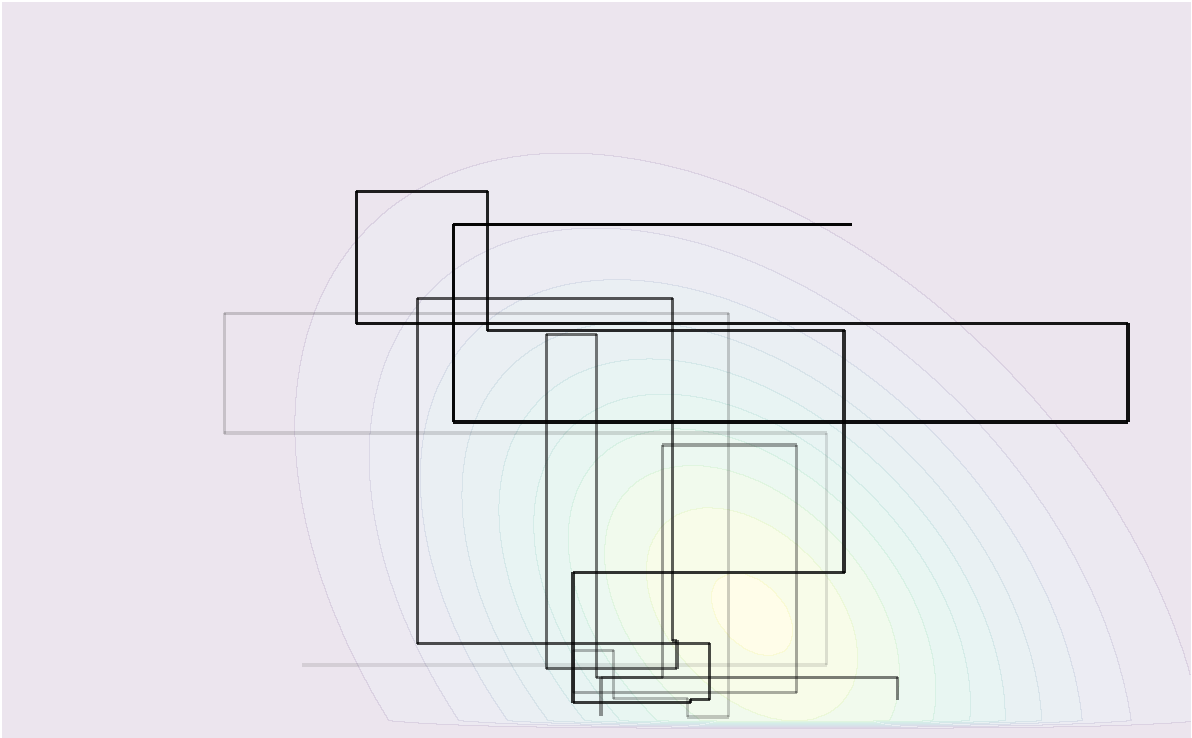
\includegraphics{mcmc_files/figure-pdf/fig-Gibbs-steps-1.pdf}

}

\caption{\label{fig-Gibbs-steps}Sampling trajectory for a bivariate
target using Gibbs sampling.}

\end{figure}

As a toy illustration, we use Gibbs sampling to simulate data from a
\(d\)-dimensional multivariate Gaussian target with mean
\(\boldsymbol{\mu}\) and equicorrelation covariance matrix
\(\mathbf{\Sigma} = (1-\rho)\mathbf{I}_d + \rho\boldsymbol{1}_{d}\boldsymbol{1}^\top_d\)
with inverse
\[\mathbf{Q} = \boldsymbol{\Sigma}^{-1}=(1-\rho)^{-1}\left\{\mathbf{I}_d - \rho \mathbf{1}_d\mathbf{1}_d/(1+(d-1)\rho)\right\},\]
for known correlation coefficient \(\rho\). While we can easily sample
independent observations, the exercise is insightful to see how well the
methods works as the dimension increases, and when the correlation
between pairs becomes stronger.

Consider
\(\boldsymbol{Y} \sim \mathsf{Norm}_d(\boldsymbol{\mu}, \boldsymbol{\Sigma})\)
and a partition \((\boldsymbol{Y}_1^\top, \boldsymbol{Y}_2^\top)^\top\):
the conditional distribution of the \(k\) subvector \(\boldsymbol{Y}_1\)
given the \(d-k\) other components \(\boldsymbol{Y}_2\) is, in terms of
either the covariance (first line) or the precision (second line),
Gaussian where \begin{align*}
\boldsymbol{Y}_1 \mid \boldsymbol{Y}_2=\boldsymbol{y}_2 &\sim \mathsf{Norm}_{k}\left\{ \boldsymbol{\mu}_1 + \boldsymbol{\Sigma}_{12} \boldsymbol{\Sigma}_{22}^{-1}(\boldsymbol{y}_2 - \boldsymbol{\mu}_2), \boldsymbol{\Sigma}_{11} - \boldsymbol{\Sigma}_{12}\boldsymbol{\Sigma}_{22}^{-1}\boldsymbol{\Sigma}_{21}\right\}
\\&\sim \mathsf{Norm}_{k}\left\{ \boldsymbol{\mu}_1 -\mathbf{Q}_{11}^{-1}\mathbf{Q}_{12}(\boldsymbol{y}_2 - \boldsymbol{\mu}_2), \mathbf{Q}_{11}^{-1}\right\}.
\end{align*}

\begin{Shaded}
\begin{Highlighting}[]
\CommentTok{\# Create a 20 dimensional equicorrelation}
\NormalTok{d }\OtherTok{\textless{}{-}} \DecValTok{20}
\NormalTok{Q }\OtherTok{\textless{}{-}}\NormalTok{ hecbayes}\SpecialCharTok{::}\FunctionTok{equicorrelation}\NormalTok{(}\AttributeTok{d =}\NormalTok{ d, }\AttributeTok{rho =} \FloatTok{0.9}\NormalTok{, }\AttributeTok{precision =} \ConstantTok{TRUE}\NormalTok{)}
\NormalTok{B }\OtherTok{\textless{}{-}} \FloatTok{1e4}
\NormalTok{chains }\OtherTok{\textless{}{-}} \FunctionTok{matrix}\NormalTok{(}\DecValTok{0}\NormalTok{, }\AttributeTok{nrow =}\NormalTok{ B, }\AttributeTok{ncol =}\NormalTok{ d)}
\NormalTok{mu }\OtherTok{\textless{}{-}} \FunctionTok{rep}\NormalTok{(}\DecValTok{2}\NormalTok{, d)}
\CommentTok{\# Start far from mode}
\NormalTok{curr }\OtherTok{\textless{}{-}} \FunctionTok{rep}\NormalTok{(}\SpecialCharTok{{-}}\DecValTok{3}\NormalTok{, d)}
\ControlFlowTok{for}\NormalTok{(i }\ControlFlowTok{in} \FunctionTok{seq\_len}\NormalTok{(B))\{}
  \CommentTok{\# Random scan, updating one variable at a time}
  \ControlFlowTok{for}\NormalTok{(j }\ControlFlowTok{in} \FunctionTok{sample}\NormalTok{(}\DecValTok{1}\SpecialCharTok{:}\NormalTok{d, }\AttributeTok{size =}\NormalTok{ d))\{}
    \CommentTok{\# sample from conditional Gaussian given curr}
\NormalTok{    curr[j] }\OtherTok{\textless{}{-}}\NormalTok{ hecbayes}\SpecialCharTok{::}\FunctionTok{rcondmvnorm}\NormalTok{(}
      \AttributeTok{n =} \DecValTok{1}\NormalTok{, }
      \AttributeTok{value =}\NormalTok{ curr, }
      \AttributeTok{ind =}\NormalTok{ j, }
      \AttributeTok{mean =}\NormalTok{ mu, }
      \AttributeTok{precision =}\NormalTok{ Q)}
\NormalTok{  \}}
\NormalTok{  chains[i,] }\OtherTok{\textless{}{-}}\NormalTok{ curr }\CommentTok{\# save values after full round of update}
\NormalTok{\}}
\end{Highlighting}
\end{Shaded}

As the dimension of the parameter space increases, and as the
correlation between components becomes larger, the efficiency of the
Gibbs sampler degrades: Figure~\ref{fig-gibbs-normal} shows the first
component for updating one-parameter at a time for a multivariate
Gaussian target in dimensions \(d=20\) and \(d=3\), started at four
deviation away from the mode. The chain makes smaller steps when there
is strong correlation, resulting in an inefficient sampler.

\begin{figure}[ht!]

{\centering 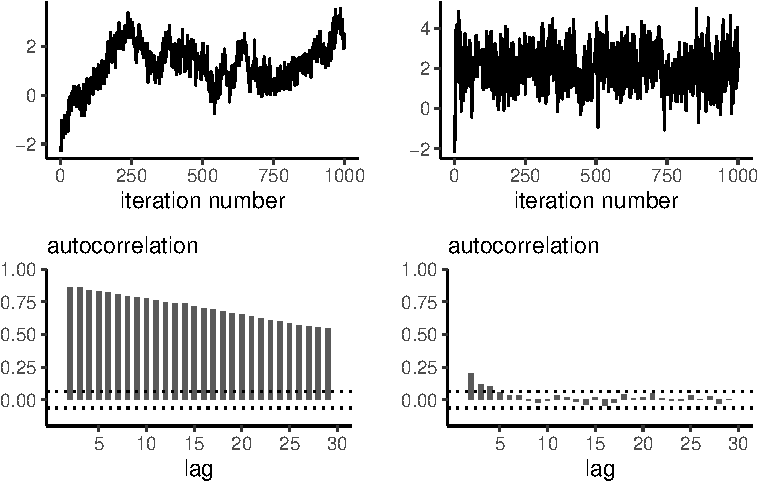
\includegraphics{mcmc_files/figure-pdf/fig-gibbs-normal-1.pdf}

}

\caption{\label{fig-gibbs-normal}Trace plots (top) and correlograms
(bottom) for the first component of a Gibbs sampler with \(d=20\)
equicorrelated Gaussian variates with correlation \(\rho=0.9\) (left)
and \(d=3\) with equicorrelation \(\rho=0.5\) (right).}

\end{figure}

The main bottleneck in Gibbs sampling is determining all of the relevant
conditional distributions, which often relies on setting conditionally
conjugate priors. In large models with multiple layers, full
conditionals may only depend on a handful of parameters.

\begin{example}[]\protect\hypertarget{exm-gaussian-gamma}{}\label{exm-gaussian-gamma}

Consider a Gaussian model \(Y_i \sim \mathsf{Norm}(\mu, \tau)\)
(\(i=1, \ldots, n\)) are independent, and where we assign priors
\(\mu \sim \mathsf{Norm}(\nu, \omega)\) and
\(\sigma \sim \mathsf{InvGamma}(\alpha, \beta)\).

The joint posterior is not available in closed form, but the independent
priors for the mean and variance of the observations are conditionally
conjugate, since the joint posterior \begin{align*}
p(\mu, \tau \mid \boldsymbol{y}) \propto& \tau^{-n/2}\exp\left\{-\frac{1}{2\tau}\left(\sum_{i=1}^n y_i^2 - 2\mu \sum_{i=1}^n y_i+n\mu^2 \right)\right\}\\& \times \exp\left\{-\frac{(\mu-\nu)^2}{2\omega}\right\} \times \tau^{-\alpha-1}\exp(-\beta/\tau)
\end{align*} gives us \begin{align*}
p(\mu \mid \tau, \boldsymbol{y}) &\propto \exp\left\{-\frac{1}{2} \left( \frac{\mu^2-2\mu\overline{y}}{\tau/n} + \frac{\mu^2-2\nu \mu}{\omega}\right)\right\}\\
p(\tau \mid \mu, \boldsymbol{y}) & \propto \tau^{-n/2-\alpha-1}\exp\left[-\left\{\frac{\sum_{i=1}^n (y_i-\mu)^2}{2} + \beta \right\}/\tau\right]
\end{align*} so we can simulate in turn \begin{align*}
\mu_t \mid \tau_{t-1}, \boldsymbol{y} &\sim \mathsf{Norm}\left(\frac{n\overline{y}\omega+\tau \nu}{\omega\tau}, \frac{\omega \tau}{\tau + \omega/n}\right)\\
\tau_t \mid \mu_t, \boldsymbol{y} &\sim \mathsf{InvGamma}\left\{\frac{n}{2}+\alpha, \frac{\sum_{i=1}^n (y_i-\mu)^2}{2} + \beta\right\}.
\end{align*}

\end{example}

\begin{remark}[Gibbs sampler and proper posterior]

Gibbs sampling cannot be used to determine if the posterior is improper.
If the posterior is not well defined, the Markov chains may seem to
stabilize even though there is no proper target.

\end{remark}

\begin{proposition}[Conjugate priors in the Bayesian linear
model]\protect\hypertarget{prp-conjugate-bayesian-linmod}{}\label{prp-conjugate-bayesian-linmod}

Consider a linear regression model with observation-specific mean
\(\mu_i = \mathbf{x}_i\boldsymbol{\beta}\) \((i=1,\ldots, n)\) with
\(\mathbf{x}_i\) the \(i\)th row of the \(n \times p\) model matrix
\(\mathbf{X}\).

Concatenating records,
\(\boldsymbol{Y} \sim \mathsf{No}_n(\mathbf{X}\boldsymbol{\beta}, \sigma^2 \mathbf{Q}_y^{-1})\),
for a known precision matrix \(\mathbf{Q}_y\), typically
\(\mathbf{I}_n\). To construct a conjugate joint prior for
\(p(\boldsymbol{\beta}, \sigma^2)\), we consider the sequential
formulation \begin{align*}
\boldsymbol{\beta} \mid \sigma^2 \sim \mathsf{Norm}_p(\boldsymbol{\nu}_\beta, \sigma^2 \mathbf{Q}^{-1}_\beta), \qquad \sigma^2 \sim \mathsf{InvGamma}(\alpha,\beta)
\end{align*} where \(\mathsf{InvGamma}\) denotes the inverse gamma
distribution\footnote{This simply means that the precision
  \(\sigma^{-2}\), the reciprocal of the variance, has a gamma
  distribution with shape \(\alpha\) and rate \(\beta\).}

The joint posterior is Gaussian-inverse gamma and can be factorized
\begin{align*}
p(\boldsymbol{\beta}, \sigma^2 \mid y) = p(\sigma^2 \mid y) p(\boldsymbol{\beta} \mid \sigma^2, y)
\end{align*} where
\(p(\sigma^2 \mid y) \sim \mathsf{InvGamma}(\alpha^*, \beta^*)\) and
\(p(\boldsymbol{\beta} \mid \sigma^2, y) \sim \mathsf{No}_p(\mathbf{M}\boldsymbol{m}, \sigma^2\mathbf{M})\)
with \(\alpha^* = \alpha + n/2\),
\(\beta^*=\beta + 0.5 \boldsymbol{\nu}_\beta^\top \mathbf{Q}_\beta\boldsymbol{\nu}_\beta + \boldsymbol{y}^\top\boldsymbol{y} - \boldsymbol{m}^\top\mathbf{M}\boldsymbol{m}\),
\(\boldsymbol{m} = \mathbf{Q}_\beta \boldsymbol{\nu}_\beta + \mathbf{X}^\top \mathbf{Q}_y\boldsymbol{y}\)
and
\(\mathbf{M} = (\mathbf{Q}_\beta + \mathbf{X}^\top\mathbf{Q}_y\mathbf{X})^{-1};\)
the latter can be evaluated efficiently using
Shermann--Morrisson--Woodbury identity. Given the conditionally
conjugate priors, we can easily sample from the posterior using Gibbs
sampling.

\end{proposition}

\hypertarget{data-augmentation-and-auxiliary-variables}{%
\subsection{Data augmentation and auxiliary
variables}\label{data-augmentation-and-auxiliary-variables}}

In many problems, the likelihood
\(p(\boldsymbol{y}; \boldsymbol{\theta})\) is intractable or costly to
evaluate and auxiliary variables are introduced to simplify
calculations, as in the expectation-maximization algorithm. The Bayesian
analog is data augmentation
(\protect\hyperlink{ref-Tanner.Wong:1987}{Tanner and Wong 1987}), which
we present succinctly: let \(\boldsymbol{\theta} \in \Theta\) be a
vector of parameters and consider auxiliary variables
\(\boldsymbol{u} \in \mathbb{R}^k\) such that
\(\int_{\mathbb{R}^k} p(\boldsymbol{u}, \boldsymbol{\theta}; \boldsymbol{y}) \mathrm{d} \boldsymbol{u} = p(\boldsymbol{\theta}; \boldsymbol{y})\),
i.e., the marginal distribution is that of interest, but evaluation of
\(p(\boldsymbol{u}, \boldsymbol{\theta}; \boldsymbol{y})\) is cheaper.
The data augmentation algorithm consists in running a Markov chain on
the augmented state space \((\Theta, \mathbb{R}^k)\), simulating in turn
from the conditionals
\(p(\boldsymbol{u}; \boldsymbol{\theta}, \boldsymbol{y})\) and
\(p(\boldsymbol{\theta}; \boldsymbol{u}, \boldsymbol{y})\) with new
variables chosen to simplify the likelihood. If simulation from the
conditionals is straightforward, we can also use data augmentation to
speed up calculations or improve mixing. For more details and examples,
see Dyk and Meng (\protect\hyperlink{ref-vanDyk.Meng:2001}{2001}) and
Hobert (\protect\hyperlink{ref-Hobert:2011}{2011}).

\begin{example}[]\protect\hypertarget{exm-probit-regression}{}\label{exm-probit-regression}

Consider binary responses \(\boldsymbol{Y}_i\), for which we postulate a
probit regression model, \begin{align*}
p_i = \Pr(Y_i=1) = \Phi(\beta_0 + \beta_1 \mathrm{X}_{i1} + \cdots + \beta_p\mathrm{X}_{ip}),
\end{align*} where \(\Phi\) is the distribution function of the standard
Gaussian distribution. The likelihood of the probit model for a sample
of \(n\) independent observations is
\[L(\boldsymbol{\beta}; \boldsymbol{y}) = \prod_{i=1}^n p_i^{y_i}(1-p_i)^{1-y_i},\]
and this prevents easy simulation. We can consider a data augmentation
scheme where \(Y_i = \mathsf{I}(Z_i > 0)\), where
\(Z_i \sim \mathsf{Norm}(\mathbf{x}_i\boldsymbol{\beta}, 1)\), where
\(\mathbf{x}_i\) is the \(i\)th row of the design matrix.

The augmented data likelihood is \begin{align*}
p(\boldsymbol{z}, \boldsymbol{y} \mid \boldsymbol{\beta}) \propto \exp\left\{-\frac{1}{2}(\boldsymbol{z} - \mathbf{X}\boldsymbol{\beta})^\top(\boldsymbol{z} - \mathbf{X}\boldsymbol{\beta})\right\} \times \prod_{i=1}^n \mathsf{I}(z_i > 0)^{y_i}\mathsf{I}(z_i \le 0)^{1-y_i}
\end{align*} Given \(Z_i\), the coefficients \(\boldsymbol{\beta}\) are
simply the results of ordinary linear regression with unit variance, so
\begin{align*}
\boldsymbol{\beta} \mid \boldsymbol{z}, \boldsymbol{y} &\sim \mathsf{Norm}\{\widehat{\boldsymbol{\beta}}, (\mathbf{X}^\top\mathbf{X})^{-1}\}
\end{align*} with
\(\widehat{\boldsymbol{\beta}}=(\mathbf{X}^\top\mathbf{X})^{-1}\mathbf{X}^\top\boldsymbol{z}\)
the ordinary least square coefficients from the regression with
\(\boldsymbol{z}\)'s whereas the values of \(Z_i\), conditionally
independent, are truncated Gaussian with \begin{align*}
Z_i \mid Y_i=y_i, \boldsymbol{\beta} \sim \begin{cases}
\mathsf{TruncNorm}(\mathbf{x}_i\boldsymbol{\beta}, -\infty, 0) & y_i =0 \\
\mathsf{TruncNorm}(\mathbf{x}_i\boldsymbol{\beta}, 0, \infty) & y_i =1.
\end{cases}
\end{align*} and we can use the algorithms of
Example~\ref{exm-accept-reject-truncated} to simulate these.

\end{example}

\begin{example}[Bayesian
LASSO]\protect\hypertarget{exm-student-mixture-gaussian}{}\label{exm-student-mixture-gaussian}

The Laplace distribution with mean \(\mu\) and scale \(\sigma\), which
has density \begin{align*}
f(x; \mu, \sigma) = \frac{1}{2\sigma}\exp\left(-\frac{|x-\mu|}{\sigma}\right),
\end{align*} can be expressed as a scale mixture of Gaussians, where
\(Y \sim \mathsf{La}(\mu, \sigma)\) is equivalent to
\(Z \mid W=w \sim \mathsf{Norm}(\mu, \tau)\) and
\(\tau \sim \mathsf{Exp}\{(2\sigma)^{-1}\}\). With the improper prior
\(p(\mu, \sigma) \propto \sigma^{-1}\) and with \(n\) independent and
identically distributed Laplace variates, the joint posterior can be
written \begin{align*}
p(\boldsymbol{\tau}, \mu, \sigma \mid \boldsymbol{y}) &\propto \left(\prod_{i=1}^n \tau_i\right)^{-1/2}\exp\left\{-\frac{1}{2}\sum_{i=1}^n \frac{(y_i-\mu)^2}{\tau_i}\right\} \\&\quad \times \frac{1}{\sigma^{n+1}}\exp\left(-\frac{1}{2\sigma}\sum_{i=1}^n \tau_i\right)
\end{align*} and \(\mu \mid \cdots\) and \(\sigma \mid \cdots\) are, as
usual, Gaussian and inverse gamma, respectively. The variances,
\(\tau_j\), are conditionally independent of one another with
\begin{align*}
p(\tau_j \mid \mu, \sigma, y_j) &\propto \tau_j^{-1/2}\exp\left\{-\frac{1}{2}\frac{(y_j-\mu)^2}{\tau_j} -\frac{1}{2} \frac{\tau_j}{\sigma}\right\}
\end{align*} so with \(\xi_j=1/\tau_j\), we have \begin{align*}
p(\xi_j \mid \mu, \sigma, y_j) &\propto \xi_j^{-3/2}\exp\left\{-\frac{1}{2\sigma}\frac{\xi_j(y_j-\mu)^2}{\sigma} -\frac{1}{2} \frac{1}{\xi_j}\right\}\\
\end{align*} and we recognize the latter as a Wald (or inverse Gaussian)
distribution, whose density function is \begin{align*}
f(y; \nu, \lambda) &= \left(\frac{\lambda}{2\pi y^{3}}\right)^{1/2} \exp\left\{ - \frac{\lambda (y-\nu)^2}{2\nu^2y}\right\}, \quad y > 0
\\ &\stackrel{y}{\propto} y^{-3/2}\exp\left\{-\frac{\lambda}{2} \left(\frac{y}{\nu} + \frac{1}{y}\right)\right\}
\end{align*} for location \(\nu >0\) and shape \(\lambda>0\), where
\(\xi_i \sim \mathsf{Wald}(\nu_i, \lambda)\) with
\(\nu_i=\{\sigma/(y_i-\mu)^2\}^{1/2}\) and \(\lambda=\sigma^{-1}\).

Park and Casella (\protect\hyperlink{ref-Park.Casella:2008}{2008}) use
this hierarchical construction to defined the Bayesian LASSO. With a
model matrix \(\mathbf{X}\) whose columns are standardized to have mean
zero and unit standard deviation, we may write \begin{align*}
\boldsymbol{Y} \mid \mu, \boldsymbol{\beta}, \sigma^2 &\sim  \mathsf{Norm}_n(\nu \boldsymbol{1}_n + \mathbf{X}\boldsymbol{\beta}, \sigma \mathbf{I}_n)\\
\beta_j \mid \sigma, \tau &\sim \mathsf{Norm}(0, \sigma\tau)\\
\tau &\sim \mathsf{Exp}(\lambda/2)
\end{align*} If we set an improper prior
\(p(\mu, \sigma) \propto \sigma^{-1}\), the resulting conditional
distributions are all available and thus the model is amenable to Gibbs
sampling.

The Bayesian LASSO places a Laplace penalty on the regression
coefficients, with lower values of \(\lambda\) yielding more shrinkage.
Note that, contrary to the frequentist setting, none of the posterior
draws of \(\boldsymbol{\beta}\) are exactly zero.

Many elliptical distributions can be cast as scale mixture models of
spherical or Gaussian variables; see, e.g., Section 10.2 of Albert
(\protect\hyperlink{ref-Albert:2009}{2009}) for a similar derivation
with a Student-\(t\) distribution.

\end{example}

\begin{example}[Mixture
models]\protect\hypertarget{exm-mixture}{}\label{exm-mixture}

In clustering problems, we can specify that observations arise from a
mixture model with a fixed or unknown number of coefficients: the
interest lies then in estimating

A \(K\)-mixture model is a weighted combination of models frequently
used in clustering or to model subpopulations with respective densities
\(f_k\), with density
\[f(x; \boldsymbol{\theta}, \boldsymbol{\omega}) = \sum_{k=1}^K \omega_kf_k(x; \boldsymbol{\theta}_k), \qquad \omega_1 + \cdots \omega_K=1.\]
Since the density involves a sum, numerical optimization is challenging.
Let \(C_i\) denote the cluster index for observation \(i\): if we knew
the value of \(C_i =j\), the density would involve only \(f_j\). We can
thus use latent variables representing the group allocation to simplify
the problem and run an EM algorithm or use the data augmentation. In an
iterative framework, we can consider the complete data as the tuples
\((X_i, Z_i)\), where \(Z_i = \mathsf{I}(C_i=k)\).

With the augmented data, the conditional distribution of
\(Z_i \mid X_i, \boldsymbol{\omega}, \boldsymbol{\theta} \sim \mathsf{Mult}(1, \boldsymbol{\gamma}_{ik})\)
where
\[\gamma_{ik} = \frac{\omega_k f_k(X_i\boldsymbol{\theta}_k)}{\sum_{j=1}^K f_j(X_i\boldsymbol{\theta}_k)}.\]
Given suitable priors for the probabilities \(\boldsymbol{\omega}\) and
\(\boldsymbol{\theta} \equiv \{\boldsymbol{\theta}_1, \ldots, \boldsymbol{\theta}_k\}\),
we can use Gibbs sampling updating \(\boldsymbol{Z}\),
\(\boldsymbol{\omega}\) and \(\boldsymbol{\theta}\) in turn.

\end{example}

\hypertarget{bayesian-workflow-and-diagnostics-for-markov-chains}{%
\section{Bayesian workflow and diagnostics for Markov
chains}\label{bayesian-workflow-and-diagnostics-for-markov-chains}}

For a given problem, there are many different Markov chain Monte Carlo
algorithms that one can implement: they will typically be distinguished
based on the running time and the efficiency (with algorithms providing
chains that have low autocorrelation being better). Many visual
diagnostics and standard tests can be used to diagnose lack of
convergence, or inefficiency. The purpose of this section is to review
these in turn.

The Bayesian workflow is a coherent framework for model construction,
estimation and validation. It typically involves multiple iterations
tuning, adapting and modifying both the models and the algorithms in the
hope of achieving a model that is useful
(\protect\hyperlink{ref-Gelman:2020}{Gelman et al. 2020}); see also
\href{https://betanalpha.github.io/assets/case_studies/principled_bayesian_workflow.html}{Michael
Betancourt} for excellent visualizations.

To illustrate these, we revisit the model from
Example~\ref{exm-randomeffects} with a penalized complexity prior for
the individual effect \(\alpha_i\) and vague normal priors. We also fit
a simple Poisson model with only the fixed effect, taking
\(Y_{ij} \sim \mathsf{Pois}\{\exp(\beta_j)\}\) with
\(\beta_j \sim \mathsf{Norm}(0,100)\) has much too little variability
relative to the observations.

\hypertarget{trace-plots}{%
\subsection{Trace plots}\label{trace-plots}}

It is useful to inspect visually the Markov chain, as it may indicate
several problems. If the chain drifts around without stabilizing around
the posterior mode, then we can suspect that it hasn't reached it's
stationary distribution (likely due to poor starting values). In such
cases, we need to disregard the dubious draws from the chain by
discarding the so-called warm up or \textbf{burn in} period. While there
are some guarantees of convergence in the long term, silly starting
values may translate into tens of thousands of iterations lost wandering
around in regions with low posterior mass. Preliminary optimization and
plausible starting values help alleviate these problems.
Figure~\ref{fig-badstart} shows the effect of bad starting values on a
toy problem where convergence to the mode is relatively fast. If the
proposal is in a flat region of the space, it can wander around for a
very long time before converging to the stationary distribution.

If we run several chains, as in Figure~\ref{fig-badstart}, with
different starting values, we can monitor convergence by checking
whether these chains converge to the same target. A \textbf{trace rank}
plots, shown on right panel of Figure~\ref{fig-badstart}, compares the
rank of the values of the different chain at a given iteration: with
good mixing, the ranks should switch frequently and be distributed
uniformly across integers.

\begin{figure}[ht!]

{\centering 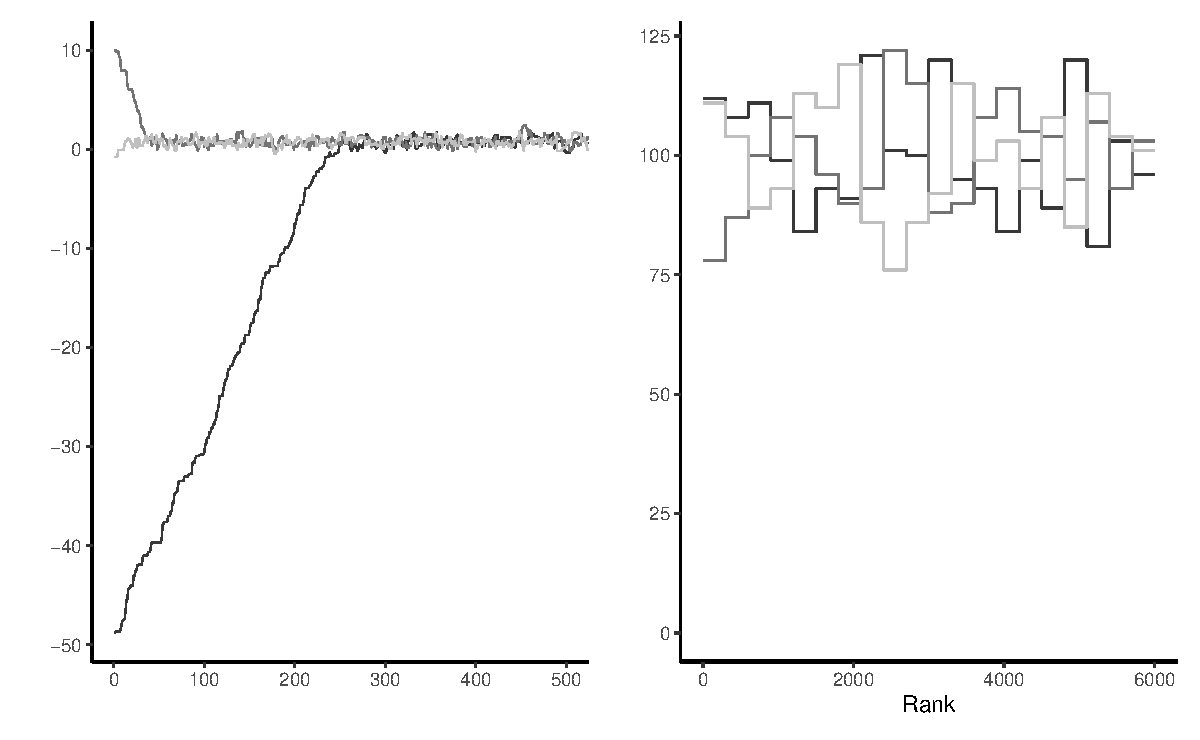
\includegraphics{mcmc_files/figure-pdf/fig-badstart-1.pdf}

}

\caption{\label{fig-badstart}Traceplots of three Markov chains for the
same target with different initial values for the first 500 iterations
(left) and trace rank plot after discarding these (right).}

\end{figure}

\hypertarget{diagnostics-of-convergence}{%
\subsection{Diagnostics of
convergence}\label{diagnostics-of-convergence}}

Generally, one would run a MCMC algorithm. The first iterations, used
during the burn in period to tune proposal variances and allow the
chains to converge to the stationary distribution, are discarded. If
visual inspection of the chains reveal that some of the chains for one
or more parameters are not stationary until some iteration, we will
discard all of these in addition.

The target of inference is functional (i.e., one-dimensional summaries
of the chain): we need to have convergence of the latter, but also
sufficient effective sample size for our averages to be accurate (at
least to two significant digits).

For the Poisson example, the effective sample size for the
\(\boldsymbol{\beta}\) for the multilevel model is a bit higher than
1000 with \(B=5000\) iterations, whereas we have for the simple naive
model is \ensuremath{10^{4}} for \(B=10000\) draws, suggesting
superefficient sampling. The dependency between \(\boldsymbol{\alpha}\)
and \(\boldsymbol{\beta}\) is responsible for the drop in accuracy.

The \texttt{coda} (convergence diagnosis and output analysis) \textbf{R}
package contains many tests. For example, the Geweke \(Z\)-score
compares the averages for the beginning and the end of the chain:
rejection of the null implies lack of convergence, or poor mixing.

Running multiple Markov chains can be useful for diagnostics. The
Gelman--Rubin diagnostic \(\widehat{R}\), also called potential scale
reduction statistic, is obtained by considering the difference between
within-chains and within-chains variance. Suppose we run \(M\) chains
for \(B\) iterations, post burn in. Denoting by \(\theta_{bm}\) the
\(b\)th draw of the \(m\)th chain, we compute the global average
\(\overline{\theta} = B^{-1}M^{-1}\sum_{b=1}^B \sum_{m=1}^m \theta_{bm}\)
and similarly the chain sample average and variances, respectively
\(\overline{\theta}_m\) and \(\widehat{\sigma}^2_m\)
(\(m=1, \ldots, M\)). The between-chain variance and within-chain
variance estimator are \begin{align*}
\mathsf{Va}_{\text{between}} &= \frac{B}{M-1}\sum_{m=1}^M (\overline{\theta}_m - \overline{\theta})^2\\
\mathsf{Va}_{\text{within}} &= \frac{1}{M}\sum_{m=1}^m \widehat{\sigma}^2_m
\end{align*} and we can compute \begin{align*}
\widehat{R} = \left(\frac{\mathsf{Va}_{\text{within}}(B-1) + \mathsf{Va}_{\text{between}}}{B\mathsf{Va}_{\text{within}}}\right)^{1/2}
\end{align*} The potential scale reduction statistic must be, by
construction, larger than 1 in large sample. Any value larger than this
is indicative of problems of convergence. While the Gelman--Rubin
diagnostic is frequently reported, and any value larger than 1 deemed
problematic, it is not enough to have approximately \(\widehat{R}=1\) to
guarantee convergence, but large values are usually indication of
something being amiss. Figure~\ref{fig-rhat} shows two instances where
the chains are visually very far from having the same average and this
is reflected by the large values of \(\widehat{R}\).

\begin{figure}[ht!]

{\centering 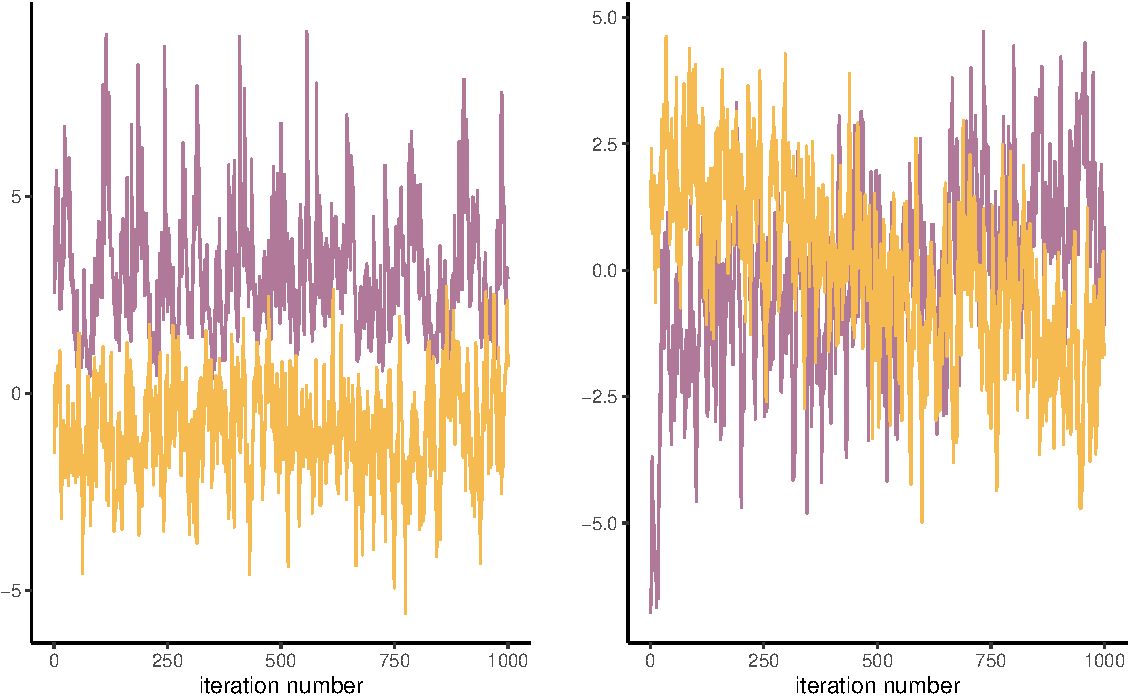
\includegraphics{mcmc_files/figure-pdf/fig-rhat-1.pdf}

}

\caption{\label{fig-rhat}Two pairs of Markov chains: the top ones seem
stationary, but with different modes. This makes the between chain
variance substantial, with a value of \(\widehat{R} \approx 3.4\),
whereas the chains on the right hover around the same values of zero,
but do not appear stable with \(\widehat{R} \approx 1.6\).}

\end{figure}

More generally, it is preferable to run a single chain for a longer
period than run multiple chains sequentially, as there is a cost to
initializing multiple times with different starting values since we must
discard initial draws. With parallel computations, multiple chains are
more frequent nowadays.

MCMC algorithms are often run thinning the chain (i.e., keeping only a
fraction of the samples drawn, typically every \(k\) iteration). This is
wasteful as we can of course get more precise estimates by keeping all
posterior draws, whether correlated or not. The only argument in favor
of thinning is limited storage capacity: if we run very long chains in a
model with hundreds of parameters, we may run out of memory.

\hypertarget{posterior-predictive-checks}{%
\subsection{Posterior predictive
checks}\label{posterior-predictive-checks}}

Posterior predictive checks can be used to compare models of varying
complexity: suppose we have the leave-one-out predictive distribution
for observation \(i\) given all the rest,
\(p(y_i \mid \boldsymbol{y}_{-i})\). We can assess the probability level
for each in turn, and the collection for all of leave-one-out cross
validation probabilities can be used to define the dis integral
transformation, consisting of being approximately uniform under the null
hypothesis of perfect model calibration. The probability of seeing an
outcome as extreme as \(y_i\) can be obtained by simulating draws from
the posterior predictive of \(\boldsymbol{y}_{-i}\) and computing the
scaled rank of the original observation. Values close to zero or one may
indicate outliers.

One of the visual diagnostics, outlined in Gabry et al.
(\protect\hyperlink{ref-Gabry:2019}{2019}), consists in computing a
summary statistic of interest from the posterior predictive (whether
mean, median, quantile, skewness, etc.) which is relevant for the
problem at hand and which we hope our model can adequately capture.

Suppose we have \(B\) draws from the posterior and simulate for each
\(n\) observations from the posterior predictive: we can benchmark
summary statistics from our original data \(\boldsymbol{y}\) with the
posterior predictive copies \(\widetilde{\boldsymbol{y}}_b\).
Figure~\ref{fig-posterior-pred-check} shows this for the two competing
models and highlight the fact that the simpler model is not dispersed
enough. Even the more complex model struggles to capture this additional
heterogeneity with the additional variables. One could go back to the
drawing board and consider a negative binomial model.

\begin{figure}[ht!]

{\centering 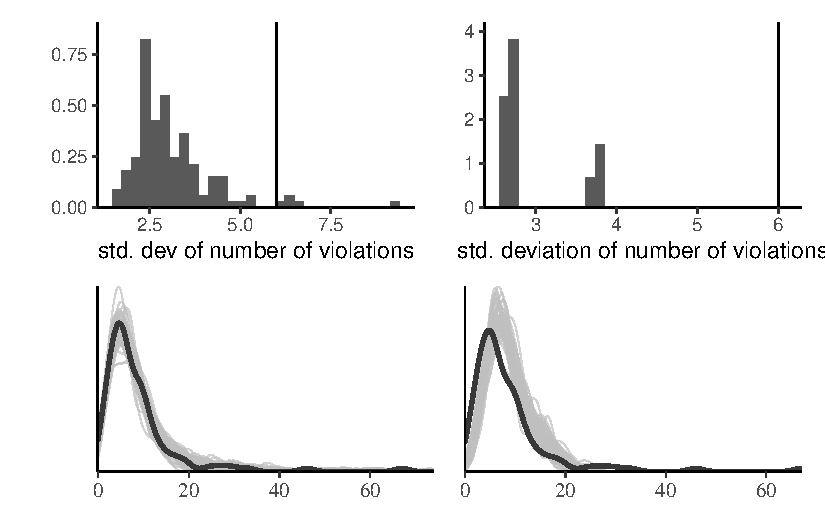
\includegraphics{mcmc_files/figure-pdf/fig-posterior-pred-check-1.pdf}

}

\caption{\label{fig-posterior-pred-check}Posterior predictive checks for
the standard deviation (top) and density of posterior draws (bottom) for
hierarchical Poisson model with individual effects (left) and simpler
model with only conditions (right).}

\end{figure}

\hypertarget{information-criterion}{%
\subsection{Information criterion}\label{information-criterion}}

The widely applicable information criterion
(\protect\hyperlink{ref-Watanabe:2010}{Watanabe 2010}) is a measure of
predictive performance that approximates the cross-validation loss.
Consider first the log pointwise predictive density, defined as the
expected value over the posterior distribution
\(p(\boldsymbol{\theta} \mid \boldsymbol{y})\), \begin{align*}
\mathsf{LPPD} = \mathsf{E}_{\boldsymbol{\theta} \mid \boldsymbol{y}} \left\{ \log p(y_i \mid \boldsymbol{\theta})\right\}.
\end{align*} We can approximate this quantity pointwise by averaging the
log density of each sample observation over the posterior samples via
Monte Carlo. The lower the value of \(\mathsf{LPPD}\), the better the
fit.

As in general information criteria, we add a penalization factor that
approximates the effective number of parameters in the model, with
\begin{align*}
n\mathsf{WAIC} = -\mathsf{LPPD} + \mathsf{Va}_{\boldsymbol{\theta} \mid \boldsymbol{y}}\{\log p(y_i \mid \boldsymbol{\theta})\}
\end{align*} where we use again the empirical variance to compute the
rightmost term. When comparing competing models, we can rely on their
values of \(\mathsf{WAIC}\) to discriminate about the predictive
performance. To compute \(\mathsf{WAIC}\), we need to store the values
of the log density of each observation, or at least minimally
\href{https://www.johndcook.com/blog/standard_deviation/}{compute the
running mean and variance accurately} pointwise at storage cost
\(\mathrm{O}(n)\). Note that Section 7.2 of Gelman et al.
(\protect\hyperlink{ref-Gelman:2013}{2013}) define the widely applicable
information criterion as \(2n \times \mathsf{WAIC}\) to make on par with
other information criteria, which are defined typically on the deviance
scale and so that lower values correspond to higher predictive
performance. For the smartwatch model, we get a value of 3.06 for the
complex model and 4.51: this suggests an improvement in using
individual-specific effects.

We can also compute the pointwise predictive performance using
leave-one-out validation. Naively, this requires refitting the model
\(n\) times, which is prohibitively expansive in the Bayesian setting
since this would require running the MCMC \(n\) times. A quick
approximation to the posterior predictive is via importance sampling,
but the latter can be noisy. The \texttt{loo} package uses this with
generalized Pareto smoothing to avoid overly large weights.

\begin{figure}[ht!]

{\centering 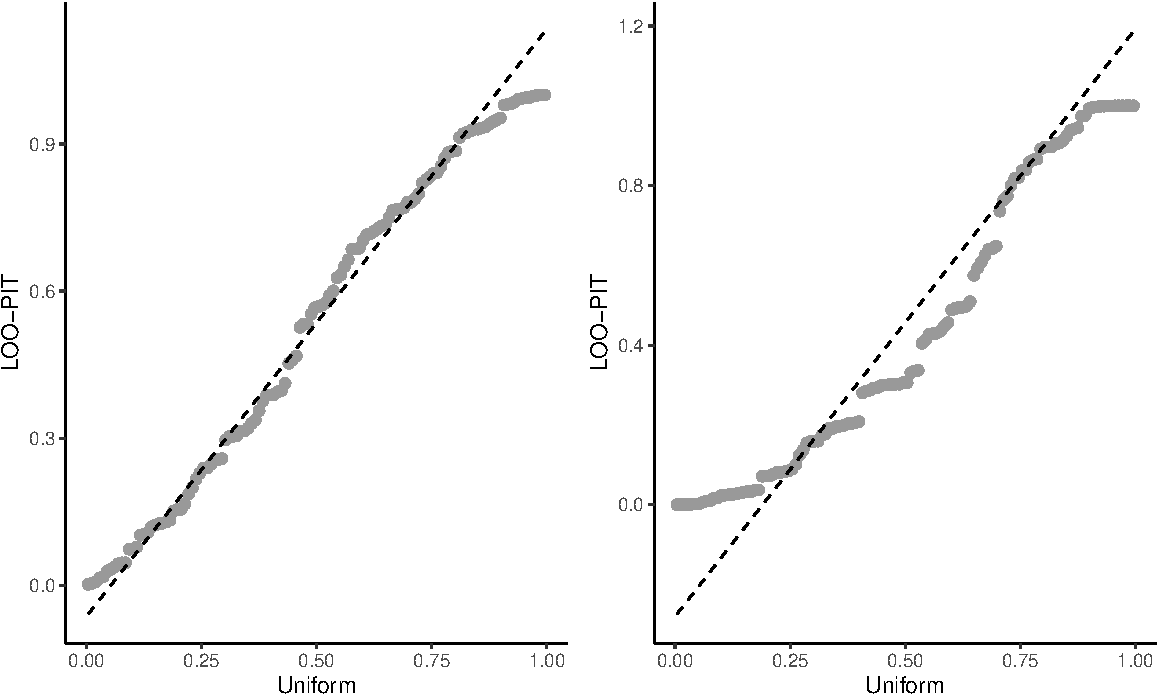
\includegraphics{mcmc_files/figure-pdf/fig-loocv-qqplots-1.pdf}

}

\caption{\label{fig-loocv-qqplots}Quantile-quantile plots based on
leave-one-out cross validation for model for the Poisson hierarchical
model with the individual random effects (left) and without (right).}

\end{figure}

\bookmarksetup{startatroot}

\hypertarget{references}{%
\chapter*{References}\label{references}}
\addcontentsline{toc}{chapter}{References}

\markboth{References}{References}

\hypertarget{refs}{}
\begin{CSLReferences}{1}{0}
\leavevmode\vadjust pre{\hypertarget{ref-Albert:2009}{}}%
Albert, Jim. 2009. \emph{Bayesian Computation with {R}}. 2nd ed. New
York: springer. \url{https://doi.org/10.1007/978-0-387-92298-0}.

\leavevmode\vadjust pre{\hypertarget{ref-Alexander:2023}{}}%
Alexander, Rohan. 2023. \emph{Telling Stories with Data: With
Applications in {R}}. Boca Raton, FL: CRC Press.

\leavevmode\vadjust pre{\hypertarget{ref-Andrieu.Thoms:2008}{}}%
Andrieu, Christophe, and Johannes Thoms. 2008. {``A Tutorial on Adaptive
{MCMC}.''} \emph{Statistics and Computing} 18 (4): 343--73.
\url{https://doi.org/10.1007/s11222-008-9110-y}.

\leavevmode\vadjust pre{\hypertarget{ref-LEcuyer.Botev:2017}{}}%
Botev, Zdravko, and Pierre L'Écuyer. 2017. {``Simulation from the Normal
Distribution Truncated to an Interval in the Tail.''} In
\emph{Proceedings of the 10th EAI International Conference on
Performance Evaluation Methodologies and Tools on 10th EAI International
Conference on Performance Evaluation Methodologies and Tools}, 23--29.
\url{https://doi.org/10.4108/eai.25-10-2016.2266879}.

\leavevmode\vadjust pre{\hypertarget{ref-Brodeur:2021}{}}%
Brodeur, Mathieu, Perrine Ruer, Pierre-Majorique Léger, and Sylvain
Sénécal. 2021. {``Smartwatches Are More Distracting Than Mobile Phones
While Driving: Results from an Experimental Study.''} \emph{Accident
Analysis \& Prevention} 149: 105846.
\url{https://doi.org/10.1016/j.aap.2020.105846}.

\leavevmode\vadjust pre{\hypertarget{ref-Coles.Tawn:1996}{}}%
Coles, Stuart G., and Jonathan A. Tawn. 1996. {``A {B}ayesian Analysis
of Extreme Rainfall Data.''} \emph{Journal of the Royal Statistical
Society. Series C (Applied Statistics)} 45 (4): 463--78.
\url{https://doi.org/10.2307/2986068}.

\leavevmode\vadjust pre{\hypertarget{ref-Devroye:1986}{}}%
Devroye, L. 1986. \emph{{Non-Uniform Random Variate Generation}}. New
York: Springer. \url{http://www.nrbook.com/devroye/}.

\leavevmode\vadjust pre{\hypertarget{ref-vanDyk.Meng:2001}{}}%
Dyk, David A van, and Xiao-Li Meng. 2001. {``The Art of Data
Augmentation.''} \emph{Journal of Computational and Graphical
Statistics} 10 (1): 1--50.
\url{https://doi.org/10.1198/10618600152418584}.

\leavevmode\vadjust pre{\hypertarget{ref-deFinetti:1974}{}}%
Finetti, Bruno de. 1974. \emph{Theory of Probability: A Critical
Introductory Treatment}. Vol. 1. New York: Wiley.

\leavevmode\vadjust pre{\hypertarget{ref-Gabry:2019}{}}%
Gabry, Jonah, Daniel Simpson, Aki Vehtari, Michael Betancourt, and
Andrew Gelman. 2019. {``{Visualization in {B}ayesian Workflow}.''}
\emph{Journal of the Royal Statistical Society Series A: Statistics in
Society} 182 (2): 389--402. \url{https://doi.org/10.1111/rssa.12378}.

\leavevmode\vadjust pre{\hypertarget{ref-Gelfand.Smith:1990}{}}%
Gelfand, Alan E., and Adrian F. M. Smith. 1990. {``Sampling-Based
Approaches to Calculating Marginal Densities.''} \emph{Journal of the
American Statistical Association} 85 (410): 398--409.
\url{https://doi.org/10.1080/01621459.1990.10476213}.

\leavevmode\vadjust pre{\hypertarget{ref-Gelman:2006}{}}%
Gelman, Andrew. 2006. {``Prior Distributions for Variance Parameters in
Hierarchical Models (Comment on Article by {B}rowne and {D}raper).''}
\emph{Bayesian Analysis} 1 (3): 515--34.
\url{https://doi.org/10.1214/06-BA117A}.

\leavevmode\vadjust pre{\hypertarget{ref-Gelman:2013}{}}%
Gelman, Andrew, John B. Carlin, Hal S. Stern, David B. Dunson, Aki
Vehtari, and Donald B. Rubin. 2013. \emph{Bayesian Data Analysis}. 3rd
ed. New York: Chapman; Hall/CRC. \url{https://doi.org/10.1201/b16018}.

\leavevmode\vadjust pre{\hypertarget{ref-Gelman:2020}{}}%
Gelman, Andrew, Aki Vehtari, Daniel Simpson, Charles C Margossian, Bob
Carpenter, Yuling Yao, Lauren Kennedy, Jonah Gabry, Paul-Christian
Bürkner, and Martin Modrák. 2020. {``Bayesian Workflow.''} \emph{arXiv}.
https://doi.org/\url{https://doi.org/10.48550/arXiv.2011.01808}.

\leavevmode\vadjust pre{\hypertarget{ref-Geman.Geman:1984}{}}%
Geman, Stuart, and Donald Geman. 1984. {``Stochastic Relaxation, {G}ibbs
Distributions, and the {B}ayesian Restoration of Images.''} \emph{IEEE
Transactions on Pattern Analysis and Machine Intelligence} PAMI-6 (6):
721--41. \url{https://doi.org/10.1109/TPAMI.1984.4767596}.

\leavevmode\vadjust pre{\hypertarget{ref-Geweke:2004}{}}%
Geweke, John. 2004. {``Getting It Right: Joint Distribution Tests of
Posterior Simulators.''} \emph{Journal of the American Statistical
Association} 99 (467): 799--804.
\url{https://doi.org/10.1198/016214504000001132}.

\leavevmode\vadjust pre{\hypertarget{ref-Geyer:2011}{}}%
Geyer, Charles J. 2011. {``Introduction to {M}arkov Chain {M}onte
{C}arlo.''} In \emph{Handbook of {M}arkov Chain {M}onte {C}arlo}, edited
by S. Brooks, A. Gelman, G. Jones, and X. L. Meng, 3--48. Boca Raton:
CRC Press. \url{https://doi.org/10.1201/b10905}.

\leavevmode\vadjust pre{\hypertarget{ref-Green:2001}{}}%
Green, Peter J. 2001. {``A Primer on {M}arkov Chain {M}onte {C}arlo.''}
\emph{Monographs on Statistics and Applied Probability} 87: 1--62.

\leavevmode\vadjust pre{\hypertarget{ref-Hastings:1970}{}}%
Hastings, W. K. 1970. {``{Monte {C}arlo sampling methods using {M}arkov
chains and their applications}.''} \emph{Biometrika} 57 (1): 97--109.
\url{https://doi.org/10.1093/biomet/57.1.97}.

\leavevmode\vadjust pre{\hypertarget{ref-Hobert:2011}{}}%
Hobert, James P. 2011. {``The Data Augmentation Algorithm: Theory and
Methodology.''} In \emph{Handbook of {M}arkov Chain {M}onte {C}arlo},
edited by S. Brooks, A. Gelman, G. Jones, and X. L. Meng, 253--94. Boca
Raton: CRC Press. \url{https://doi.org/10.1201/b10905}.

\leavevmode\vadjust pre{\hypertarget{ref-Kinderman.Monahan:1977}{}}%
Kinderman, Albert J, and John F Monahan. 1977. {``Computer Generation of
Random Variables Using the Ratio of Uniform Deviates.''} \emph{ACM
Transactions on Mathematical Software (TOMS)} 3 (3): 257--60.

\leavevmode\vadjust pre{\hypertarget{ref-Matias:2021}{}}%
Matias, J. Nathan, Kevin Munger, Marianne Aubin Le Quere, and Charles
Ebersole. 2021. {``The {U}pworthy {R}esearch {A}rchive, a Time Series of
32,487 Experiments in {U.S.} Media.''} \emph{Scientific Data} 8 (195).
\url{https://doi.org/10.1038/s41597-021-00934-7}.

\leavevmode\vadjust pre{\hypertarget{ref-McNeil.Frey.Embrechts:2005}{}}%
McNeil, A. J., R. Frey, and P. Embrechts. 2005. \emph{Quantitative Risk
Management: Concepts, Techniques, and Tools}. 1st ed. Princeton, NJ:
Princeton University Press.

\leavevmode\vadjust pre{\hypertarget{ref-Metropolis:1953}{}}%
Metropolis, Nicholas, Arianna W. Rosenbluth, Marshall N. Rosenbluth,
Augusta H. Teller, and Edward Teller. 1953. {``{Equation of State
Calculations by Fast Computing Machines}.''} \emph{The Journal of
Chemical Physics} 21 (6): 1087--92.
\url{https://doi.org/10.1063/1.1699114}.

\leavevmode\vadjust pre{\hypertarget{ref-Park.Casella:2008}{}}%
Park, Trevor, and George Casella. 2008. {``The {B}ayesian {L}asso.''}
\emph{Journal of the American Statistical Association} 103 (482):
681--86. \url{https://doi.org/10.1198/016214508000000337}.

\leavevmode\vadjust pre{\hypertarget{ref-Robert.Casella:2004}{}}%
Robert, Christian P., and George Casella. 2004. \emph{Monte {C}arlo
Statistical Methods}. New York, NY: Springer.
\url{https://doi.org/10.1007/978-1-4757-4145-2}.

\leavevmode\vadjust pre{\hypertarget{ref-Roberts.Rosenthal:2001}{}}%
Roberts, Gareth O., and Jeffrey S. Rosenthal. 2001. {``Optimal Scaling
for Various {M}etropolis--{H}astings Algorithms.''} \emph{Statistical
Science} 16 (4): 351--67. \url{https://doi.org/10.1214/ss/1015346320}.

\leavevmode\vadjust pre{\hypertarget{ref-Sherlock:2013}{}}%
Sherlock, Chris. 2013. {``Optimal Scaling of the Random Walk
{M}etropolis: General Criteria for the 0.234 Acceptance Rule.''}
\emph{Journal of Applied Probability} 50 (1): 1--15.
\url{https://doi.org/10.1239/jap/1363784420}.

\leavevmode\vadjust pre{\hypertarget{ref-Simpson:2017}{}}%
Simpson, Daniel, Håvard Rue, Andrea Riebler, Thiago G. Martins, and
Sigrunn H. Sørbye. 2017. {``Penalising Model Component Complexity: A
Principled, Practical Approach to Constructing Priors.''}
\emph{Statistical Science} 32 (1): 1--28.
\url{https://doi.org/10.1214/16-STS576}.

\leavevmode\vadjust pre{\hypertarget{ref-Sorbye.Rue:2017}{}}%
Sørbye, Sigrunn Holbek, and Håvard Rue. 2017. {``Penalised Complexity
Priors for Stationary Autoregressive Processes.''} \emph{Journal of Time
Series Analysis} 38 (6): 923--35.
\url{https://doi.org/10.1111/jtsa.12242}.

\leavevmode\vadjust pre{\hypertarget{ref-Tanner.Wong:1987}{}}%
Tanner, Martin A., and Wing Hung Wong. 1987. {``The Calculation of
Posterior Distributions by Data Augmentation.''} \emph{Journal of the
American Statistical Association} 82 (398): 528--40.
\url{https://doi.org/10.1080/01621459.1987.10478458}.

\leavevmode\vadjust pre{\hypertarget{ref-Wakefield:1991}{}}%
Wakefield, J. C., A. E. Gelfand, and A. F. M. Smith. 1991. {``Efficient
Generation of Random Variates via the Ratio-of-Uniforms Method.''}
\emph{Statistics and Computing} 1 (2): 129--33.
\url{https://doi.org/10.1007/BF01889987}.

\leavevmode\vadjust pre{\hypertarget{ref-Watanabe:2010}{}}%
Watanabe, Sumio. 2010. {``Asymptotic Equivalence of {B}ayes Cross
Validation and Widely Applicable Information Criterion in Singular
Learning Theory.''} \emph{Journal of Machine Learning Research} 11
(116): 3571--94. \url{http://jmlr.org/papers/v11/watanabe10a.html}.

\end{CSLReferences}


\backmatter

\end{document}
